\documentclass[pra,superscriptaddress,reprint,amsmath,amssymb,nofootinbib]{revtex4-2}
%DIF LATEXDIFF DIFFERENCE FILE
%DIF DEL old.tex   Thu Oct  5 15:27:52 2023
%DIF ADD new.tex   Thu Oct  5 15:22:13 2023

\usepackage{graphicx}
\usepackage{dcolumn}
\usepackage{subfiles} 
\usepackage{bm}
%for nice coloured hyperlinks:
\usepackage[usenames,dvipsnames]{xcolor}
\usepackage[pdftex,plainpages=false,colorlinks=true]{hyperref}
\usepackage[toc,page,title,titletoc,header]{appendix} 
\usepackage{multirow}
\usepackage{tabularx}
%\usepackage[bottom]{footmisc}
%\usepackage{caption}
%\usepackage{subcaption}
%\usepackage[bottom]{footmisc}
%\usepackage{soul}
\usepackage{algorithm}
\usepackage{algpseudocode}
\algnewcommand{\To}{\textbf{To }}
\algnewcommand\Input{\item[\textbf{Initialisation:}]}%
\algnewcommand\Output{\item[\textbf{Output:}]}%
\usepackage{booktabs}

%%%%%%%%%%%%%%%%%%%%%%%%%%%%%%%%%%%%%%%%%%%%%%%%%%

%%%%% AUTHORS - PLACE YOUR OWN COMMANDS HERE %%%%%

% notes
\newcommand{\han}{\textcolor{orange}}
\usepackage[caption=false]{subfig}

%DIF 33a33-34
\usepackage[normalem]{ulem} %DIF > 
 %DIF > 
%DIF -------
%\usepackage[section]{placeins} %ensures figures go in their section e.g https://tex.stackexchange.com/questions/279/how-do-i-ensure-that-figures-appear-in-the-section-theyre-associated-with


% units
\newcommand{\Hz}{\mathrm{Hz}}
\newcommand{\ms}{\mathrm{ms}}
\newcommand{\secs}{\mathrm{s}}


% variables
\newcommand{\omegahigh}{\omega_{\mathrm{high}}}
\newcommand{\omegalow}{\omega_{\mathrm{low}}}
\newcommand{\fgw}{f_{\mathrm{gw}}}
\newcommand{\fline}{f_{\mathrm{line}}}

\newcommand{\CSOneName}{\texttt{H1:PEM-CS\_MAINSMON\_EBAY\_1\_DQ}}

\newcommand{\StrainChanName}{\texttt{L1:DCS-CALIB\_STRAIN\_C01\_AR}}
\newcommand{\PEMChanName}{\texttt{L1:PEM-CS\_MAINSMON\_EBAY\_1\_DQ}}
%%%%%%%%%%%%%%%%%%%%%%%%%%%%%%%%%%%%%%%%%%%%%%%%%%




%\let\oldfootnote\footnote
%\renewcommand{\footnote}[1]{%
%	\begingroup%
%	\linespread{1}%    % <- linespread for footnote: 1, 1.1, 1.2 etc
%	\oldfootnote{#1}%
%	\endgroup%
%}
%
%\interfootnotelinepenalty=10000






%%%%%%%%%%%%%%%%%%% TITLE PAGE %%%%%%%%%%%%%%%%%%%
%DIF PREAMBLE EXTENSION ADDED BY LATEXDIFF
%DIF UNDERLINE PREAMBLE %DIF PREAMBLE
\RequirePackage[normalem]{ulem} %DIF PREAMBLE
\RequirePackage{color}\definecolor{RED}{rgb}{1,0,0}\definecolor{BLUE}{rgb}{0,0,1} %DIF PREAMBLE
\providecommand{\DIFaddtex}[1]{{\protect\color{blue}\uwave{#1}}} %DIF PREAMBLE
\providecommand{\DIFdeltex}[1]{{\protect\color{red}\sout{#1}}}                      %DIF PREAMBLE
%DIF SAFE PREAMBLE %DIF PREAMBLE
\providecommand{\DIFaddbegin}{} %DIF PREAMBLE
\providecommand{\DIFaddend}{} %DIF PREAMBLE
\providecommand{\DIFdelbegin}{} %DIF PREAMBLE
\providecommand{\DIFdelend}{} %DIF PREAMBLE
\providecommand{\DIFmodbegin}{} %DIF PREAMBLE
\providecommand{\DIFmodend}{} %DIF PREAMBLE
%DIF FLOATSAFE PREAMBLE %DIF PREAMBLE
\providecommand{\DIFaddFL}[1]{\DIFadd{#1}} %DIF PREAMBLE
\providecommand{\DIFdelFL}[1]{\DIFdel{#1}} %DIF PREAMBLE
\providecommand{\DIFaddbeginFL}{} %DIF PREAMBLE
\providecommand{\DIFaddendFL}{} %DIF PREAMBLE
\providecommand{\DIFdelbeginFL}{} %DIF PREAMBLE
\providecommand{\DIFdelendFL}{} %DIF PREAMBLE
%DIF HYPERREF PREAMBLE %DIF PREAMBLE
\providecommand{\DIFadd}[1]{\texorpdfstring{\DIFaddtex{#1}}{#1}} %DIF PREAMBLE
\providecommand{\DIFdel}[1]{\texorpdfstring{\DIFdeltex{#1}}{}} %DIF PREAMBLE
\newcommand{\DIFscaledelfig}{0.5}
%DIF HIGHLIGHTGRAPHICS PREAMBLE %DIF PREAMBLE
\RequirePackage{settobox} %DIF PREAMBLE
\RequirePackage{letltxmacro} %DIF PREAMBLE
\newsavebox{\DIFdelgraphicsbox} %DIF PREAMBLE
\newlength{\DIFdelgraphicswidth} %DIF PREAMBLE
\newlength{\DIFdelgraphicsheight} %DIF PREAMBLE
% store original definition of \includegraphics %DIF PREAMBLE
\LetLtxMacro{\DIFOincludegraphics}{\includegraphics} %DIF PREAMBLE
\newcommand{\DIFaddincludegraphics}[2][]{{\color{blue}\fbox{\DIFOincludegraphics[#1]{#2}}}} %DIF PREAMBLE
\newcommand{\DIFdelincludegraphics}[2][]{% %DIF PREAMBLE
\sbox{\DIFdelgraphicsbox}{\DIFOincludegraphics[#1]{#2}}% %DIF PREAMBLE
\settoboxwidth{\DIFdelgraphicswidth}{\DIFdelgraphicsbox} %DIF PREAMBLE
\settoboxtotalheight{\DIFdelgraphicsheight}{\DIFdelgraphicsbox} %DIF PREAMBLE
\scalebox{\DIFscaledelfig}{% %DIF PREAMBLE
\parbox[b]{\DIFdelgraphicswidth}{\usebox{\DIFdelgraphicsbox}\\[-\baselineskip] \rule{\DIFdelgraphicswidth}{0em}}\llap{\resizebox{\DIFdelgraphicswidth}{\DIFdelgraphicsheight}{% %DIF PREAMBLE
\setlength{\unitlength}{\DIFdelgraphicswidth}% %DIF PREAMBLE
\begin{picture}(1,1)% %DIF PREAMBLE
\thicklines\linethickness{2pt} %DIF PREAMBLE
{\color[rgb]{1,0,0}\put(0,0){\framebox(1,1){}}}% %DIF PREAMBLE
{\color[rgb]{1,0,0}\put(0,0){\line( 1,1){1}}}% %DIF PREAMBLE
{\color[rgb]{1,0,0}\put(0,1){\line(1,-1){1}}}% %DIF PREAMBLE
\end{picture}% %DIF PREAMBLE
}\hspace*{3pt}}} %DIF PREAMBLE
} %DIF PREAMBLE
\LetLtxMacro{\DIFOaddbegin}{\DIFaddbegin} %DIF PREAMBLE
\LetLtxMacro{\DIFOaddend}{\DIFaddend} %DIF PREAMBLE
\LetLtxMacro{\DIFOdelbegin}{\DIFdelbegin} %DIF PREAMBLE
\LetLtxMacro{\DIFOdelend}{\DIFdelend} %DIF PREAMBLE
\DeclareRobustCommand{\DIFaddbegin}{\DIFOaddbegin \let\includegraphics\DIFaddincludegraphics} %DIF PREAMBLE
\DeclareRobustCommand{\DIFaddend}{\DIFOaddend \let\includegraphics\DIFOincludegraphics} %DIF PREAMBLE
\DeclareRobustCommand{\DIFdelbegin}{\DIFOdelbegin \let\includegraphics\DIFdelincludegraphics} %DIF PREAMBLE
\DeclareRobustCommand{\DIFdelend}{\DIFOaddend \let\includegraphics\DIFOincludegraphics} %DIF PREAMBLE
\LetLtxMacro{\DIFOaddbeginFL}{\DIFaddbeginFL} %DIF PREAMBLE
\LetLtxMacro{\DIFOaddendFL}{\DIFaddendFL} %DIF PREAMBLE
\LetLtxMacro{\DIFOdelbeginFL}{\DIFdelbeginFL} %DIF PREAMBLE
\LetLtxMacro{\DIFOdelendFL}{\DIFdelendFL} %DIF PREAMBLE
\DeclareRobustCommand{\DIFaddbeginFL}{\DIFOaddbeginFL \let\includegraphics\DIFaddincludegraphics} %DIF PREAMBLE
\DeclareRobustCommand{\DIFaddendFL}{\DIFOaddendFL \let\includegraphics\DIFOincludegraphics} %DIF PREAMBLE
\DeclareRobustCommand{\DIFdelbeginFL}{\DIFOdelbeginFL \let\includegraphics\DIFdelincludegraphics} %DIF PREAMBLE
\DeclareRobustCommand{\DIFdelendFL}{\DIFOaddendFL \let\includegraphics\DIFOincludegraphics} %DIF PREAMBLE
%DIF COLORLISTINGS PREAMBLE %DIF PREAMBLE
\RequirePackage{listings} %DIF PREAMBLE
\RequirePackage{color} %DIF PREAMBLE
\lstdefinelanguage{DIFcode}{ %DIF PREAMBLE
%DIF DIFCODE_UNDERLINE %DIF PREAMBLE
  moredelim=[il][\color{red}\sout]{\%DIF\ <\ }, %DIF PREAMBLE
  moredelim=[il][\color{blue}\uwave]{\%DIF\ >\ } %DIF PREAMBLE
} %DIF PREAMBLE
\lstdefinestyle{DIFverbatimstyle}{ %DIF PREAMBLE
	language=DIFcode, %DIF PREAMBLE
	basicstyle=\ttfamily, %DIF PREAMBLE
	columns=fullflexible, %DIF PREAMBLE
	keepspaces=true %DIF PREAMBLE
} %DIF PREAMBLE
\lstnewenvironment{DIFverbatim}{\lstset{style=DIFverbatimstyle}}{} %DIF PREAMBLE
\lstnewenvironment{DIFverbatim*}{\lstset{style=DIFverbatimstyle,showspaces=true}}{} %DIF PREAMBLE
%DIF END PREAMBLE EXTENSION ADDED BY LATEXDIFF

\begin{document}
\preprint{}

\title[test short title]{Adaptive cancellation of \DIFaddbegin \DIFadd{mains }\DIFaddend power \DIFdelbegin \DIFdel{grid }\DIFdelend interference in continuous gravitational wave searches with a hidden \DIFdelbegin \DIFdel{markov }\DIFdelend \DIFaddbegin \DIFadd{Markov }\DIFaddend model}% Force line breaks with \\
%\thanks{this would be a footnoted on the first page}%

%\input{authors.tex}

\author{Author 1, Author 2, etc. Kimpson, \DIFdelbegin \DIFdel{Suvrova}\DIFdelend \DIFaddbegin \DIFadd{Suvorova}\DIFaddend , Liu, Melatos, Middleton, Evans, Moran, Meyers, any others?}
\date{\today}% It is always \today, today,
             %  but any date may be explicitly specified


\begin{abstract}
		Continuous gravitational wave \DIFdelbegin \DIFdel{(GW) searches are commonly }\DIFdelend \DIFaddbegin \DIFadd{searches with terrestrial, long-baseline interferometers are }\DIFaddend hampered by long-lived, \DIFdelbegin \DIFdel{narrow peaks in the instrumental frequency spectra known as `lines'}\DIFdelend \DIFaddbegin \DIFadd{narrowband features in the power spectral density of the detector noise, known as lines}\DIFaddend . Candidate GW signals which \DIFdelbegin \DIFdel{lie within frequency bands }\DIFdelend \DIFaddbegin \DIFadd{overlap spectrally }\DIFaddend with known lines are typically vetoed. \DIFdelbegin \DIFdel{In this work }\DIFdelend \DIFaddbegin \DIFadd{Here }\DIFaddend we demonstrate a \DIFdelbegin \DIFdel{new }\DIFdelend line subtraction method based on adaptive noise cancellation\DIFdelbegin \DIFdel{(ANC). ANC is common }\DIFdelend \DIFaddbegin \DIFadd{, using a recursive least squares algorithm, a common approach }\DIFaddend in electrical engineering applications, \DIFdelbegin \DIFdel{including for }\DIFdelend \DIFaddbegin \DIFadd{such as }\DIFaddend processing audio and biomedical signals. We \DIFdelbegin \DIFdel{show how ANC can be used in conjunction with a Viterbi search to track spin-wandering continuous wave signals near the LIGO }\DIFdelend \DIFaddbegin \DIFadd{validate the line subtraction method by combining it with a hidden Markov model, a standard continuous wave search tool, to detect a synthetic continuous wave signal with an unknown and randomly wandering frequency which overlaps with the strong mains power line at $60 \, {\rm Hz}$ in the Laser Interferometer Gravitational Wave Observatory. We show that the synthetic continuous wave signal can be successfully recovered once the }\DIFaddend 60 Hz line \DIFdelbegin \DIFdel{. 
}\DIFdelend \DIFaddbegin \DIFadd{has been subtracted. The performance of the line subtraction method with respect to the characteristics of the 60 Hz line and the parameters of the method is explored and quantified.
		}

\DIFaddend \begin{description}
\item[DOI]
\end{description}
\end{abstract}



\maketitle	


\section{Introduction} \label{sec:intro}
Instrumental noise artifacts in gravitational wave (GW) searches with terrestrial, long-baseline interferometers are classified according to their duration and spectral properties.  Short-lived, non-stationary\DIFaddbegin \DIFadd{, }\DIFaddend recurrent noise events such as optomechanical glitches typically last for seconds and exhibit distinctive spectral signatures, e.g they can be chirp-like \cite{Blackburn2008,Aasi2012,Aasi2015,DetCharGW150914:2016,Glanzer2023}. Long-lived, quasi-stationary, broadband noise sources include seismic disturbances at low frequencies, test mass thermal fluctuations at intermediate frequencies, and photon shot noise at high frequencies \cite{AasiEtAlAdLIGO:2015,LIGOnoiseguide,VIROGnoise,Akutsu2021PTEP,Nguyen2021}. Long-lived narrowband spectral artifacts \DIFdelbegin \DIFdel{- }\DIFdelend \DIFaddbegin \DIFadd{--- }\DIFaddend termed instrumental lines \DIFdelbegin \DIFdel{- }\DIFdelend \DIFaddbegin \DIFadd{--- }\DIFaddend are caused by electrical subsystems (e.g. mains power, clocks, oscillators), mechanical subsystems (e.g. test mass and beam-splitter violin modes) and calibration processes \cite{CovasEtAl:2018}, although \DIFdelbegin \DIFdel{often }\DIFdelend \DIFaddbegin \DIFadd{sometimes }\DIFaddend the origin of a specific feature is unknown. Instrumental lines are disruptive, especially for continuous wave (CW) searches where the target astrophysical signal is quasi-monochromatic and resembles the noise artifact spectrally. Many above-threshold candidates discovered in \DIFdelbegin \DIFdel{CW searches to date }\DIFdelend \DIFaddbegin \DIFadd{published CW searches }\DIFaddend are vetoed because they coincide with known instrumental lines \cite{Piccinni2022,Riles2023,Wette2023}, for instance, in \DIFdelbegin \DIFdel{CW searches involving }\DIFdelend data from Observing Run 3 (O3) with the Laser Interferometer Gravitational Wave Observatory (LIGO), Virgo and the Kamioka Gravitational Wave Detector (KAGRA)  \cite[e.g.][]{Ligo_lineveto1,ligo_lineveto2,ligo_lineveto3} \newline 


Several techniques have been implemented by the LIGO-Virgo-KAGRA (LVK) \DIFdelbegin \DIFdel{collaboration }\DIFdelend \DIFaddbegin \DIFadd{Collaboration }\DIFaddend to identify, characterize and suppress instrumental noise artifacts \cite{Davis2021,Davisgalaxies10010012}. Some techniques identify and veto an artifact (or gate \DIFdelbegin \DIFdel{a segments of the data }\DIFdelend \DIFaddbegin \DIFadd{data segments}\DIFaddend ) based on its time-frequency signature \cite{Abbott2018CQVeto,Lee2021,Steltner2022Ph}. Other techniques perform offline noise subtraction with reference to auxiliary data from physical environmental monitors (PEMs) \cite{Driggers2012RScI,Tiwari2015,Davis2019,Driggers2019}. PEMs can be used to witness correlated noise and generate a reference signal directly or elucidate and quantify multichannel couplings \cite{Jung2022PRD,marin1997}. \DIFdelbegin \DIFdel{Finally }\DIFdelend \DIFaddbegin \DIFadd{Additionally }\DIFaddend some techniques are based on machine learning \cite{Cuoco2020,Vajente2020PhR,OrmistonEtAl:2020,Yamamoto2023}. In CW searches specifically, the distinctive amplitude and frequency (Doppler) modulations associated with the \DIFdelbegin \DIFdel{Earths }\DIFdelend \DIFaddbegin \DIFadd{Earth's }\DIFaddend rotation and revolution \DIFaddbegin \DIFadd{respectively }\DIFaddend can be exploited to discriminate between terrestrial noise artifacts and astrophysical signals \cite{Zhu2017PhRvD,JonesPhysRevD.106.123011}.  \newline 

In most  of the situations above, the practical effect of an instrumental line is to excise the relevant part of the observing band from a CW search. That is, if an above threshold CW search candidate coincides with a known instrumental line, the candidate is vetoed under current practice without further analysis, such as comparing the expected strength of the noise line with the measured strength of the candidate \footnote{A regularly updated log of narrowband instrumental lines in the LVK detector is maintained at \href{https://dcc.ligo.org/LIGO-T2100200/public}{dcc.ligo.org/LIGO-T2100200/public} for public reference\DIFaddbegin \DIFadd{.}\DIFaddend }. In this paper we take a first step towards lifting the above limitation. We introduce an adaptive noise cancellation (ANC) scheme  based on an adaptive recursive least squares (ARLS) method which suppresses narrowband noise proportional to a known PEM reference signal. We then apply the ANC scheme to a CW search algorithm based on a hidden Markov model (HMM) which detects and tracks quasi-monochromatic GW signals with wandering frequency and has been tested and validated thoroughly in multiple LVK searches \cite{Suvorova2016PhRv,Piccinni2022,Riles2023,Wette2023}. We demonstrate with synthetic data that the ANC scheme and HMM algorithm together can successfully detect a GW signal lying under the \DIFdelbegin \DIFdel{60Hz }\DIFdelend \DIFaddbegin \DIFadd{60 Hz }\DIFaddend mains power line, if the signal exceeds a well-defined minimum amplitude. The approach extends naturally to other instrumental lines, a topic for future work. \newline 

The paper is organized as follows. In Section \ref{sec:pgi} we outline \DIFdelbegin \DIFdel{our }\DIFdelend \DIFaddbegin \DIFadd{a }\DIFaddend mathematical model for the \DIFdelbegin \DIFdel{60Hz mains power spectral }\DIFdelend \DIFaddbegin \DIFadd{60 Hz mains power }\DIFaddend line and the PEM reference signal, and justify the assumptions of the model by reference to \DIFdelbegin \DIFdel{the strain and environmental }\DIFdelend data from the LIGO Livingston interferometer.  In Section \ref{sec:method} we introduce ANC formulated as an ARLS method. \DIFdelbegin \DIFdel{We go on in Section \ref{sec:results} to deploy the ANC method }\DIFdelend \DIFaddbegin \DIFadd{In Section \ref{sec:results} we validate the ANC scheme on synthetic GW strain data, }\DIFaddend in conjunction with an HMM Viterbi \DIFdelbegin \DIFdel{solver applied to synthetic GW strain data }\DIFdelend \DIFaddbegin \DIFadd{algorithm, }\DIFaddend and demonstrate the successful recovery of a \DIFdelbegin \DIFdel{monochromatic GW signal. }\DIFdelend \DIFaddbegin \DIFadd{frequency-wandering CW signal. In Section \ref{sec:theroccurves} we quantify the performance of the HMM Viterbi algorithm and ANC scheme as a function of the key parameters of the mains power interference and ANC filter. Concluding remarks are given in Section \ref{sec:conclusions}.
}\DIFaddend 

\section{Power grid interference} \label{sec:pgi}
The goal of this paper is to detect a \DIFdelbegin \DIFdel{quasi-normal }\DIFdelend \DIFaddbegin \DIFadd{quasi-monochromatic }\DIFaddend GW signal in a data stream contaminated by two kinds of noise: additive Gaussian noise which is fundamental and irreducible, and additive non-Gaussian interference from a long-lived narrow spectral feature which can be filtered out in principle given an accurately measured reference signal. For this work we consider the spectral line at 60 Hz that results from the North American alternating current power grid as the additive non-Gaussian interference\DIFaddbegin \DIFadd{, as it is a long-standing impediment to many CW searches with the LIGO interferometers}\DIFaddend . In Section \ref{sec22} we briefly review the 60 Hz LIGO interference line before proceeding in Section \ref{sec21} to specify the assumed mathematical forms of the interference and reference signals. In Section \ref{sec23} we justify the assumptions of Section \ref{sec21} by analysing differential arm length (DARM channel) and environmental (power grid monitoring) data from the LIGO interferometers. 


\subsection{LIGO 60 Hz Interference}  \label{sec22}
%Useful literature: https://journals.aps.org/prd/pdf/10.1103/PhysRevD.97.082002

LIGO data contains multiple long-duration narrow lines \DIFdelbegin \DIFdel{(e.g. Fig. \ref{fig:strainSensitivity}) }\DIFdelend in addition to the usual Gaussian noise. \DIFdelbegin \DIFdel{The }\DIFdelend \DIFaddbegin \DIFadd{These lines are shown in Figure \ref{fig:strainSensitivity} where we plot the amplitude spectral density of the GW strain channel }\texttt{\DIFadd{*:DCS-CALIB\_STRAIN\_C01\_AR}} \DIFadd{for both LIGO-Hanford (}\texttt{\DIFadd{H1}}\DIFadd{, orange curve) and LIGO-Livingston (}\texttt{\DIFadd{L1}}\DIFadd{, blue curve). The small amplitude random fluctuations are the result of Gaussian noise whereas the large amplitude spikes are the long-duration lines. The }\DIFaddend provision of mains power electricity in North America via an alternating current with frequency 60 Hz leads to a line in the \DIFdelbegin \DIFdel{LIGO data at the corresponding frequency. The coupling between the mains power and the gravitational wave data channelcan occur since }\DIFdelend \DIFaddbegin \DIFadd{power spectral density of the LIGO noise. The mains power couples to the GW strain channel, because }\DIFaddend the performance of the high-sensitivity electronic components within LIGO varies with respect to the input power voltage. Additionally, the magnetic fields that arise from the AC mains supply \DIFdelbegin \DIFdel{can couple with the magnets on the LIGO }\DIFdelend \DIFaddbegin \DIFadd{couple to magnets on }\DIFaddend optical components. \DIFdelbegin \DIFdel{Whilst some }\DIFdelend \DIFaddbegin \newline 

\DIFadd{Some }\DIFaddend spectral lines are static, \DIFdelbegin \DIFdel{the 60Hz }\DIFdelend \DIFaddbegin \DIFadd{but the 60 Hz }\DIFaddend line wanders in time, due to variations in the load in the North \DIFdelbegin \DIFdel{America power gridat any one time (e.g. Fig. \ref{fig:powerCascade}). This time variation can further impact the detector sensitivity over a broader frequency band. }\DIFdelend \DIFaddbegin \DIFadd{American power grid. The wandering is displayed in the cascade plot in Figure \ref{fig:powerCascade}, where the amplitude spectral density of the output signal of the LIGO-Hanford PEM channel }\CSOneName \DIFadd{\, is plotted for 210 5-min samples stacked vertically. The peak of the amplitude spectral density varies from 59.969 Hz  to 60.053 Hz, across the 210 samples with an average value of 60.004 Hz. Its full width half maximum varies from 5.294 mHz to 29.377 mHz, with an average value of 10.749  mHz. }\DIFaddend For a full review of LIGO spectral artifacts, including the 60 Hz line, we refer the reader to \cite{CovasEtAl:2018}. \DIFaddbegin \newline 


\DIFadd{The $60 \, {\rm Hz}$ line occurs in the neighbourhood of plausible astrophysical signals. For example, mass quadrupole radiation from a rotating mountain on the Crab pulsar would be emitted at twice the star's spin frequency, viz. $30.2 \, {\rm Hz}$ \mbox{%DIFAUXCMD
\citep{Riles2023,Wette2023}}\hskip0pt%DIFAUXCMD
.
}


\DIFaddend \begin{figure}
	\begin{center}
		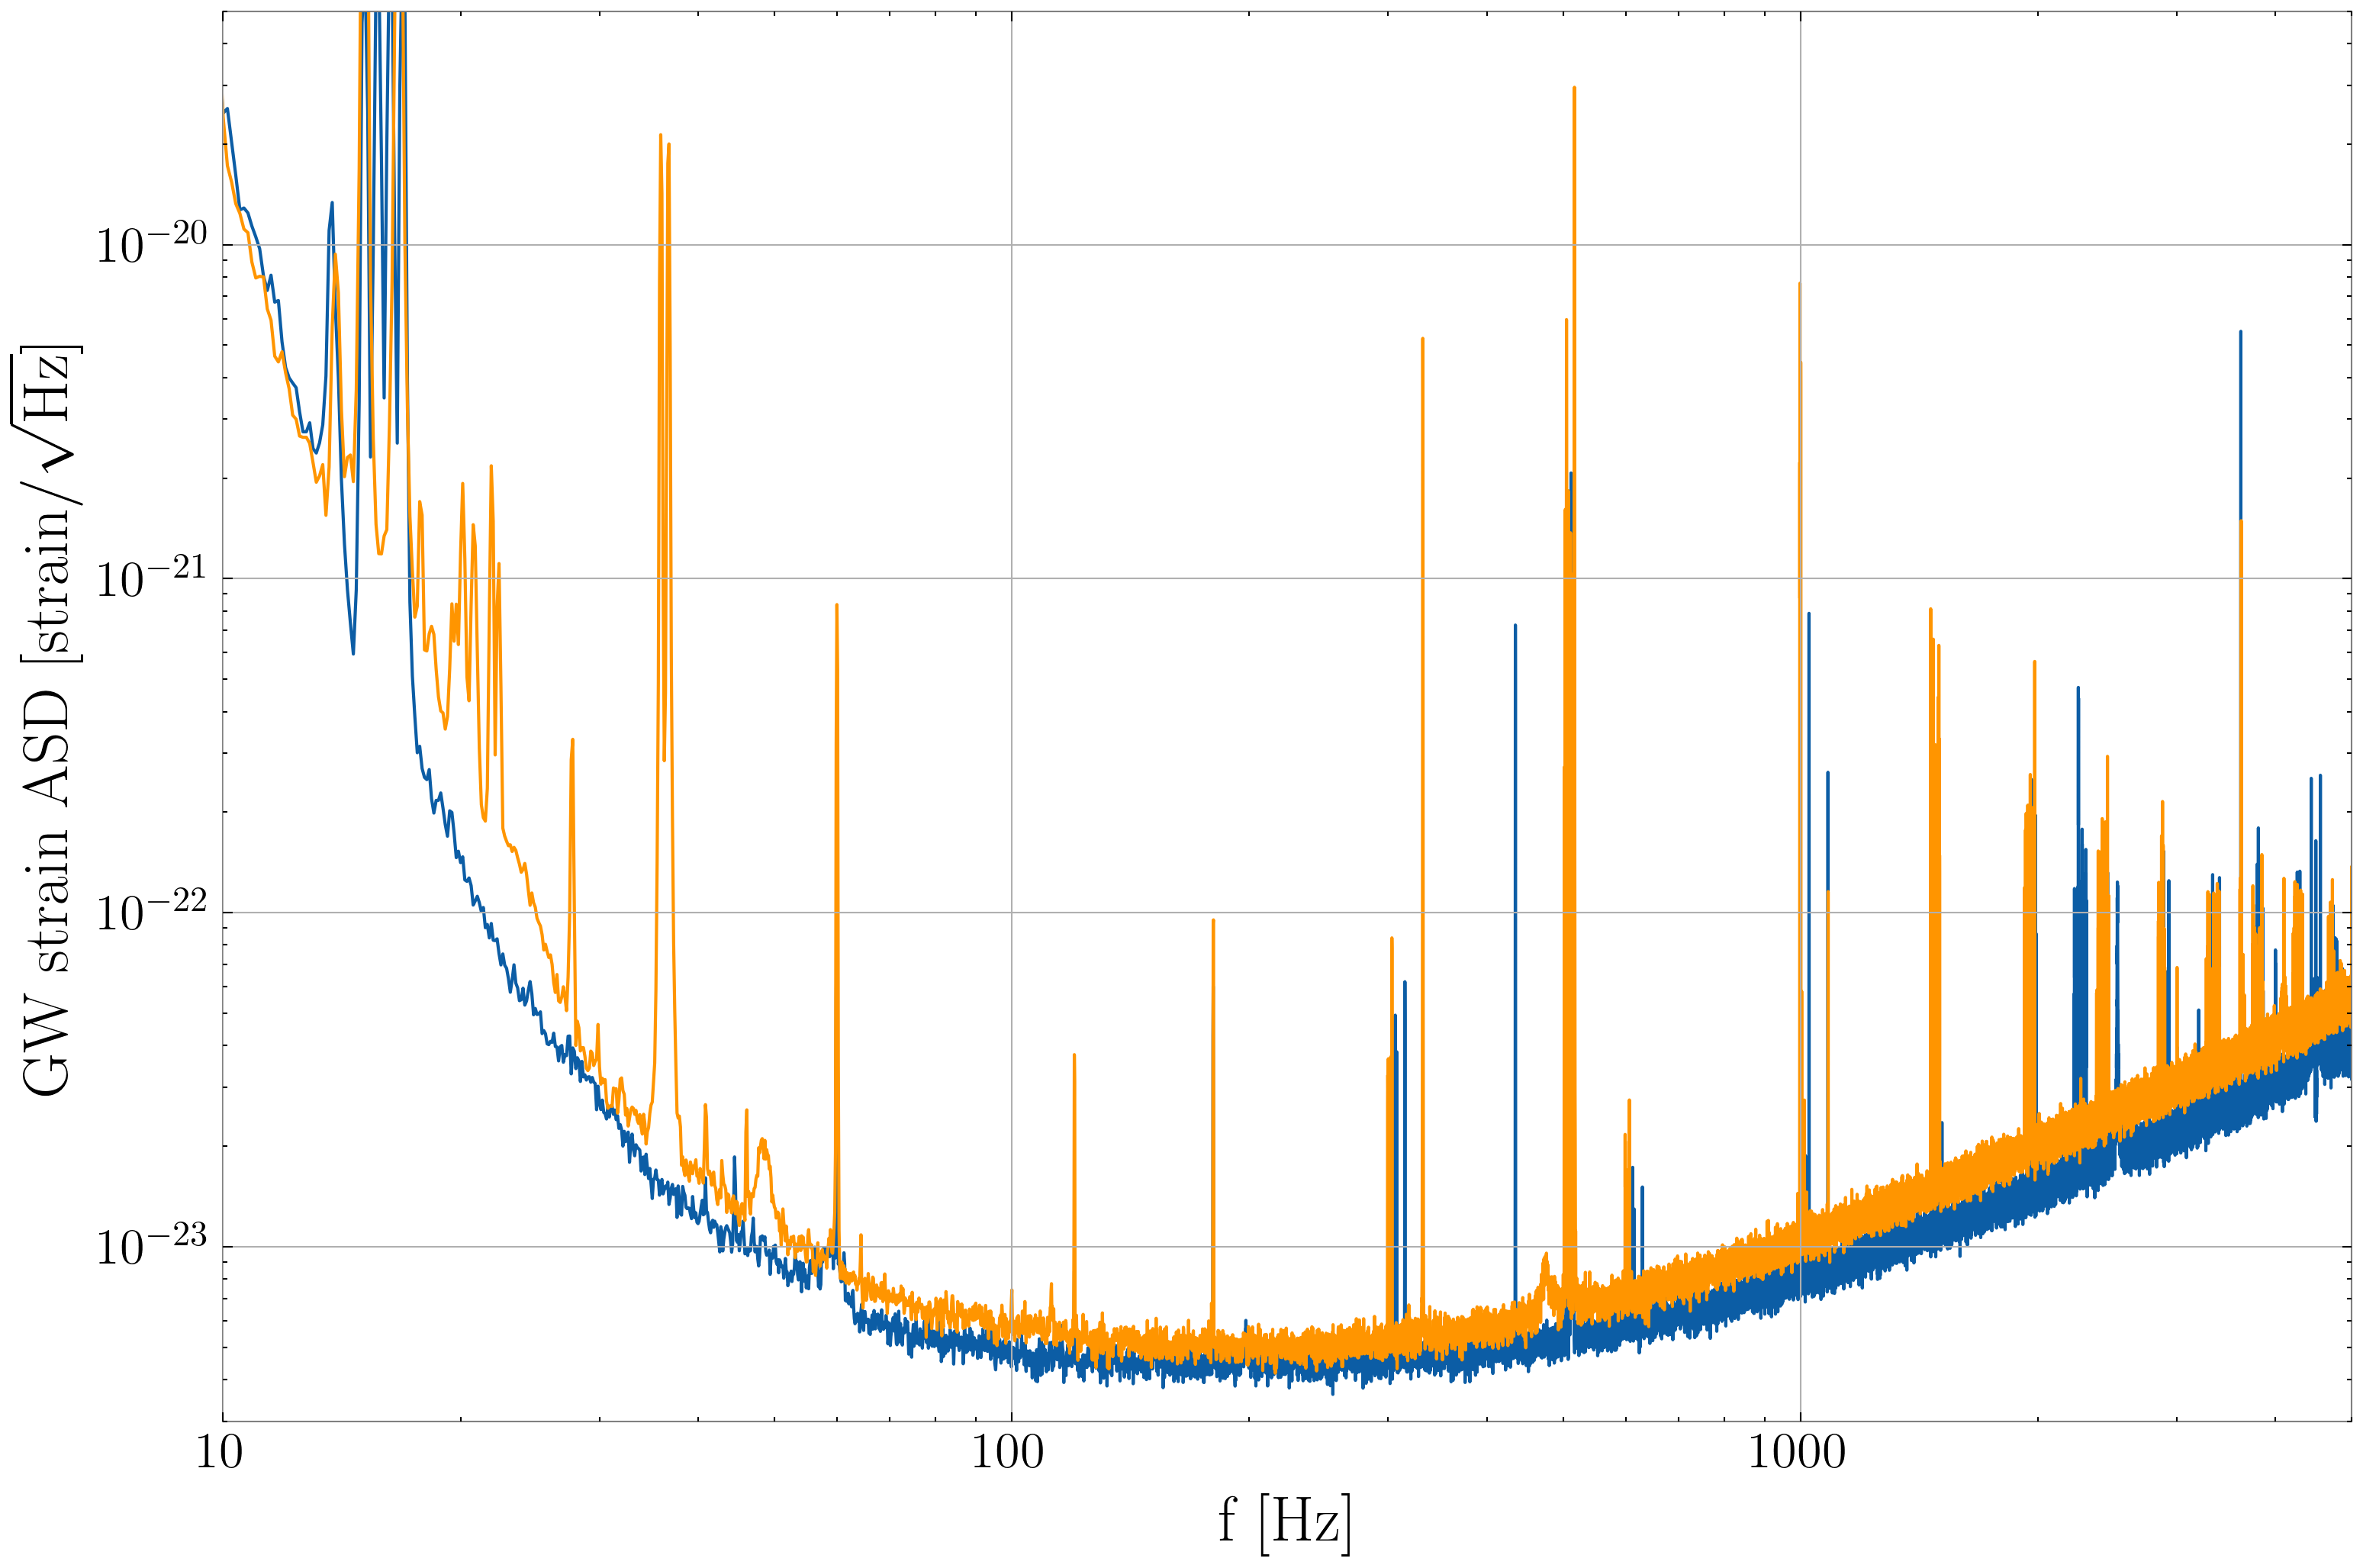
\includegraphics[width=\columnwidth]{images/sensitivity}
	\end{center}
	\caption{Sensitivity plot for LIGO-Hanford (orange) and LIGO-Livingston (blue) for a snapshot of data (\DIFdelbeginFL \DIFdelFL{$\sim 10$ }\DIFdelendFL \DIFaddbeginFL \DIFaddFL{$10.0$ }\DIFaddendFL minutes) from O3 (channel \texttt{*:DCS-CALIB\_STRAIN\_C01\_AR}, see Ref.~\cite{LIGO_O3, GWOSC:online}. The \DIFaddbeginFL \DIFaddFL{vertical axis plots the amplitude }\DIFaddendFL spectral \DIFaddbeginFL \DIFaddFL{density of the detector noise in units of Hz $^{-1/2}$, while the horizontal axis plots the observation frequency in units of Hz. The spectral }\DIFaddendFL line at $60\,{\rm Hz}$ is clearly visible \DIFaddbeginFL \DIFaddFL{as a spike rising three decades}\DIFaddendFL , along with multiple other instrumental lines at other frequencies.}\label{fig:strainSensitivity}
\end{figure}
\begin{figure}
	\DIFdelbeginFL %DIFDELCMD < 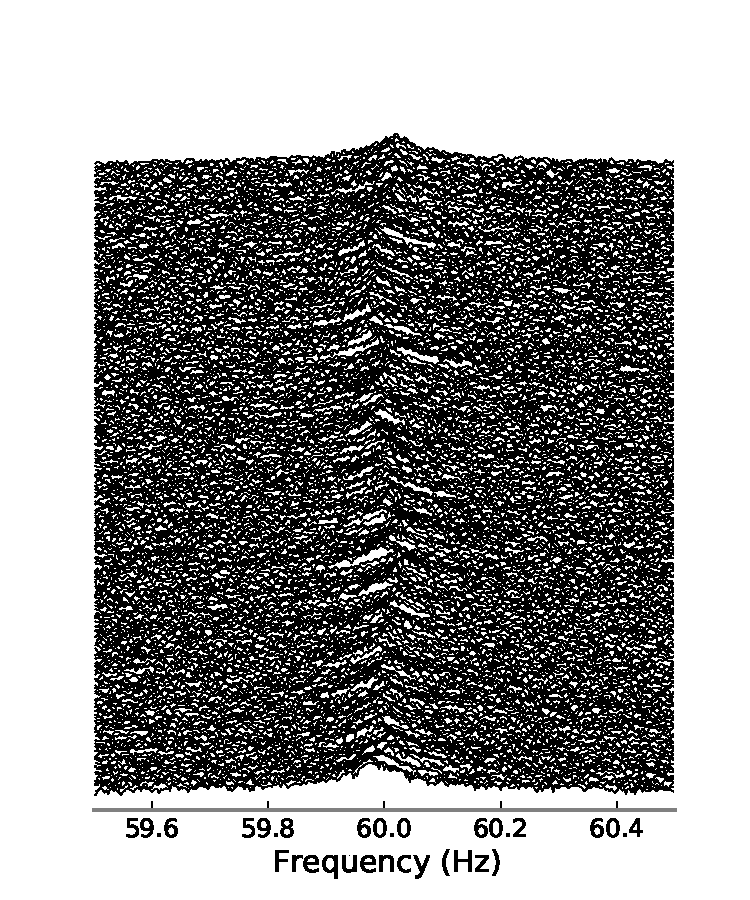
\includegraphics[width=\columnwidth]{images/powerCascade}
%DIFDELCMD < 	%%%
\DIFdelendFL \DIFaddbeginFL 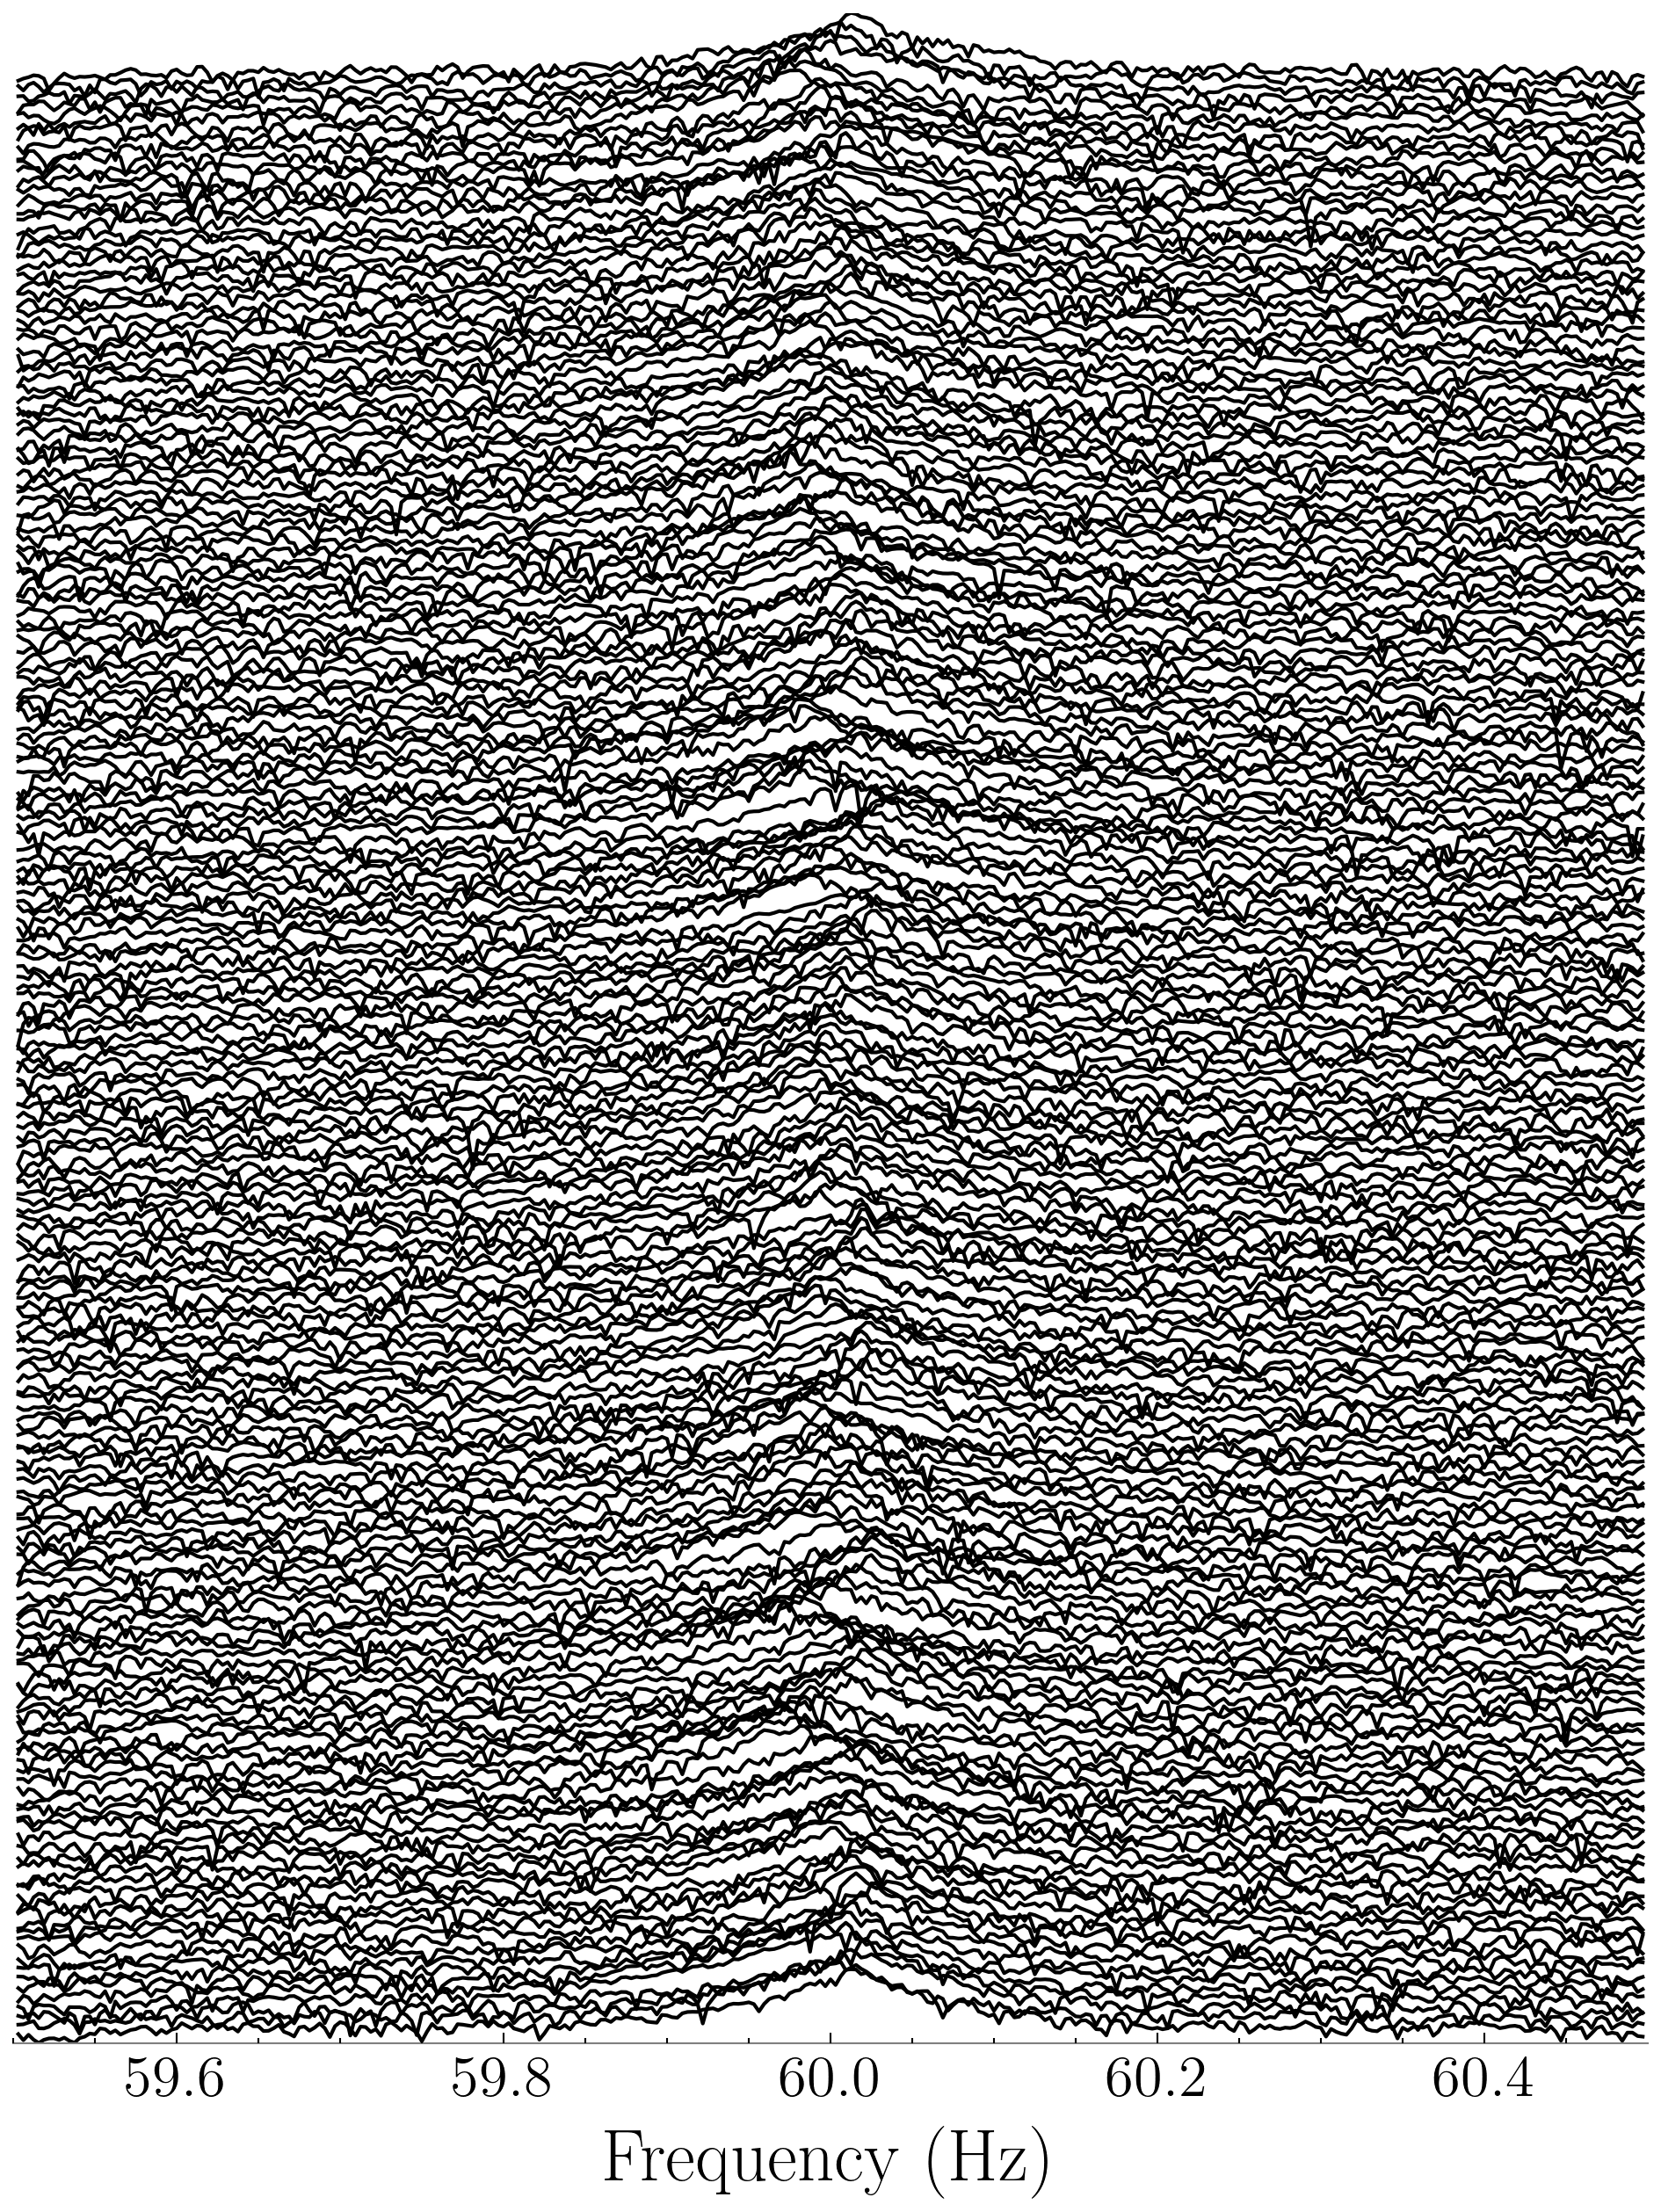
\includegraphics[width=\columnwidth]{images/new_cascade_O3_new}
	\DIFaddendFL \caption{Cascade plot showing the \DIFaddbeginFL \DIFaddFL{temporal evolution of the }\DIFaddendFL amplitude spectral density \DIFaddbeginFL \DIFaddFL{(units: Hz$^{-1/2}$) }\DIFaddendFL of the \DIFdelbeginFL \DIFdelFL{Hanford }\DIFdelendFL \DIFaddbeginFL \DIFaddFL{LIGO-Hanford mains-power }\DIFaddendFL PEM monitor \CSOneName~ (corner station, phase 1) \DIFdelbeginFL \DIFdelFL{over time}\DIFdelendFL \DIFaddbeginFL \DIFaddFL{as a function of frequency (units: Hz)}\DIFaddendFL . Each trace corresponds to $320\,{\rm s}$ ($\approx 5\,{\rm min}$) of data ($210$ \DIFdelbeginFL \DIFdelFL{lines plotted}\DIFdelendFL \DIFaddbeginFL \DIFaddFL{traces stacked vertically}\DIFaddendFL ). The \DIFdelbeginFL \DIFdelFL{wandering }\DIFdelendFL \DIFaddbeginFL \DIFaddFL{peak }\DIFaddendFL of the \DIFdelbeginFL \DIFdelFL{60Hz instrumental }\DIFdelendFL \DIFaddbeginFL \DIFaddFL{mains power $60 \, {\rm Hz}$ }\DIFaddendFL line \DIFaddbeginFL \DIFaddFL{wanders by $\approx \pm 30$ mHz }\DIFaddendFL about its \DIFdelbeginFL \DIFdelFL{central value can be seen}\DIFdelendFL \DIFaddbeginFL \DIFaddFL{time-averaged frequency}\DIFaddendFL .}
	\label{fig:powerCascade}
\end{figure}
% the script for this plot is here on CIT
%/home/hannah.middleton/repositories/powerlines/powergridlines/plots/asd




%DIF > 
\DIFaddbegin 










\DIFaddend %At each detector there are nine PEM for the power grid monitoring all three phases of power at the corner and two end stations at a sample rate of $1024\,{\rm Hz}$. 
%https://arxiv.org/abs/1903.03866 useful for Jaranowski discussion
\subsection{Statement of the problem: signal and noise models}  \label{sec21}
Let $x(t)$ denote the scalar time series output by the \DIFdelbegin \DIFdel{``science" or }\DIFdelend \DIFaddbegin \DIFadd{GW }\DIFaddend strain channel of a LIGO-like long baseline interferometer. Suppose that $x(t)$ is sampled at discrete times $t_n$, with $1 \leq n \leq N$ and uniform sampling interval $\Delta t = t_n - t_{n-1}$. Let $r(t)$ denote the scalar time series output by the environmental \DIFaddbegin \DIFadd{reference }\DIFaddend channel relevant for filtering interference; here $r(t)$ is of one of the three phases of mains power measured at some reference point in the detector. The reference signal is usually sampled less frequently than $x(t)$ at discrete times $t_{n_k}$, with $1 \leq k \leq K$ and $1 \leq n_k \leq N$. We assume for the sake of convenience that every $t_{n_k}$ coincides with some $t_n$ for all $k$, but the condition is not essential. \newline 

The strain channel is composed of a gravitational wave signal $h(t)$, \DIFdelbegin \DIFdel{non Gaussian }\DIFdelend \DIFaddbegin \DIFadd{non-Gaussian }\DIFaddend interference $c(t)$ (sometimes called ``clutter") and Gaussian noise $n(t)$ in a linear combination\DIFdelbegin \DIFdel{:
}\DIFdelend \DIFaddbegin \DIFadd{,
}\DIFaddend \begin{eqnarray}
	x(t) = h(t) + c(t) + n(t) \ .
	\label{eq:data}
\end{eqnarray}
 In this paper the gravitational wave signal takes the form predicted by \citet{Jaranowski1998} for a biaxial rotor, e.g. a neutron star (NS) emitting \DIFdelbegin \DIFdel{continuous }\DIFdelend gravitational waves at multiples of the star\DIFaddbegin \DIFadd{'s }\DIFaddend spin frequency $f_{\star}$. The GW signal is \DIFdelbegin \DIFdel{quasimonchromatic}\DIFdelend \DIFaddbegin \DIFadd{quasi-monochromatic}\DIFaddend , amplitude-modulated by the rotation of the Earth and \DIFdelbegin \DIFdel{frequency modulated }\DIFdelend \DIFaddbegin \DIFadd{frequency-modulated }\DIFaddend by the Earth's orbital motion. The noise $n(t)$ is white with $\langle n(t_n) n(t_{n'})\rangle = \sigma_n^2 \delta_{n n'}$. Noise samples $n(t_n)$ are drawn from a Gaussian distribution with zero mean and variance $\sigma_n^2$. The interference \DIFdelbegin \DIFdel{clutter }\DIFdelend $c(t)$ takes a form determined by instrumental processes but is generally a long-lived\DIFdelbegin \DIFdel{narrow }\DIFdelend \DIFaddbegin \DIFadd{, narrowband }\DIFaddend spectral feature. We \DIFdelbegin \DIFdel{can }\DIFdelend relate $c(t)$ to the \DIFdelbegin \DIFdel{instrumental }\DIFdelend \DIFaddbegin \DIFadd{mains }\DIFaddend voltage $r(t)$ in \DIFdelbegin \DIFdel{the following}\DIFdelend \DIFaddbegin \DIFadd{this paper}\DIFaddend . \newline 

 
 Mains power is characterized by three properties. First, the frequency is maintained at a constant value across the grid to \DIFdelbegin \DIFdel{to }\DIFdelend a good approximation by internal grid mechanisms (effectively a phase locked loop), with central frequency $f_{\rm ac} = 60$ Hz in North America. A slow periodic modulation occurs around $f_{\rm ac}$ with a small amplitude $\Delta f_{\rm ac} \lesssim 0.5$ Hz and period $P$\DIFaddbegin \DIFadd{, }\DIFaddend which wanders randomly and uniformly in the range $0 \leq P \leq P_{\rm max}$. \DIFdelbegin \DIFdel{Secondly}\DIFdelend \DIFaddbegin \DIFadd{Second}\DIFaddend , the phase \DIFaddbegin \DIFadd{offset }\DIFaddend $\Theta(t)$ of the voltage $r(t)$ wanders stochastically. We assume that the phase noise is white and Gaussian, with $n_{\Theta}(t_n)$ drawn from a Gaussian distribution with zero mean and variance $\sigma_{\Theta}^2$, \DIFdelbegin \DIFdel{and }\DIFdelend \DIFaddbegin \DIFadd{i.e. }\DIFaddend $\langle n_{\Theta} (t_n) n_{\Theta} (t_{n'})\rangle = \sigma^2_{\Theta} \delta_{n n'}$. Third, the voltage amplitude, $A_r(t)$, is random. We assume that samples $A_r(t)$ are distributed uniformly within $[A_{\rm ac} - \Delta A_{\rm ac} , A_{\rm ac} + \Delta A_{\rm ac}]$. We can then write the reference voltage as,
 \begin{eqnarray}
 	r(t) = A_r(t_n) \cos \left[ 2 \pi f_{\rm ac} t + \Theta(t)\right] +n_r(t_n) \ ,
 	\label{eq:voltage}
 \end{eqnarray}
with
 \begin{eqnarray}
\Theta(t) = 2 \pi \Delta f_{\rm ac} \cos\DIFdelbegin %DIFDELCMD < \left(%%%
\DIFdelend \DIFaddbegin \left[\DIFaddend \frac{2 \pi t}{P(t_n)}\DIFdelbegin %DIFDELCMD < \right) %%%
\DIFdelend \DIFaddbegin \right] \DIFaddend + n_{\Theta} (t_n) \ ,
\label{eq:voltage_theta}
\end{eqnarray}
%\begin{align}
%	r(t) &= \nonumber \\
%	& A_r(t_n) \cos \left( 2 \pi f_{\rm ac} t + 2 \pi \Delta f_{\rm ac} \cos\left(\frac{2 \pi t}{P(t_n)}\right) + n_{\Theta} (t_n)\right) \nonumber \\
%	& +w(t_n)
%	\label{eq:voltage}
%\end{align}
for $t_n \leq t \leq t_{n+1}$. That is, at time $t_n$, random variables \DIFdelbegin \DIFdel{$A_t(t_n)$}\DIFdelend \DIFaddbegin \DIFadd{$A_r(t_n)$}\DIFaddend , $P(t_n)$ and $n_{\Theta} (t_n)$ are drawn from the distribution $\mathcal{U}[A_{\rm ac} - \Delta A_{\rm ac},A_{\rm ac} + \Delta A_{\rm ac} ]$, $\mathcal{U}[0, P_{\rm max}]$, and $\mathcal{N} [0, \sigma_{\Theta}^2]$ respectively. Equation \eqref{eq:voltage} then \DIFdelbegin \DIFdel{runs forward over an interval of length }\DIFdelend \DIFaddbegin \DIFadd{steps forward over a time interval }\DIFaddend $\Delta t$\DIFdelbegin \DIFdel{. Hence }\DIFdelend \DIFaddbegin \DIFadd{; that is, }\DIFaddend $r(t)$ is discontinuous \DIFdelbegin \DIFdel{at each sampling time }\DIFdelend \DIFaddbegin \DIFadd{from one time step to the next due to random sampling}\DIFaddend . In Equation \eqref{eq:voltage}, $n_r(t_n)$ is the reference signal measurement noise at $t_n$, assumed to be white and Gaussian with \DIFdelbegin \DIFdel{$r_r(t_n)$ }\DIFdelend \DIFaddbegin \DIFadd{$n_r(t_n)$ }\DIFaddend drawn from a Gaussian with zero mean and variance $\sigma_r^2$. All the white measurement and process noises are assumed \DIFaddbegin \DIFadd{to be }\DIFaddend independent. \newline 

Mains power couples into the strain channel in various complicated ways, e.g. through electronic devices, or inductively through ambient magnetic fields. A central assumption in this work is that the interference in the strain channel is an exact, amplitude-scaled replica of the reference signal up to a delay $\tau_{\rm delay}$ which is attributed to spatial propagation \DIFdelbegin \DIFdel{effects between the reference measurement front and the interferometer mirrors or dark front}\DIFdelend \DIFaddbegin \DIFadd{between the PEM site and the GW-sensing apparatus}\DIFaddend . Hence we can express the interference \DIFdelbegin \DIFdel{clutter as, 
 }\begin{eqnarray*}
	\DIFdel{c(t) = A_c(t'_n) \cos \left[ 2 \pi f_{\rm ac} t' + \Theta(t')\right] \ ,
	%DIFDELCMD < \label{eq:vclutter}%%%
}\end{eqnarray*}%DIFAUXCMD
\DIFdelend \DIFaddbegin \DIFadd{as, 
 }\begin{align}
	\DIFadd{c(t) = A_c(t_n - \tau_{\rm delay}) \cos \biggl [ }& \DIFadd{2 \pi f_{\rm ac} (t_n - \tau_{\rm delay}) \nonumber }\\ 
	&\DIFadd{+ \Theta(t_n - \tau_{\rm delay}	) \biggr ] \ ,
	\label{eq:vclutter}
}\end{align}\DIFaddend 
for $t_n \leq t \leq t_{n+1}$\DIFdelbegin \DIFdel{and $t' = t_n - \tau_{\rm delay}$}\DIFdelend . The amplitude $A_c$ is distributed as \DIFdelbegin \DIFdel{$\mathcal{U}[A_{\rm ac} ,A_{\rm ac} + \Delta A_{\rm ac} ]$}\DIFdelend \DIFaddbegin \DIFadd{$\mathcal{U}[A_{\rm ac}- \Delta A_{\rm ac} ,A_{\rm ac} + \Delta A_{\rm ac} ]$}\DIFaddend . For this work we consider $0 \leq \tau_{\rm delay} \leq 10 \Delta t$, but wider or narrower ranges \DIFdelbegin \DIFdel{is }\DIFdelend \DIFaddbegin \DIFadd{are }\DIFaddend possible and straightforward to \DIFdelbegin \DIFdel{be implemented. The assumptions of an exact replica between the interference and the reference }\DIFdelend \DIFaddbegin \DIFadd{implement. The assumption that $c(t)$ is a scaled replica of $r(t)$ }\DIFaddend is tested in \DIFdelbegin \DIFdel{the following section.
}\footnote{%DIFDELCMD < \tiny %%%
\DIFdel{\textcolor{red}{TK: Why are the amplitudes of $A_r$ and $A_c$ distributed differently?}}%DIFDELCMD < \normalsize%%%
}
%DIFAUXCMD
\addtocounter{footnote}{-1}%DIFAUXCMD
\DIFdelend \DIFaddbegin \DIFadd{Section \ref{sec23}.
}\DIFaddend 




\subsection{\DIFdelbegin \DIFdel{Cross-correlating the interference }\DIFdelend \DIFaddbegin \DIFadd{Coherence between $x(t)$ }\DIFaddend and \DIFdelbegin \DIFdel{reference}\DIFdelend \DIFaddbegin \DIFadd{$r(t)$}\DIFaddend }  \label{sec23}
A key assumption \DIFdelbegin \DIFdel{of the construction }\DIFdelend in Section \ref{sec21} is that the 60 Hz \DIFdelbegin \DIFdel{noise that is }\DIFdelend \DIFaddbegin \DIFadd{interference }\DIFaddend recorded in the reference PEM channel is also present in the \DIFdelbegin \DIFdel{LIGO }\DIFdelend strain channel. That is, the \DIFdelbegin \DIFdel{noise recorded in the PEM channel }\DIFdelend \DIFaddbegin \DIFadd{mains voltage recorded by the PEM }\DIFaddend is imprinted onto the strain channel \DIFaddbegin \DIFadd{up to a proportionality constant and time delay}\DIFaddend . In order to test this assumption we \DIFdelbegin \DIFdel{cross-correlate the }\DIFdelend \DIFaddbegin \DIFadd{calculate the coherence between the }\DIFaddend strain channel and the PEM channel. \DIFdelbegin \DIFdel{If there is a noise signal at 60 Hz present in both channels then it should be revealed by this cross-correlation. We use open sourced }\DIFdelend \DIFaddbegin \newline 

\DIFadd{The coherence between two time series $x(t)$ and $r(t)$ is given by 
}\begin{equation}
	\DIFadd{C_{xr}(f)	= \frac{|P_{xr}(f)|^2}{P_{xx}(f) P_{rr}(f)}  \label{eq:coherence}
}\end{equation}
\DIFadd{where $f$ is the frequency, $P_{xr}$ is the (cross) power spectral density and $ 0 \leq C_{xr}(f) \leq 1$. $C_{xr}(f) = 0$ indicates that the two signals are completely unrelated, whilst $C_{xr}(f) = 1$ indicates that the two signals have an ideal, noiseless, linear relationship i.e. $x(t) = g(t) \ast r(t)$ for impulse response function $g(t)$.  If $ 0 < C_{xr}(f) < 1$ then this indicates that the relationship between $x(t)$ and $r(t)$ is non-linear, either due to measurement noise or else contributions to $x(t)$ from additional signals. Heuristically, for linear systems, $C_{xr}(f)$ can be understood as the fraction of the power in $x(t)$ that is produced by $r(t)$, at $f$. }\newline 


\DIFadd{We use }\DIFaddend data for the strain and PEM channels from the first part of the third LIGO observing run, O3a \cite{LIGO_O3}. \DIFdelbegin \DIFdel{This data is }\DIFdelend \DIFaddbegin \DIFadd{These data are }\DIFaddend obtained via the \DIFdelbegin \DIFdel{Gravitational Wave
Open Science Center }\DIFdelend \DIFaddbegin \DIFadd{LIGO Data Grid  }\DIFaddend \footnote{\DIFdelbegin %DIFDELCMD < \url{gwosc.org}%%%
\DIFdelend \DIFaddbegin \url{https://computing.docs.ligo.org/guide/computing-centres/ldg/}\DIFaddend } using the \texttt{GWPy} package \cite{gwpy}. In \DIFdelbegin \DIFdel{the auxiliary }\DIFdelend O3a \DIFdelbegin \DIFdel{data there are 9 }\DIFdelend \DIFaddbegin \DIFadd{there are nine independent }\DIFaddend PEM channels at \DIFaddbegin \DIFadd{both }\DIFaddend LIGO-Livingston and \DIFdelbegin \DIFdel{7 PEM channels at }\DIFdelend LIGO-Hanford \DIFaddbegin \DIFadd{that directly measure the mains voltage }\DIFaddend \footnote{\DIFdelbegin %DIFDELCMD < \url{https://git.ligo.org/gwosc/tutorials/gwosc-aux-tutorials/-/tree/main/Channels}%%%
\DIFdelend \DIFaddbegin \url{https://git.ligo.org/detchar/ligo-channel-lists/-/blob/master/O3/L1-O3-pem.ini}\DIFaddend }. \DIFdelbegin \DIFdel{For this work }\DIFdelend \DIFaddbegin \DIFadd{In this paper }\DIFaddend we consider just the LIGO-Livingston data\DIFdelbegin \DIFdel{. }\DIFdelend \DIFaddbegin \DIFadd{, as they suffice to make the point. Specifically, there are 3 PEM mains voltage monitors in the electronics bay in each of the X-arm end station (}\texttt{\DIFadd{EX}}\DIFadd{), the Y-arm end station (}\texttt{\DIFadd{EY}}\DIFadd{) and the corner station (}\texttt{\DIFadd{CS}}\DIFadd{). Each of the three PEMs at each station measures a separate component of three-phase mains power. }\DIFaddend The strain data \DIFdelbegin \DIFdel{is obtained at a rate of }\DIFdelend \DIFaddbegin \DIFadd{are sampled at }\DIFaddend 16384 Hz and downsampled to \DIFdelbegin \DIFdel{4096 }\DIFdelend \DIFaddbegin \DIFadd{1024 }\DIFaddend Hz to match the sampling rate of the PEM channels. \DIFdelbegin \DIFdel{In Figure \ref{correlation_2} we show the coherence between each of the 9 PEM channels and the }\DIFdelend \DIFaddbegin \newline 
%DIF > https://arxiv.org/pdf/1812.05225.pdf

\DIFadd{Figure \ref{coherenceplot_1} displays $C_{xr}(f)$ between the }\DIFaddend high latency, calibrated strain channel \texttt{L1:DCS-CALIB\_STRAIN\_C01\_AR} \DIFaddbegin \DIFadd{and each of the nine reference PEM channels }\DIFaddend over a 10 minute \DIFdelbegin \DIFdel{time period}\DIFdelend \DIFaddbegin \DIFadd{interval}\DIFaddend . For all channels there is a clear \DIFdelbegin \DIFdel{coherence feature at 60Hz. The coherence feature is typically large, with values $> 0.5$ for 7 of the 9 PEM channels. Compared to the other channels, the coherence is particularly weak for the channels }\texttt{\DIFdel{L1:PEM-EY\_MIC\_VEA\_PLUSY\_DQ}} %DIFAUXCMD
\DIFdelend \DIFaddbegin \DIFadd{spike in the $C_{xr}(f)$ at 60 Hz, with a mean amplitude $=0.85$ (unitless). }\newline 

 \DIFadd{It is important to note that whilst $C_{xr}(f=60 \text{Hz})$ between $x(t)$ }\DIFaddend and \DIFdelbegin \texttt{\DIFdel{L1:PEM-CS\_MIC\_LVEA\_INPUTOPTICS\_DQ}}%DIFAUXCMD
\DIFdel{. These channels corresponds to microphone PEMs in the LIGO vacuum equipment area and so would be less sensitive to the 60Hz noise than e.g. }\texttt{\DIFdel{L1:PEM-EY\_MAINSMON\_EBAY\_1\_DQ}} %DIFAUXCMD
\DIFdel{which directly measures the voltage. In Figure \ref{correlation_1} we also show }\DIFdelend \DIFaddbegin \DIFadd{$r(t)$ is strong, it is also time variable. Figure \ref{correlation_1} displays }\DIFaddend the coherence spectrogram\DIFaddbegin \DIFadd{, }\DIFaddend i.e. the time-varying coherence\DIFaddbegin \DIFadd{, }\DIFaddend between the strain channel and the PEM channel \PEMChanName \DIFdelbegin \DIFdel{.  The coherence is calculated across }\DIFdelend \DIFaddbegin \DIFadd{\, (c.f. top panel, Figure \ref{coherenceplot_1}) over a 1 hour time interval (c.f. the }\DIFaddend 10 \DIFdelbegin \DIFdel{s windows of data. That is , each column of the spectrogram has a width of }\DIFdelend \DIFaddbegin \DIFadd{minute interval of Figure \ref{coherenceplot_1}). $C_{xy}(f)$ is calculated in 10-s blocks; that is, every pixel in Figure \ref{correlation_1} is }\DIFaddend 10 s \DIFdelbegin \DIFdel{. We again observe similar results to Figure \ref{correlation_2} where }\DIFdelend \DIFaddbegin \DIFadd{wide horizontally. We use a Fourier transform window of length 0.5 s, with each window overlapping by 0.25 s (c.f. Welch's method, \mbox{%DIFAUXCMD
\citep{Welch1161901}}\hskip0pt%DIFAUXCMD
). Similar results are observed to Figure \ref{coherenceplot_1}; }\DIFaddend there is a \DIFdelbegin \DIFdel{clear, strong }\DIFdelend \DIFaddbegin \DIFadd{strong coherence (mean value =$0.73$) }\DIFaddend spectral feature at \DIFdelbegin \DIFdel{60Hz. Additional coherence features can also be seen at at $\sim$ 200 Hz and 300 Hz}\DIFdelend \DIFaddbegin \DIFadd{60 Hz which persists across the full 1 hour time interval. However, whilst the feature is persistent, $C_{xr}(f=60 \text{Hz})$ is not constant across the entire interval. Instead it changes in time, with a variance $=0.018$. These variations are evident in the changing colours of the spectrogram at 60 Hz, leading to an apparent ``patchiness" of the line. Additional features in the $C_{xr}(f)$ spectrum are seen near 0.2 kHz and 0.3 kHz}\DIFaddend , corresponding to \DIFdelbegin \DIFdel{different frequency noise }\DIFdelend \DIFaddbegin \DIFadd{instrumental }\DIFaddend lines recorded by the PEM \DIFdelbegin \DIFdel{that also }\DIFdelend \DIFaddbegin \DIFadd{which }\DIFaddend imprint onto the strain channel \DIFaddbegin \DIFadd{and are unrelated to the mains power. Similar results are obtained for the other PEM channels shown in Figure \ref{coherenceplot_1}	. Figures  \ref{coherenceplot_1} and  \ref{correlation_1} justify in part the assumptions in Section \ref{sec21}}\DIFaddend .
\DIFdelbegin \DIFdel{These results showing a strong coherence between the strain and PEM channels demonstrate that our assumptions of Section \ref{sec21}are justified.
}\DIFdelend \begin{figure}
	\begin{center}
		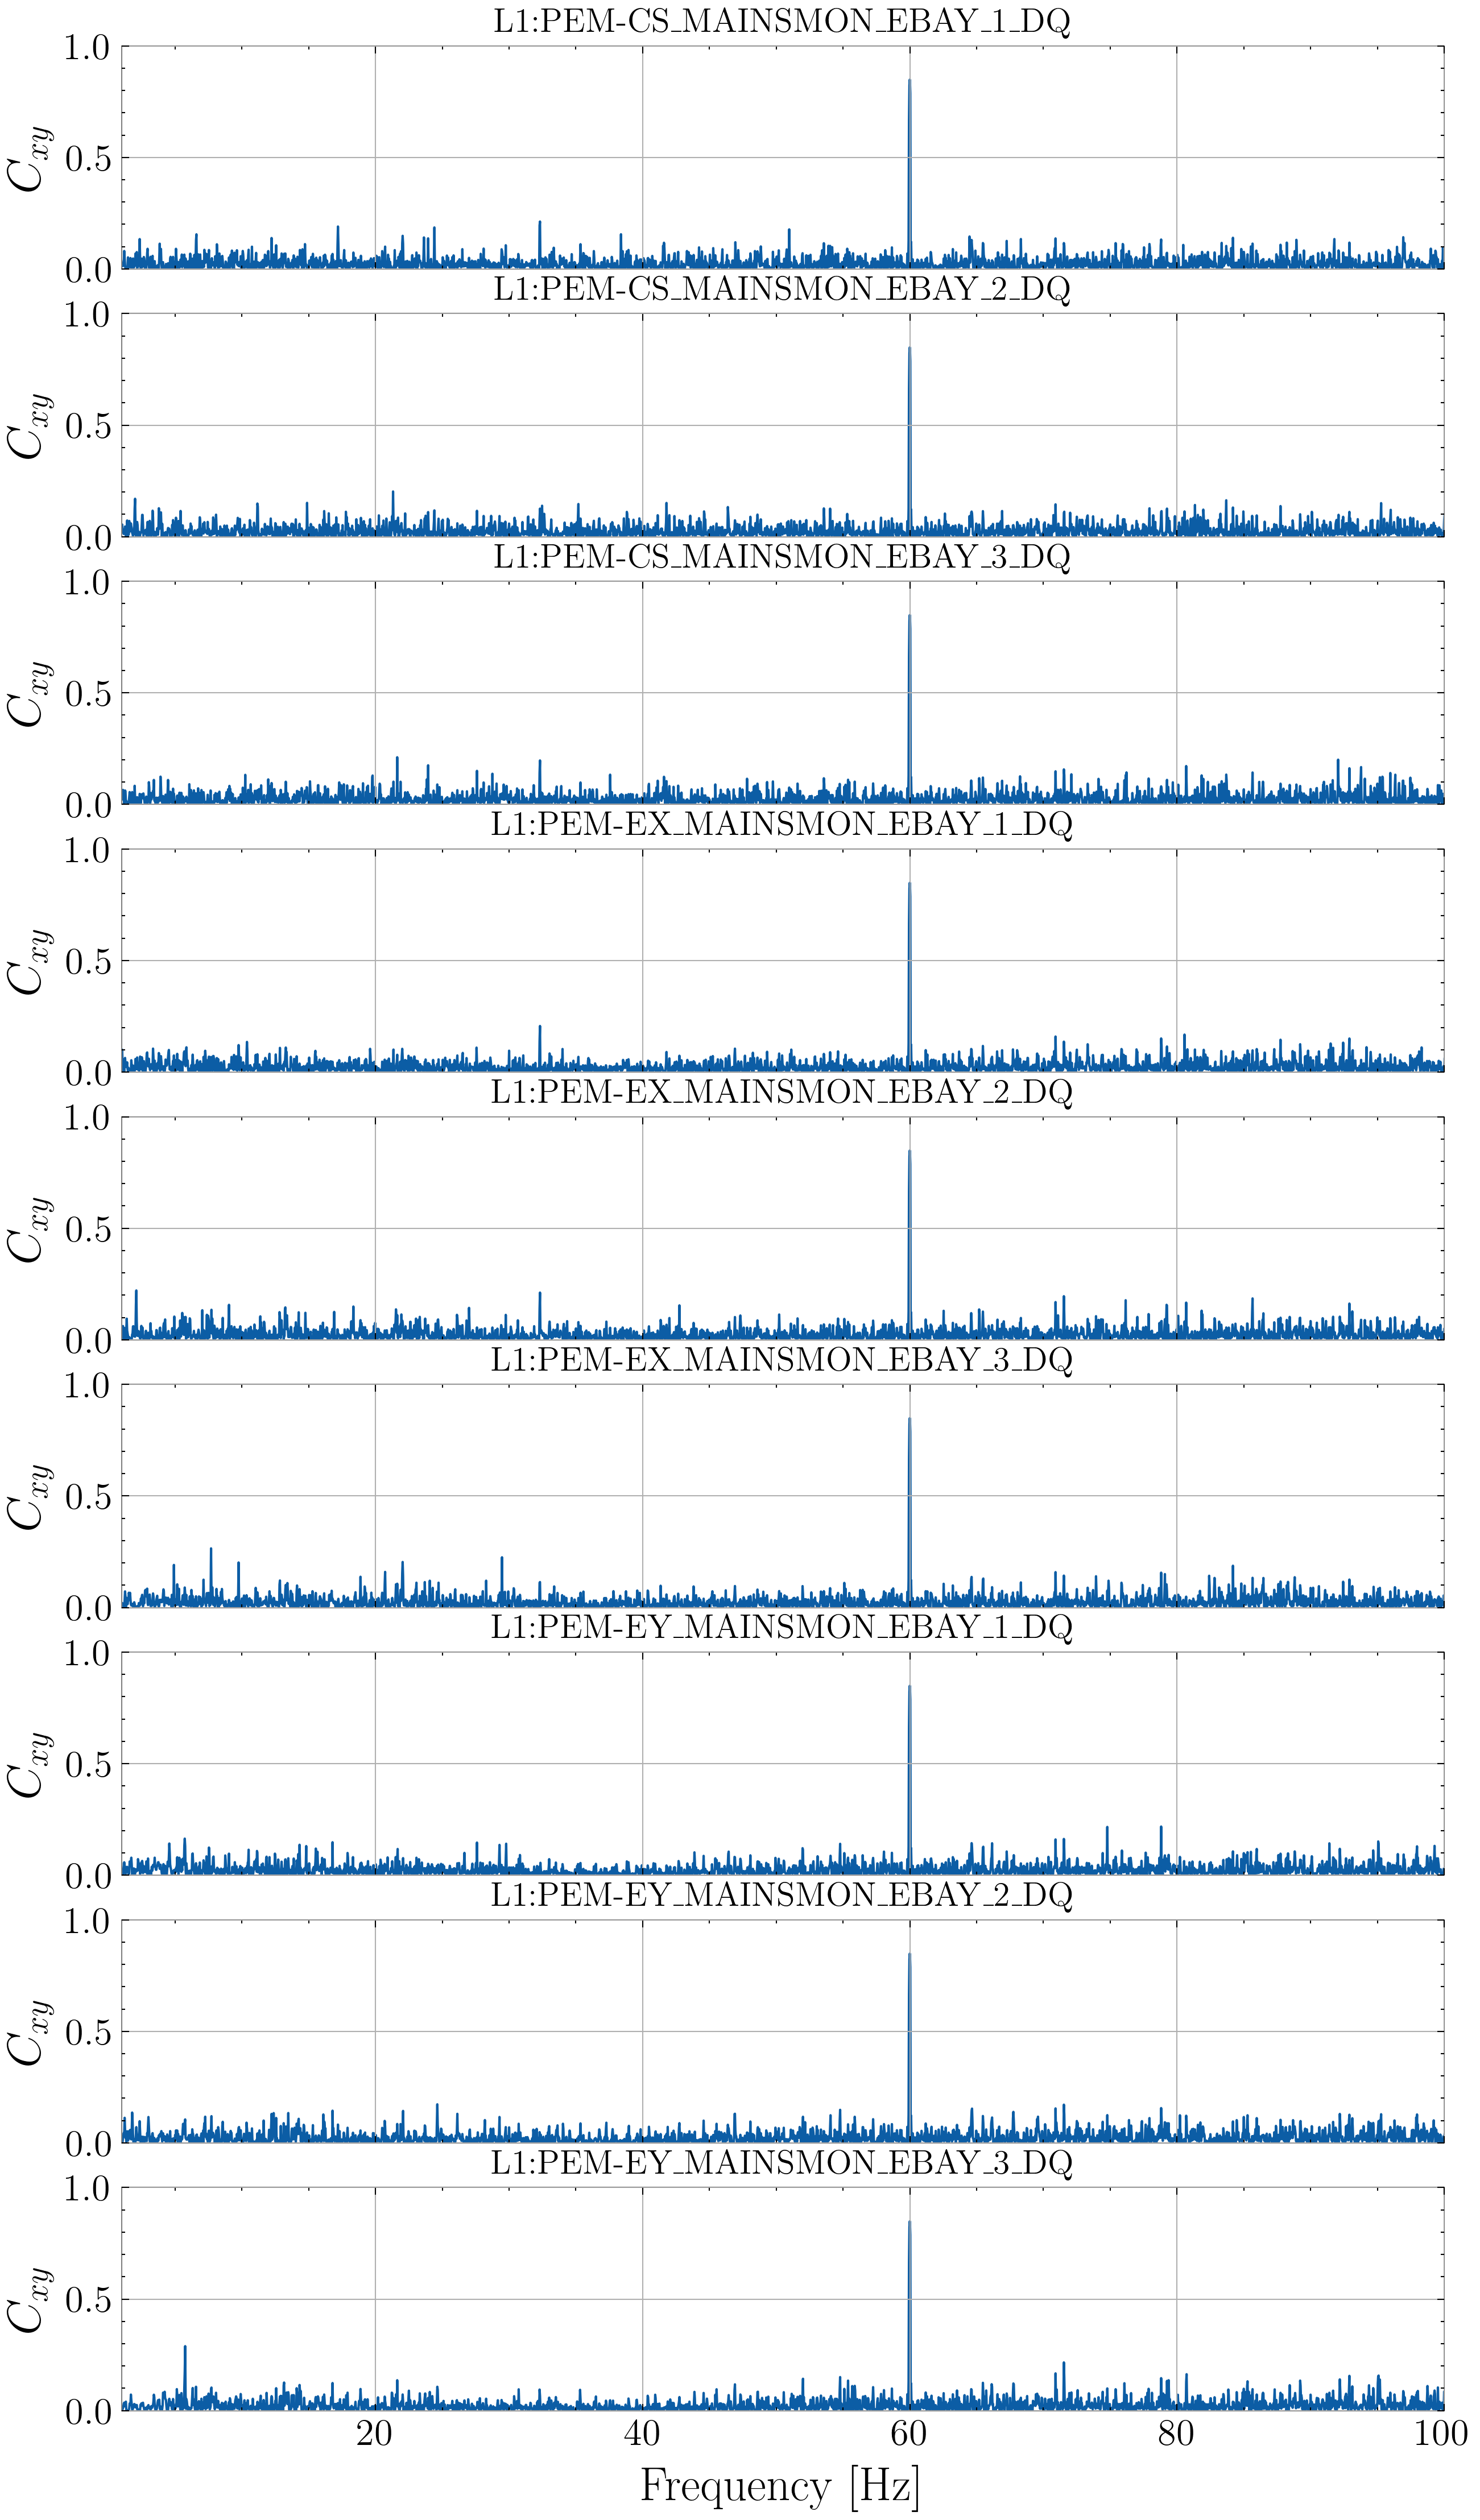
\includegraphics[width=\columnwidth]{images/stacked_coherence_plot}
	\end{center}
	\DIFdelbeginFL %DIFDELCMD < \label{correlation_2}
%DIFDELCMD < 	%%%
\DIFdelendFL \caption{\DIFaddbeginFL \label{coherenceplot_1} \DIFaddendFL Coherence $C_{xy}$\DIFaddbeginFL \DIFaddFL{, defined by Equation \eqref{eq:coherence}, }\DIFaddendFL between the LIGO-Livingston strain channel  \texttt{L1:DCS-CALIB\_STRAIN\_C01\_AR} and the \DIFdelbeginFL \DIFdelFL{9 }\DIFdelendFL \DIFaddbeginFL \DIFaddFL{nine mains-power }\DIFaddendFL PEM channels \DIFdelbeginFL \DIFdelFL{over }\DIFdelendFL \DIFaddbeginFL \DIFaddFL{during }\DIFaddendFL a 10 minute observation \DIFdelbeginFL \DIFdelFL{period}\DIFdelendFL \DIFaddbeginFL \DIFaddFL{interval}\DIFaddendFL . Clear features at 60 Hz are present in \DIFdelbeginFL \DIFdelFL{all of the channels. The coherence is weakest for those PEM channels which do not measure voltage directly}\DIFdelendFL \DIFaddbeginFL \DIFaddFL{every channel}\DIFaddendFL , \DIFdelbeginFL \DIFdelFL{but instead are microphones the the LIGO vacuum equipment area}\DIFdelendFL \DIFaddbeginFL \DIFaddFL{with amplitudes $ > 0.8$ (unitless)}\DIFaddendFL .}
\end{figure}
\begin{figure*}
	\begin{center}
		\DIFdelbeginFL %DIFDELCMD < 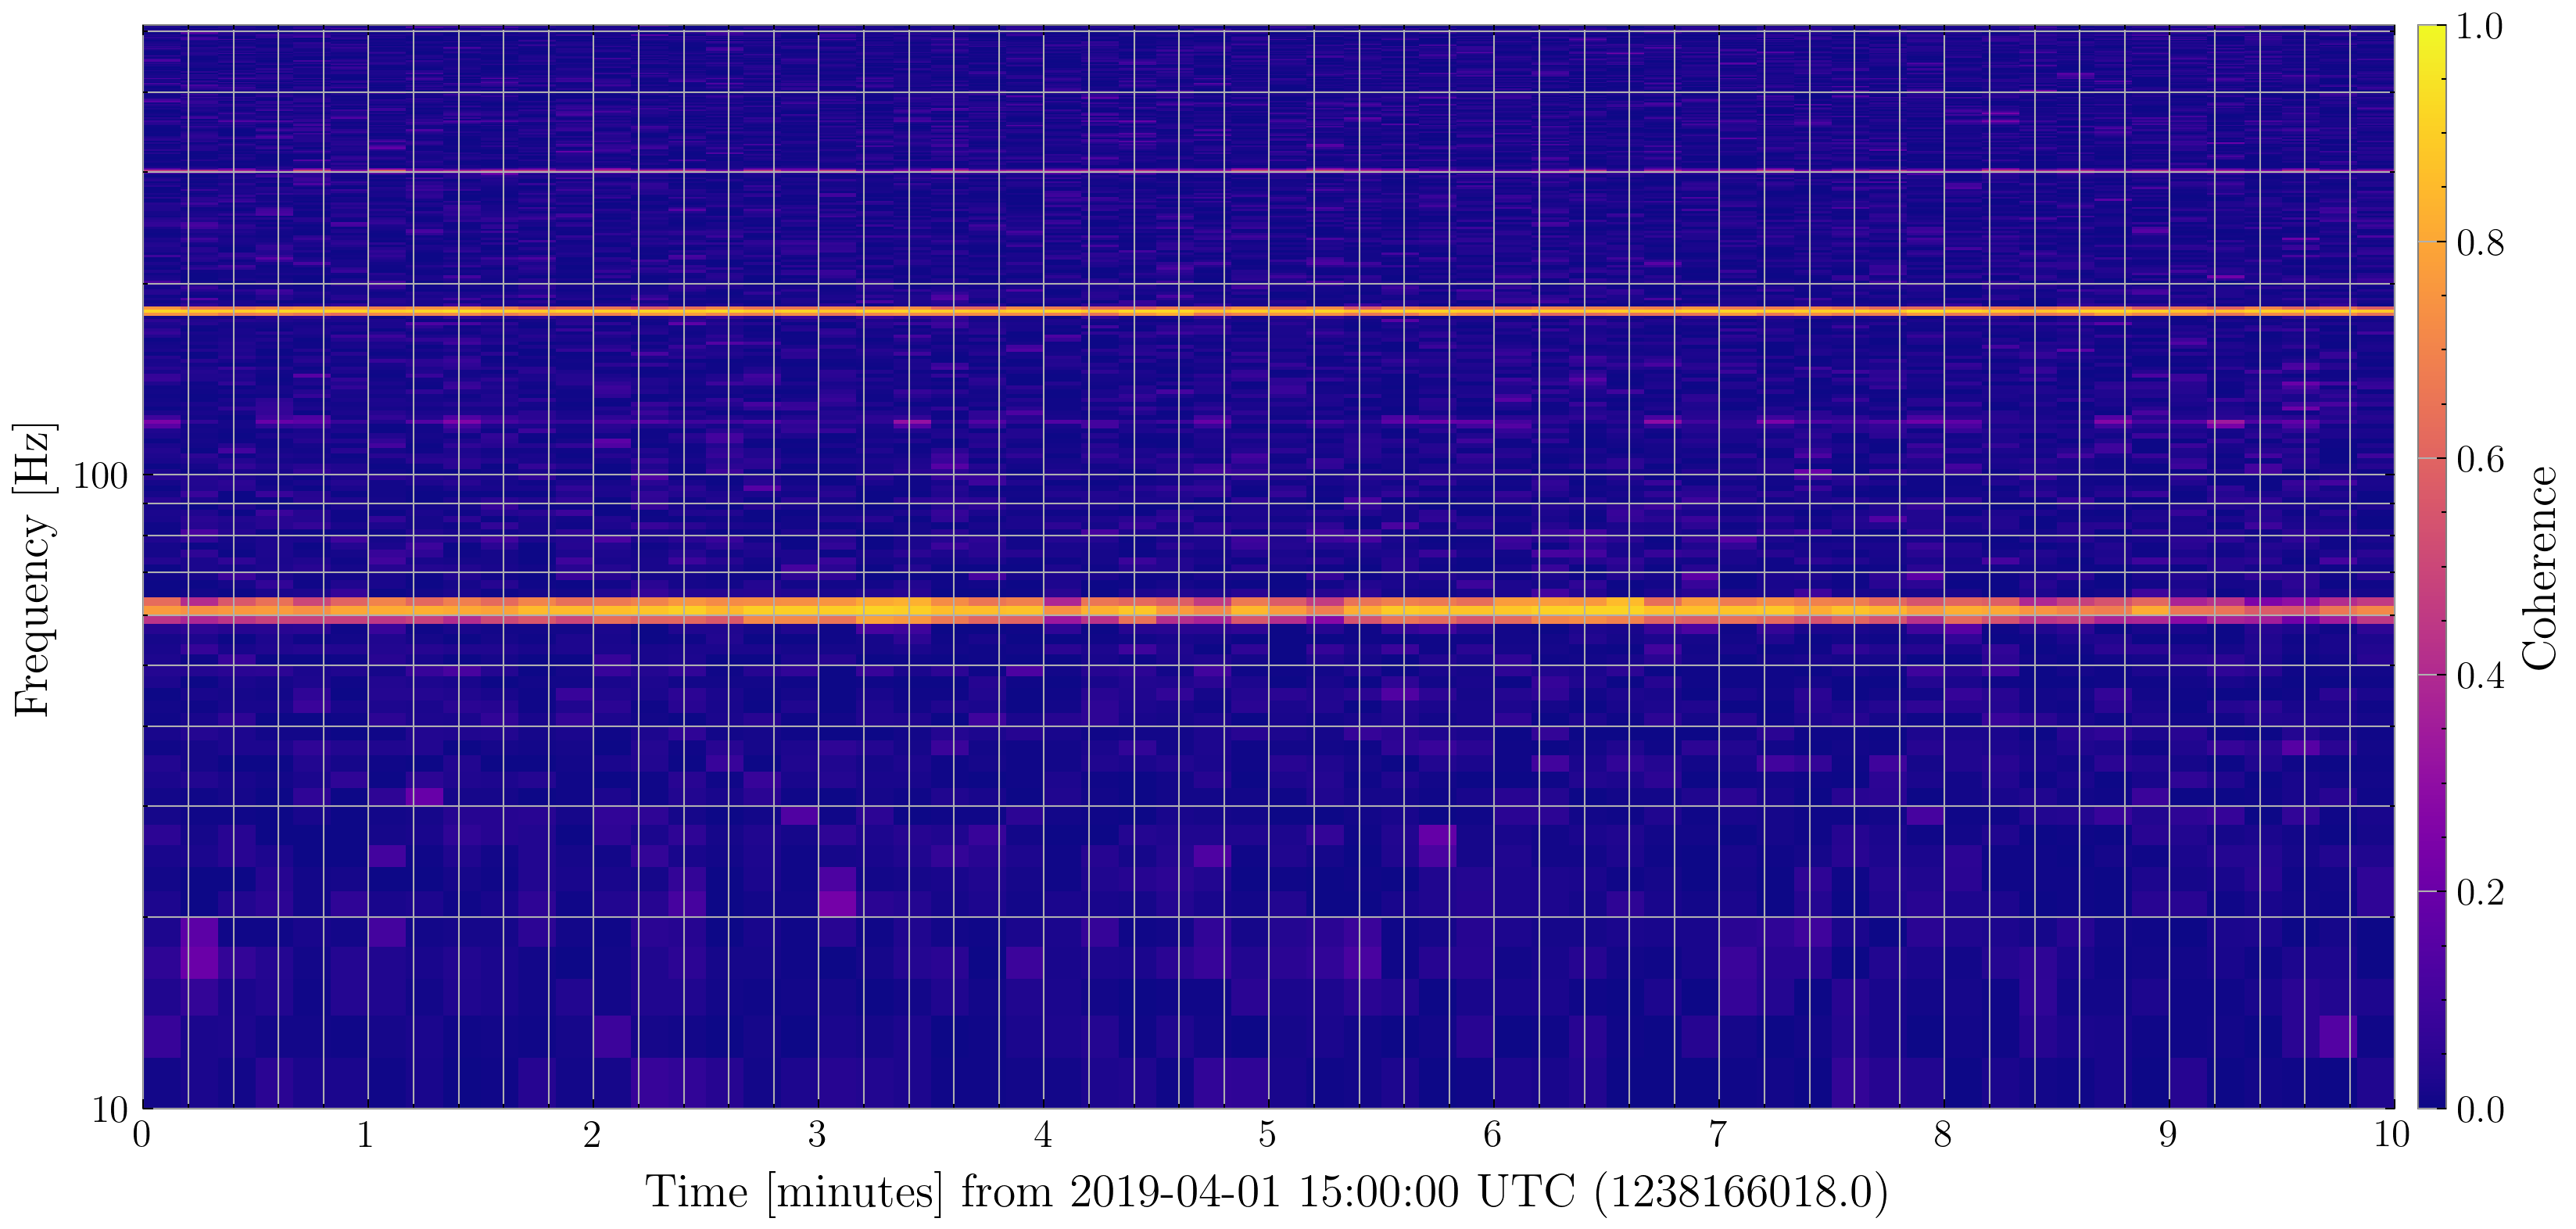
\includegraphics[width=\textwidth]{images/coherence_spectrogram}
%DIFDELCMD < 	%%%
\DIFdelendFL \DIFaddbeginFL 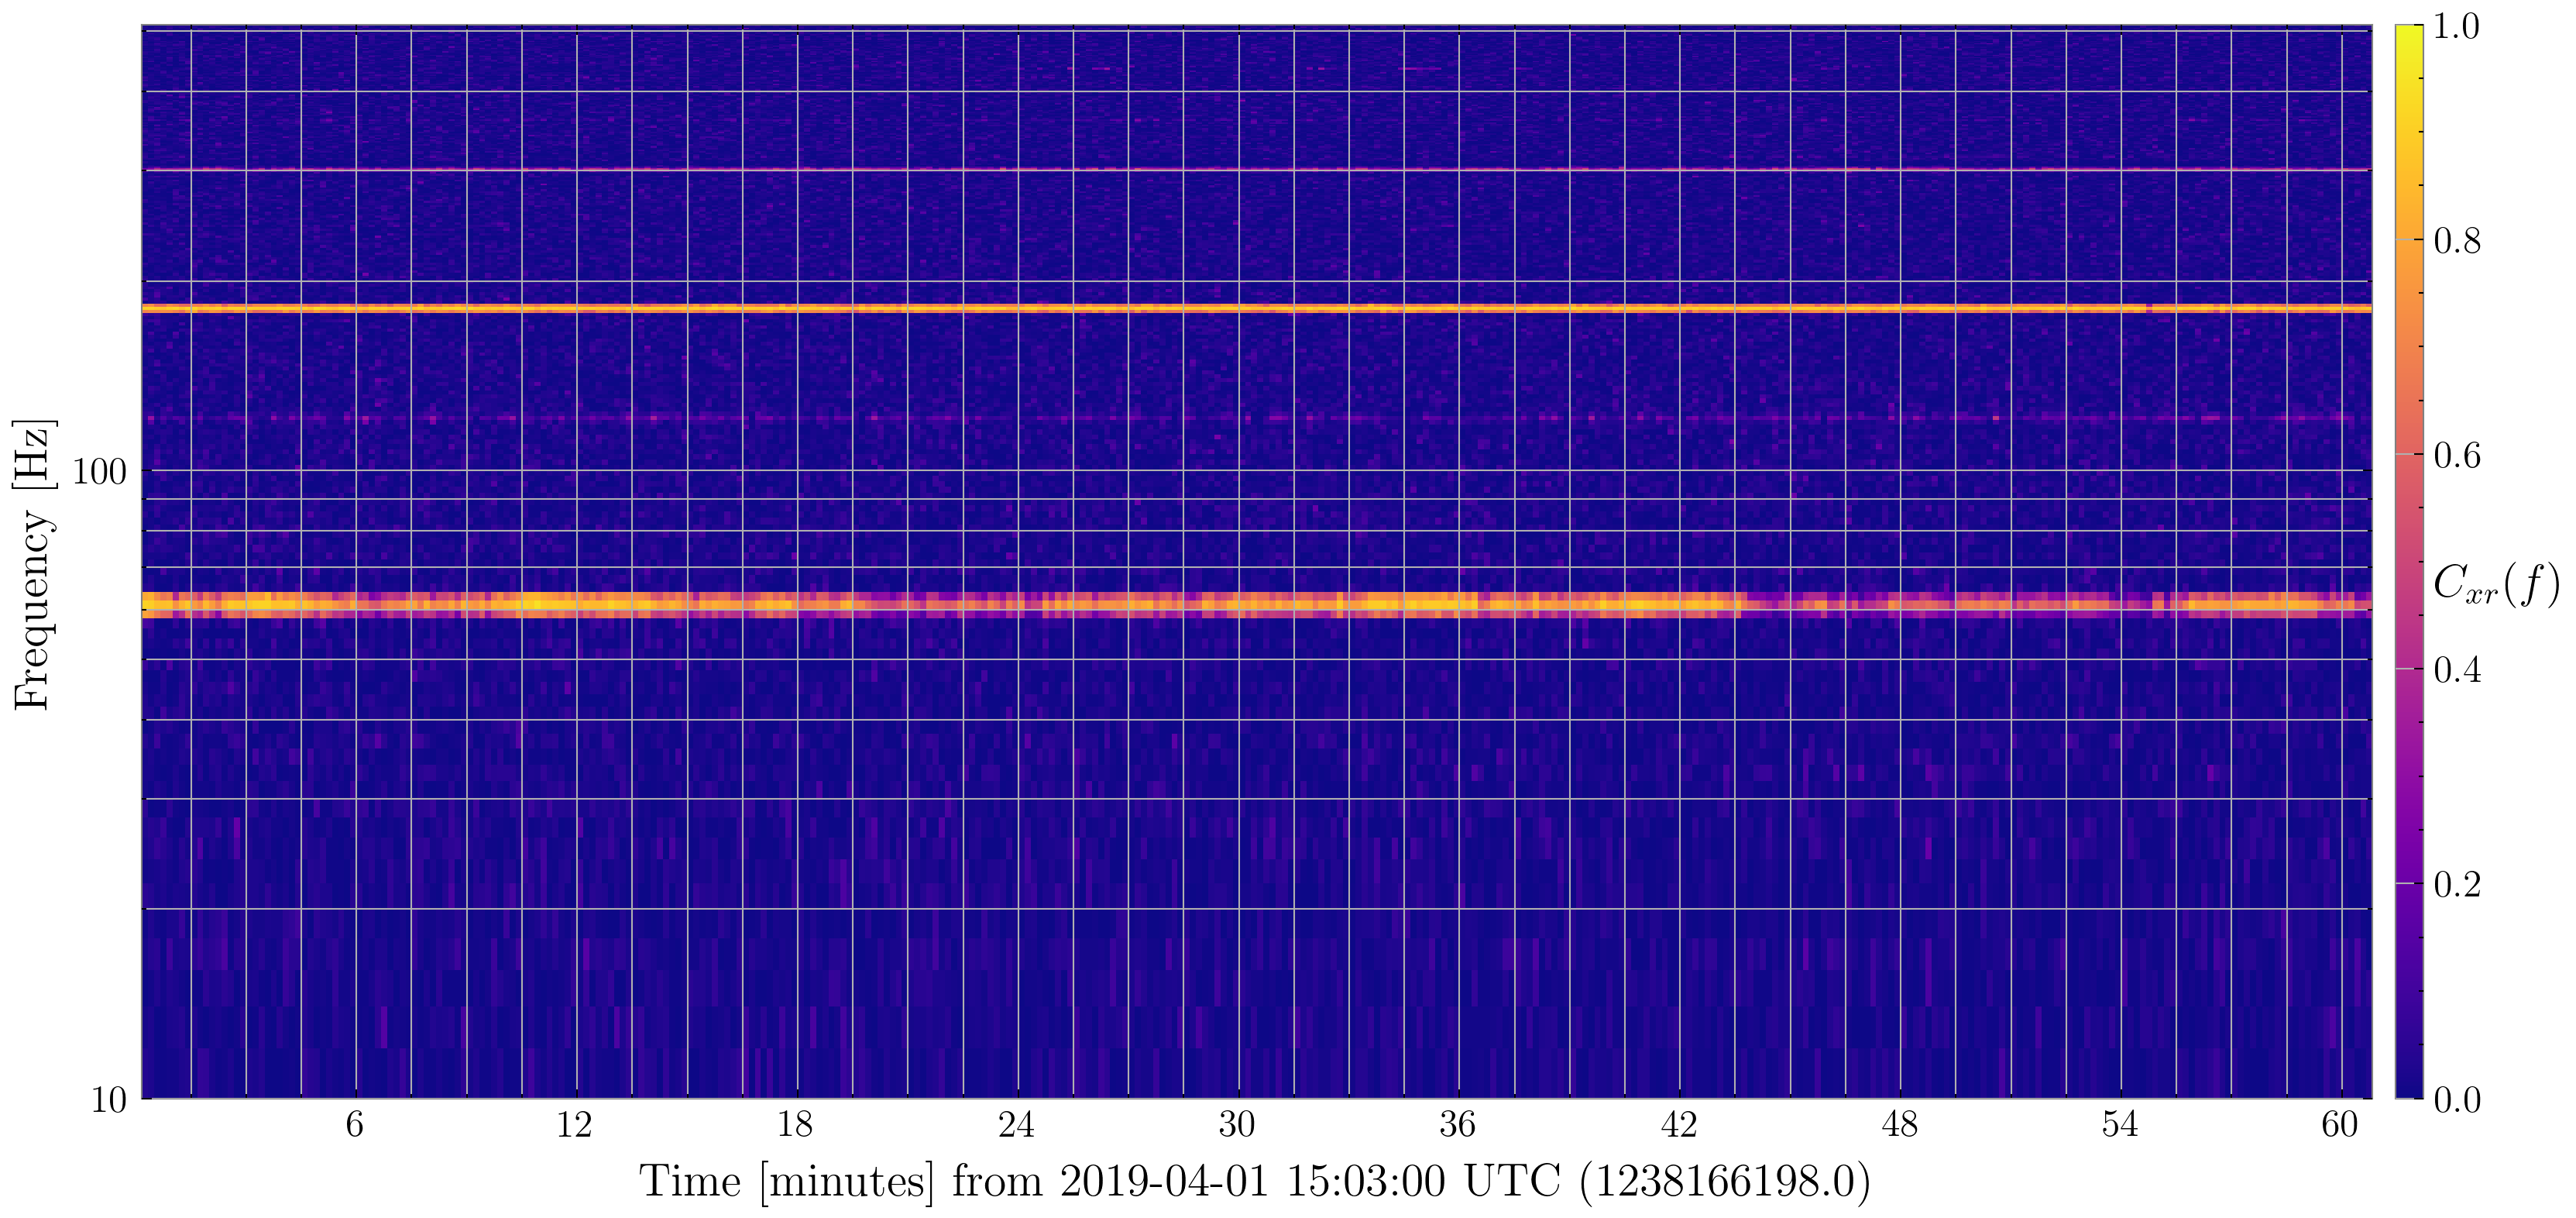
\includegraphics[width=\textwidth]{images/coherence_spectrogram_canonical}
	\DIFaddendFL \end{center}
	\caption{\label{correlation_1}
		Coherence spectrogram between the strain channel \StrainChanName  \DIFaddbeginFL \DIFaddFL{\, }\DIFaddendFL and the PEM channel \PEMChanName  	\DIFdelbeginFL \DIFdelFL{over }\DIFdelendFL \DIFaddbeginFL \DIFaddFL{\, covering }\DIFaddendFL a \DIFdelbeginFL \DIFdelFL{10 minute }\DIFdelendFL \DIFaddbeginFL \DIFaddFL{1 hour }\DIFaddendFL period of O3 data. \DIFaddbeginFL \DIFaddFL{The $x$-axis is the time in minutes from the start of O3a, separated into 10s bins. The $y$-axis is the frequency in Hz. The pixel colour denotes the coherence $C_{xy}$, Equation \eqref{eq:coherence}, in that time-frequency bin. }\DIFaddendFL A strong coherence is observed at \DIFdelbeginFL \DIFdelFL{60Hz }\DIFdelendFL \DIFaddbeginFL \DIFaddFL{60 Hz }\DIFaddendFL due to the main power interference. Additional coherence \DIFaddbeginFL \DIFaddFL{features }\DIFaddendFL can also be observed at \DIFdelbeginFL \DIFdelFL{$\sim$ 200 Hz }\DIFdelendFL \DIFaddbeginFL \DIFaddFL{0.2 kHz }\DIFaddendFL and \DIFdelbeginFL \DIFdelFL{300 Hz }\DIFdelendFL \DIFaddbeginFL \DIFaddFL{0.3 kHz }\DIFaddendFL due to instrumental lines of a different provenance c.f. \DIFdelbeginFL \DIFdelFL{Fig }\DIFdelendFL \DIFaddbeginFL \DIFaddFL{Figure }\DIFaddendFL \ref{fig:strainSensitivity}.}
\end{figure*}



\section{\DIFdelbegin \DIFdel{Adaptive Noise Cancellation}\DIFdelend \DIFaddbegin \DIFadd{ANC scheme}\DIFaddend }\label{sec:method}


Adaptive \DIFdelbegin \DIFdel{Noise Cancellation }\DIFdelend \DIFaddbegin \DIFadd{noise cancellation }\DIFaddend (ANC) is a method for recovering an estimate of an underlying signal \DIFdelbegin \DIFdel{which has been }\DIFdelend corrupted or obscured by some additive noise \DIFdelbegin \DIFdel{interference }\DIFdelend \cite{Widrow1451965}. In contrast to other common optimal filtering methods (e.g. Wiener, Kalman) ANC requires no \DIFdelbegin \DIFdel{a-priori }\DIFdelend \DIFaddbegin \textit{\DIFadd{a priori}} \DIFaddend knowledge of either the signal or the noise. Instead, ANC makes use of a reference input which is correlated in some unknown way \DIFdelbegin \DIFdel{to }\DIFdelend \DIFaddbegin \DIFadd{with }\DIFaddend the noise in the primary signal. \DIFdelbegin \DIFdel{This reference can then be }\DIFdelend \DIFaddbegin \DIFadd{The reference is }\DIFaddend filtered and subtracted from the primary data \DIFdelbegin \DIFdel{series }\DIFdelend so as to recover the underlying signal. For our purposes, the primary timeseries is the gravitational-wave strain channel\DIFaddbegin \DIFadd{, }\DIFaddend $x(t)$\DIFdelbegin \DIFdel{(Equation \eqref{eq:data}) }\DIFdelend \DIFaddbegin \DIFadd{, Equation \eqref{eq:data}, }\DIFaddend and the reference is a PEM recording \DIFdelbegin \DIFdel{voltage data from the power grid }\DIFdelend \DIFaddbegin \DIFadd{a mains voltage, }\DIFaddend $r(t)$\DIFdelbegin \DIFdel{(Equation \eqref{eq:voltage})}\DIFdelend \DIFaddbegin \DIFadd{, Equation \eqref{eq:voltage}}\DIFaddend . The objective of ANC is \DIFdelbegin \DIFdel{then }\DIFdelend to remove the clutter $c(t)$ \DIFdelbegin \DIFdel{of }\DIFdelend \DIFaddbegin \DIFadd{in }\DIFaddend Equation \eqref{eq:data} with the aid of $r(t)$ whilst leaving $h(t)$ i.e. the signal of interest, intact. \DIFdelbegin \DIFdel{We now describe the ANC implementation used in this work. }\DIFdelend \newline 

\DIFdelbegin \DIFdel{The reference  $r(t)$ is used to construct }\DIFdelend \DIFaddbegin \subsection{\DIFadd{Filter}}

\DIFadd{The first step in implementing ANC is to convert $r(t)$ into }\DIFaddend an estimate of the clutter, $\hat{c}(t)$. The clutter estimate \DIFdelbegin \DIFdel{can then be }\DIFdelend \DIFaddbegin \DIFadd{is }\DIFaddend subtracted from the primary signal in the time domain, defining a residual
\DIFdelbegin \DIFdel{$e(t)$:
}\DIFdelend \begin{eqnarray}
	e(t) = x(t) - \hat{c}(t) \ .\label{eq:error_estimate}
\end{eqnarray}
\DIFdelbegin \DIFdel{As }\DIFdelend \DIFaddbegin \DIFadd{In the limit }\DIFaddend $\hat{c}(t) \to c(t)$, \DIFaddbegin \DIFadd{one obtains	}\DIFaddend $e(t) \to h(t) + n(t)$ and \DIFdelbegin \DIFdel{we recover }\DIFdelend \DIFaddbegin \DIFadd{recovers }\DIFaddend a noise cancelled timeseries. The clutter estimate is modelled by a finite duration impulse response (FIR) filter\DIFdelbegin \DIFdel{:
}\DIFdelend \DIFaddbegin \DIFadd{,
}\DIFaddend \begin{eqnarray}
	\hat{c}_k = \mathbf{w}^{\intercal}\mathbf{u}_k \ . \label{clutter_estimate}
\end{eqnarray}
\DIFdelbegin \DIFdel{where $\hat{c}_k$ }\DIFdelend \DIFaddbegin \DIFadd{In Equation \eqref{clutter_estimate}, ${\hat c}_k = {\hat c}(t_{n_k})$ }\DIFaddend is the clutter estimate at \DIFdelbegin \DIFdel{a discrete timestep $k$ (i.e. $\hat{c}_k = \hat{c}(t_{n_k})$)}\DIFdelend \DIFaddbegin \DIFadd{the $n_k$-th time step }\DIFaddend , $\mathbf{u}_k$ is the tap-input vector composed of $M$ running samples of the reference signal arranged backwards in time\DIFdelbegin \DIFdel{:
 }\DIFdelend \DIFaddbegin \DIFadd{,
 }\DIFaddend \begin{eqnarray}
 	\mathbf{u}_k &= [r_k, r_{k-1}, \dots, r_{k-M+1}] \ ,
 \end{eqnarray}
and $\mathbf{w}$ is the tap-weight vector\DIFdelbegin \DIFdel{:
 }\DIFdelend \DIFaddbegin \DIFadd{,
 }\DIFaddend \begin{eqnarray}
	\mathbf{w} = [w_1, w_{2}, \dots, w_{M}] \ .
\end{eqnarray}
\DIFdelbegin \DIFdel{We want }\DIFdelend \DIFaddbegin 

\DIFadd{The goal of ANC is }\DIFaddend to determine the optimal tap weights $\mathbf{w}_{\rm opt}$, \DIFdelbegin \DIFdel{those which }\DIFdelend \DIFaddbegin \DIFadd{that }\DIFaddend minimise the mean square error cost function\DIFdelbegin \DIFdel{:
}\DIFdelend \DIFaddbegin \DIFadd{,
}\DIFaddend \begin{eqnarray}
	\mathbf{w}_{\rm opt} = \arg \min \sum\DIFdelbegin \DIFdel{_{t=t_1}^{t=t_{N}} }\DIFdelend \DIFaddbegin \DIFadd{_{k=1}^{K} \lambda^{K-k-1} }\DIFaddend |e\DIFdelbegin \DIFdel{(t)}\DIFdelend \DIFaddbegin \DIFadd{_k}\DIFaddend |^2 \ \DIFdelbegin \DIFdel{.
}\DIFdelend \DIFaddbegin \DIFadd{, }\label{eq:minim}
\DIFaddend \end{eqnarray}
\DIFdelbegin \DIFdel{This minimization problem }\DIFdelend \DIFaddbegin \DIFadd{where $0 \leq \lambda \leq 1$ is a ``forgetting factor" which gives exponentially less weight to older samples and can be freely chosen. The choice of $\lambda$ in this paper is discussed in Section \ref{sec:ARLS}. The minimization problem described by Equation \eqref{eq:minim} }\DIFaddend can be solved \DIFdelbegin \DIFdel{by way of an adaptive recursive least squares (ARLS ) method which we now describe }\DIFdelend \DIFaddbegin \DIFadd{in many ways. Here we implement an ARLS algorithm. The algorithm is outlined }\DIFaddend in Section \ref{sec:ARLS}

\subsection{\DIFdelbegin \DIFdel{Adaptive Recursive Least Squares Method}\DIFdelend \DIFaddbegin \DIFadd{ARLS algorithm}\DIFaddend }
\label{sec:ARLS}
\DIFdelbegin \DIFdel{We now outline the ARLS method to compute the optimal tap weights and estimate the noise-subtracted signal . 
}\DIFdelend \DIFaddbegin 

\DIFadd{As its name implies, the ARLS algorithm is adaptive, in the sense that the weights $\mathbf{w}$ are continually updated based on new data. It is also recursive, in the sense that $\mathbf{w}$ are updated iteratively as new data arrives, rather than reprocessing all previous data. Abbreviated pseudocode is presented below for the sake of reproducibility and the reader's convenience. The reader is referred to standard signal processing textbooks, e.g. \mbox{%DIFAUXCMD
\cite{HaykinAdaptiveFT:2002} }\hskip0pt%DIFAUXCMD
for more information. }\newline 

\DIFadd{ARLS proceeds as follows:
}

\DIFaddend \begin{enumerate}
	\item Initialise the tap weights $\mathbf{w} = \mathbf{0}$\DIFdelbegin \DIFdel{and }\DIFdelend \DIFaddbegin \DIFadd{. Initialise }\DIFaddend a covariance matrix \DIFdelbegin \DIFdel{$\mathbf{P}= \delta^{-1} \mathbf{I}$, }\DIFdelend \DIFaddbegin \DIFadd{${\bf P} = \langle {\bf w} {\bf w}^{\rm T} \rangle = \delta^{-1} {\bf I}$ of rank $M$ }\DIFaddend for regularisation parameter $0 < \delta \ll 1$  and \DIFaddbegin \DIFadd{an $M \times M$ }\DIFaddend identity matrix $\mathbf{I}$ \DIFdelbegin \DIFdel{of rank $M$}\DIFdelend \DIFaddbegin \DIFadd{where the superscript $T$ symbolises transposition}\DIFaddend .
	\item For \DIFdelbegin \DIFdel{$k=1, \dots, K$:
	}%DIFDELCMD < 

%DIFDELCMD < 	%%%
\DIFdelend \DIFaddbegin \DIFadd{$1 \leq k \leq K$:
	}\DIFaddend \begin{enumerate}
		\item Estimate the clutter $\hat{c}_k$ \DIFdelbegin \DIFdel{by Equation \ref{clutter_estimate}
		}\DIFdelend \DIFaddbegin \DIFadd{from Equation \eqref{clutter_estimate}
		}\DIFaddend \item Calculate the residual $e_k$ \DIFdelbegin \DIFdel{by Equation \ref{eq:error_estimate}
		}\DIFdelend \DIFaddbegin \DIFadd{from Equation \eqref{eq:error_estimate}
		}\DIFaddend \item Calculate the gain vector
		\begin{eqnarray}
			\mathbf{g}_k = \frac{\mathbf{P} \mathbf{u}_k}{\lambda + \mathbf{u}_k^{\intercal}\mathbf{P} \mathbf{u}_k}
		\end{eqnarray}
	\item Update the tap weights
			\begin{eqnarray}
		\mathbf{w}\DIFdelbegin \DIFdel{\mathrel{+}}\DIFdelend \DIFaddbegin \DIFadd{_k }\DIFaddend = \DIFaddbegin \DIFadd{\mathbf{w}_{k-1} +  }\DIFaddend e_k \mathbf{g}\DIFaddbegin \DIFadd{_k 
	}\DIFaddend \end{eqnarray}
	\item Update the covariance matrix
\begin{eqnarray}
	\mathbf{P}\DIFdelbegin \DIFdel{\mathrel{+}}\DIFdelend \DIFaddbegin \DIFadd{_k }\DIFaddend =  \DIFaddbegin \DIFadd{\mathbf{P}_{k-1}  }\DIFaddend \lambda^{-1}  \DIFdelbegin \DIFdel{\mathbf{P} }\DIFdelend - \mathbf{g}\DIFdelbegin \DIFdel{\lambda^{-1} \mathbf{P} }\DIFdelend \DIFaddbegin \DIFadd{_k }\DIFaddend \mathbf{u}_k^{\intercal}  \DIFaddbegin \DIFadd{\lambda^{-1} \mathbf{P}_{k-1} 
}\DIFaddend \end{eqnarray}

	\end{enumerate}

\end{enumerate}
The \DIFdelbegin \DIFdel{algorithm }\DIFdelend \DIFaddbegin \DIFadd{pseudocode }\DIFaddend is also illustrated in Figure \ref{fig:arlsBlock} via a block diagram. \DIFaddbegin \DIFadd{At time $t$ the filter receives the reference signal $r(t)$ and produces an estimate of the clutter $\hat{c}(t)$, given the current tap weights $\mathbf{w}$. By comparing $\hat{c}(t)$ with the strain data $x(t)$ a residual is calculated $e(t)$. The residual is then used in conjunction with $r(t)$ to update the weights and the algorithm continues iteratively. }\DIFaddend \newline 

\DIFdelbegin \DIFdel{ARLS has two }\DIFdelend %DIF > https://citeseerx.ist.psu.edu/viewdoc/download;jsessionid=597B4CA0A9E3A810EF9E49A466A02ADC?doi=10.1.1.4.2748&rep=rep1&type=pdf for groing wndow
\DIFaddbegin \DIFadd{ARLS has three }\DIFaddend free parameters: the order parameter $M$\DIFdelbegin \DIFdel{and the ``forgetting factor " }\DIFdelend \DIFaddbegin \DIFadd{, the forgetting factor }\DIFaddend $\lambda$, \DIFdelbegin \DIFdel{which is chosen so as to give exponentially less weight to older samples. The choice }\DIFdelend \DIFaddbegin \DIFadd{and the regularisation parameter $\delta$. Larger values }\DIFaddend of $M$ \DIFdelbegin \DIFdel{influences the latency of the FIR filter, }\DIFdelend \DIFaddbegin \DIFadd{corresponds to an increased model complexity. Whilst this generally increases the accuracy of the resulting estimates, it also increases }\DIFaddend the computational overhead and \DIFdelbegin \DIFdel{the filter accuracy}\DIFdelend \DIFaddbegin \DIFadd{hence the latency between receiving the input data and updating the weights}\DIFaddend . In Sec.~\ref{sec:results} we trial a selection of $M$ values for synthetic GW data. \DIFdelbegin \DIFdel{The forgetting factor$\lambda$ ranges between 0 and 1,  with }\DIFdelend \DIFaddbegin \DIFadd{Regarding the forgetting factor,  }\DIFaddend $\lambda=1$ \DIFdelbegin \DIFdel{corresponding }\DIFdelend \DIFaddbegin \DIFadd{corresponds }\DIFaddend to infinite memory, causing the filter becomes \DIFdelbegin \DIFdel{an ordinary least squares method}\DIFdelend \DIFaddbegin \DIFadd{a "growing window" RLS \mbox{%DIFAUXCMD
\citep{10.5555/547203,10.5555/560138}}\hskip0pt%DIFAUXCMD
}\DIFaddend . In this work we use $\lambda=0.9999$. \DIFaddbegin \DIFadd{Different values of $\lambda$ are investigated in Section \ref{sec:roc2}. The regularisation parameter $\delta$ must be ``suitably chosen" \mbox{%DIFAUXCMD
\citep{ljung1999system,1989system}}\hskip0pt%DIFAUXCMD
. A large $\delta$ leads to rapid convergence of the ARLS algorithm, but with correspondingly larger variance in the parameter estimates before convergence. Conversely, a smaller $\delta$ leads to slower convergence and smaller variance in the parameter estimates. General guidelines for choosing $\delta$ are not readily available. Instead $\delta$ is typically empirically selected for the particular problem. In this work we found $\delta = 100$ to be a reasonable choice, since we have a large uncertainty in our initial estimate of the weights. }\DIFaddend We refer the reader to Chapter 9 of Ref.~\cite{HaykinAdaptiveFT:2002} for a full review of adaptive least squares estimation in the context of linear filtering. 
\begin{figure}
	\begin{center}
		\DIFdelbeginFL %DIFDELCMD < 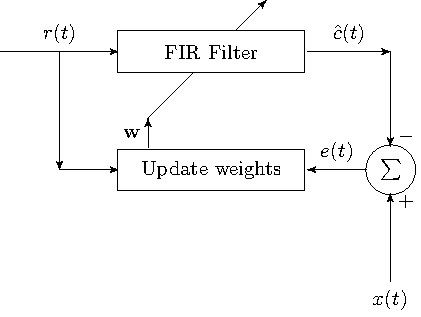
\includegraphics[width=\columnwidth]{images/FIR_block.pdf}
%DIFDELCMD < 	%%%
\DIFdelendFL \DIFaddbeginFL 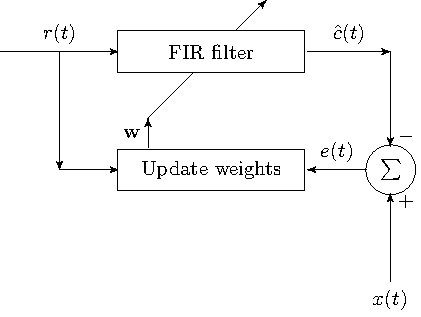
\includegraphics[width=\columnwidth]{images/fir_block_2.pdf}
	\DIFaddendFL \end{center}
	\caption{Block diagram of the \DIFdelbeginFL \DIFdelFL{adaptive recursive least squares }\DIFdelendFL \DIFaddbeginFL \DIFaddFL{ARLS }\DIFaddendFL method described in Section \ref{sec:ARLS}. The reference signal $r(t)$ is passed to an FIR filter to construct an estimate of the \DIFdelbeginFL \DIFdelFL{signal }\DIFdelendFL clutter\DIFdelbeginFL \DIFdelFL{$\hat{c}(t)$}\DIFdelendFL . Subtracting \DIFdelbeginFL \DIFdelFL{the clutter estimate }\DIFdelendFL \DIFaddbeginFL \DIFaddFL{$\hat{c}(t)$ }\DIFaddendFL from the primary signal $x(t)$ provides a residual $e(t)$ which \DIFdelbeginFL \DIFdelFL{can then be used }\DIFdelendFL \DIFaddbeginFL \DIFaddFL{controls the process }\DIFaddendFL to update \DIFaddbeginFL \DIFaddFL{to update }\DIFaddendFL the weights $\mathbf{w}$ of the FIR filter\DIFdelbeginFL \DIFdelFL{and the }\DIFdelendFL \DIFaddbeginFL \DIFaddFL{. The }\DIFaddendFL method proceeds iteratively. \DIFaddbeginFL \DIFaddFL{The diagonal line across the FIR filter block denotes that the parameters of the block (i.e. $\mathbf{w}$) are being updated, but are not part of the signal processed by the block.}\DIFaddendFL }
	\label{fig:arlsBlock}
\end{figure}

\section{\DIFdelbegin \DIFdel{HMM }\DIFdelend Validation tests \DIFaddbegin \DIFadd{with an HMM}\DIFaddend } \label{sec:results}
We \DIFdelbegin \DIFdel{want to }\DIFdelend test the ANC \DIFdelbegin \DIFdel{method described in the preceding section by trying }\DIFdelend \DIFaddbegin \DIFadd{scheme in Section \ref{sec:method} by combining it with a HMM }\DIFaddend to search for a \DIFdelbegin \DIFdel{continuous wave signal which has an initial frequency$f_{\rm GW}(t=0) = 60 $Hz, coincident with the instrumental linefrom the mains power grid. We search for the CW signal using a HMM scheme based on the Viterbi algorithm \mbox{%DIFAUXCMD
\cite{Viterbi1,viterbi2}}\hskip0pt%DIFAUXCMD
.  Specifically, we use the method }\DIFdelend \DIFaddbegin \DIFadd{CW signal with randomly wandering frequency, which overlaps the mains power line. Many other validation tests are possible, of course, and no individual test represents the final word on the efficacy of the scheme. Nonetheless, HMM-based searches are a key element of the data analysis program of the LVK Collaboration, generating a substantial corpus of published results \mbox{%DIFAUXCMD
\citep{LIGOMarkov17,LIGOMarkov19,PhysRevD.99.084042,2018PhRvD..97d3013S,LIGOMarkov22,2023PhRvD.107f4062V}}\hskip0pt%DIFAUXCMD
. In the context of this paper, validations tests involving a HMM are especially powerful, because they present the ANC scheme with an additional challenge: to subtract the mains power line well enough to reveal an underlying CW signal, which is itself ``noisy'' (in the sense that its frequency wanders) rather than monochromatic. That is, the ANC-HMM combination is tasked to not only remove the stochastic 60-Hz interference but also distinguish it from the process noise in the CW signal's frequency. If the ANC succeeds in this complicated task, one may be confident that it also succeeds in the easier task of subtracting the mains power line to reveal an underlying CW signal whose frequency is constant.  }\newline 

\DIFadd{In what follows, we employ the HMM scheme }\DIFaddend introduced by \citet{Suvorova2016PhRv}, which has been thoroughly tested through multiple LVK searches \cite{Piccinni2022,Riles2023,Wette2023}. We do not cover any details of the HMM scheme in this work and refer the reader to \citet{Suvorova2016PhRv} for further information. \DIFdelbegin \DIFdel{The GW signal is obscured in the data by the presence of the mains power instrumental line }\DIFdelend \DIFaddbegin \DIFadd{A synthetic CW signal $h(t)$, whose frequency executes an unbiased random walk, is injected into synthetic Gaussian noise $n(t)$ typical of the LIGO detectors. A simulated 60-Hz mains power line $c(t)$ is superposed, whose properties mimic the real system (see Section \ref{sec22})}\DIFaddend . The challenge is to \DIFdelbegin \DIFdel{try to recover the signal by first }\DIFdelend \DIFaddbegin \DIFadd{recover the $h(t)$ by }\DIFaddend passing the data $x(t)$ through the ANC filter \DIFdelbegin \DIFdel{before using the HMM tracker on this filtered dataset to try to recover the signal}\DIFdelend \DIFaddbegin \DIFadd{and feeding the output into the HMM tracker}\DIFaddend . In Section \ref{sec:creating_data} we describe how we create a synthetic \DIFdelbegin \DIFdel{dataset }\DIFdelend \DIFaddbegin \DIFadd{time series }\DIFaddend $x(t)$. In Section \ref{sec:representative_example} we \DIFdelbegin \DIFdel{introduce }\DIFdelend \DIFaddbegin \DIFadd{present }\DIFaddend a representative example \DIFdelbegin \DIFdel{, illustrating the frequency tracking }\DIFdelend \DIFaddbegin \DIFadd{and compare the HMM's ability to detect and track $h(t)$ }\DIFaddend before and after \DIFdelbegin \DIFdel{ANC. In Section \ref{sec:roc1} we explore the performance of the ANC filter in response to different characteristics of the interference signal, e.g. variations in the central frequency $f_{\rm ac}$ relative to the initial GW frequency. In Section \ref{sec:roc2} we investigate the performance of the filter in response to different filter settings; the order of the filter $M$ (i.e. the number of taps) and the number of reference channel inputs.
}\DIFdelend \DIFaddbegin \DIFadd{applying ANC. 
}\DIFaddend 

\DIFdelbegin \subsection{\DIFdel{Creating simulated data}} %DIFAUXCMD
\addtocounter{subsection}{-1}%DIFAUXCMD
%DIFDELCMD < \label{sec:creating_data}
%DIFDELCMD < %%%
\DIFdel{Throughout this paper we work with some }\DIFdelend \DIFaddbegin \subsection{\DIFadd{Synthetic data}} \label{sec:creating_data}
\DIFadd{In the tests that follow, we work with }\DIFaddend representative synthetic data, \DIFdelbegin \DIFdel{$x(t)$}\DIFdelend \DIFaddbegin \DIFadd{generated under controlled conditions}\DIFaddend , rather than directly with the LIGO data\DIFdelbegin \DIFdel{itself}\DIFdelend . We can \DIFdelbegin \DIFdel{construct }\DIFdelend \DIFaddbegin \DIFadd{generate }\DIFaddend synthetic data for \DIFdelbegin \DIFdel{each of the constituent parts }\DIFdelend \DIFaddbegin \DIFadd{the constituents }\DIFaddend of Equation \eqref{eq:data} - \DIFdelbegin \DIFdel{the GW signal of interest, the Gaussian noise and the noise clutter via the formulation described }\DIFdelend \DIFaddbegin \DIFadd{namely $h(t)$, $c(t)$, and $n(t)$, by applying the recipe }\DIFaddend in Section \ref{sec21} as follows. \newline 

\DIFdelbegin \DIFdel{The GW frequency evolves in general due to  the intrinsic evolution of the due to the intrinsic evolution of the source. For this paper  }\DIFdelend \DIFaddbegin \DIFadd{Starting with $h(t)$ }\DIFaddend we assume that the source is isolated (i.e. \DIFdelbegin \DIFdel{it is }\DIFdelend not in a binary) and that the GW \DIFdelbegin \DIFdel{is monochromatic (i.e. all temporal derivatives of the frequency are zero}\DIFdelend \DIFaddbegin \DIFadd{signal is quasimonochromatic (i.e. the frequency varies slowly over many wave cycles if at all}\DIFaddend ). We also \DIFdelbegin \DIFdel{consider the GW source to be at a constant location with respect to the observer and neglect all contributions due to e.g. }\DIFdelend \DIFaddbegin \DIFadd{place the source at a fixed sky position and neglect for simplicity }\DIFaddend the rotation and revolution of the Earth. \DIFaddbegin \DIFadd{The latter corrections are included readily in searches with real data through the maximum likelihood ${\cal F}$-statistic \mbox{%DIFAUXCMD
\citep{Jaranowski1998}}\hskip0pt%DIFAUXCMD
. }\DIFaddend Under these assumptions the GW model reduces to 
\begin{equation}
	h(t) = h\DIFdelbegin \DIFdel{\sin(2\pi \phi_{\rm GW}(t)) }\DIFdelend \DIFaddbegin \DIFadd{_0\sin[2\pi \phi_{\rm gw}(t)] }\DIFaddend \ , 
\end{equation}
where \DIFdelbegin \DIFdel{$h$ }\DIFdelend \DIFaddbegin \DIFadd{$h_0$ }\DIFaddend is the constant \DIFdelbegin \DIFdel{GW amplitudeand $\phi(t)$ }\DIFdelend \DIFaddbegin \DIFadd{amplitude, $\phi_{\rm gw}(t)$ }\DIFaddend a random phase\DIFdelbegin \DIFdel{variable which is the integral of the underlying,
piecewise linear GW frequency $f_{\rm gw}$ i.e.
}\DIFdelend \DIFaddbegin \DIFadd{,
}\DIFaddend \begin{equation}
	\phi\DIFdelbegin \DIFdel{_{\rm GW}}\DIFdelend \DIFaddbegin \DIFadd{_{\rm gw}}\DIFaddend (t) = \int_{0}^{t} \DIFaddbegin \DIFadd{ds \, }\DIFaddend f_{\rm gw}(s)  \DIFdelbegin \DIFdel{ds }\DIFdelend \ \DIFdelbegin \DIFdel{.
}\DIFdelend \DIFaddbegin \DIFadd{,
}\DIFaddend \end{equation}
\DIFdelbegin \DIFdel{The GW frequency at discrete timestep $m$ within the sampling interval $\Delta t$ is labelled as $f_{\rm gw}^{(m)}$ and evolves according to
}\DIFdelend \DIFaddbegin \DIFadd{and the GW frequency $f_{\rm gw}(t)$ evolves stochastically and piecewise linearly from one time step to the next according to
}\DIFaddend \begin{eqnarray}
	f_{\rm gw}\DIFdelbegin \DIFdel{^{(m+1)} }\DIFdelend \DIFaddbegin \DIFadd{(t_{n+1}) }\DIFaddend = f_{\rm gw}\DIFdelbegin \DIFdel{^{(m)} + \delta_m \Delta }\DIFdelend \DIFaddbegin \DIFadd{(}\DIFaddend t\DIFdelbegin \DIFdel{\ ,
}\DIFdelend \DIFaddbegin \DIFadd{_n) + \epsilon_n 
}\DIFaddend \end{eqnarray}
\DIFdelbegin \DIFdel{with $\delta_m$ a zero mean Gaussian noise at timestep $m$}\DIFdelend \DIFaddbegin \DIFadd{where $\epsilon_n$ is a zero-mean Gaussian random variable}\DIFaddend , with variance $\sigma_f^2$ \DIFdelbegin \DIFdel{,
}\DIFdelend \DIFaddbegin \DIFadd{viz.
}\DIFaddend \begin{equation}
	\DIFdelbegin \DIFdel{\delta_m }\DIFdelend \DIFaddbegin \DIFadd{\epsilon_n }\DIFaddend = \mathcal{N}(0, \DIFaddbegin \DIFadd{\Delta t  \, }\DIFaddend \sigma_f^2) \DIFaddbegin \DIFadd{\ . }\DIFaddend \label{eq:gwfreqnoise}
\end{equation}
\DIFdelbegin \DIFdel{The }\DIFdelend \DIFaddbegin \DIFadd{Hence the }\DIFaddend synthetic GW signal $h(t)$ is \DIFdelbegin \DIFdel{then }\DIFdelend completely described by the parameters \DIFdelbegin \DIFdel{$h$ and $\sigma_f^2$, and the initial GW frequency }\DIFdelend \DIFaddbegin \DIFadd{$h_0$, $\sigma_f$, and }\DIFaddend $f_{\rm gw}(t=0)$ \newline 


The clutter and reference \DIFdelbegin \DIFdel{signal }\DIFdelend \DIFaddbegin \DIFadd{signals }\DIFaddend evolve according to Equations \eqref{eq:voltage} and \eqref{eq:vclutter} respectively. For this initial study we take the \DIFdelbegin \DIFdel{reference voltage to have a constant amplitude }\DIFdelend \DIFaddbegin \DIFadd{amplitudes }\DIFaddend $A_r(t) = a_r$ \DIFdelbegin \DIFdel{, the clutter to have a corresponding constant amplitude }\DIFdelend \DIFaddbegin \DIFadd{and }\DIFaddend $A_c(t) = a_c$ \DIFaddbegin \DIFadd{to be constants. Similarly, $P(t) = P=$ constant}\DIFaddend . \DIFdelbegin \DIFdel{We also assume that the modulation in the reference voltage about $f_{\rm ac}$ has a constantamplitude $\Delta f_{\rm ac}$ with a constant period $P(t) = P$. Throughout this work we take $\Delta f_{\rm ac} = 1/2\pi$ Hz }\footnote{%DIFDELCMD < \tiny %%%
\DIFdel{\textcolor{red}{TK: I have guessed that this is what is happening under the hood of the code, but need to verify with Sofia/Changrong.}}%DIFDELCMD < \normalsize%%%
}%DIFAUXCMD
\addtocounter{footnote}{-1}%DIFAUXCMD
\DIFdel{. We define the variable $\gamma = P^{-1}$ and explore different values for $\gamma$ }\DIFdelend \DIFaddbegin \DIFadd{Different values for $P$ are explored }\DIFaddend in Section \ref{sec:roc1}. Under these assumptions, Equations \eqref{eq:voltage} and \eqref{eq:vclutter} reduce to 
\begin{align}
 	r(t) =&a_r \cos \left[ 2 \pi f_{\rm ac} t +2 \pi \DIFaddbegin \DIFadd{\Delta f_{\rm ac} }\DIFaddend \cos\left(\DIFdelbegin \DIFdel{2 \pi \gamma t}\DIFdelend \DIFaddbegin \DIFadd{\frac{2 \pi t}{P}}\DIFaddend \right) + n_{\Theta} (t\DIFaddbegin \DIFadd{_n}\DIFaddend ) \right] \DIFdelbegin %DIFDELCMD < \\ %%%
\DIFdelend \nonumber \DIFaddbegin \\ 
 	\DIFaddend &+n_r(t\DIFaddbegin \DIFadd{_n}\DIFaddend ) \ ,
\end{align}
\DIFdelbegin \begin{eqnarray*}
	\DIFdel{c(t) = }&\DIFdel{a_c \cos \left[ 2 \pi f_{\rm ac} t' + 2 \pi \cos\left(2 \pi \gamma t' \right) + n_{\Theta} (t')\right] \ .
}\end{eqnarray*}%DIFAUXCMD
\DIFdelend \DIFaddbegin \begin{align}
	\DIFadd{c(t) = a_c \cos }&\DIFadd{\biggl \{ 2 \pi f_{\rm ac} (t_n - \tau_{\rm delay}) \nonumber }\\ 
	&\DIFadd{+ 2 \pi \Delta f_{\rm ac} \cos \biggl [ \frac{2 \pi (t_n - \tau_{\rm delay)}}{P} \biggr ] \nonumber }\\ 
	&\DIFadd{+ n_{\Theta} (t_n - \tau_{\rm delay}) \biggr \}
	\label{eq:clutterequation}
}\end{align}\DIFaddend 
The synthetic reference and clutter data are \DIFdelbegin \DIFdel{then completely }\DIFdelend \DIFaddbegin \DIFadd{fully }\DIFaddend described by the \DIFdelbegin \DIFdel{amplitude parameters $a_r,a_c$, the central frequency $f_{\rm ac}$, the timescale $\gamma$ and the noise covariances $\sigma^2_{\Theta}$, }\DIFdelend \DIFaddbegin \DIFadd{parameters $a_r,a_c,f_{\rm ac}, \Delta f_{\rm ac}, P,\sigma^2_{\Theta}$, }\DIFaddend $\sigma_r^2$. \DIFdelbegin \DIFdel{For convenience we reparametrise $f_{\rm ac}$ relative to the initial GW frequency at $t=0$, defining the new variable
}\begin{eqnarray*}
	\DIFdel{\Delta f = |f_{\rm ac} - f_{\rm gw}(t=0)|
}\end{eqnarray*}%DIFAUXCMD
\DIFdel{The 9 free parameters of the model }\DIFdelend \DIFaddbegin \newline 




\DIFadd{The 11 free parameters }\DIFaddend are summarised in Table \DIFdelbegin \DIFdel{\ref{tab:parameterdescription2}. We have 3 }\DIFdelend \DIFaddbegin \DIFadd{\ref{tab:parameterdescription1}, along with their chosen injected values. There are three }\DIFaddend amplitude parameters $h, a_r, a_c$\DIFdelbegin \DIFdel{for the GW, reference and clutter respectively, }\DIFdelend \DIFaddbegin \DIFadd{, }\DIFaddend with $h \ll a_c, a_r$. There are \DIFdelbegin \DIFdel{4 noise parameters $\sigma_n, \sigma_{\Theta}, \sigma_r, \sigma_f$ for the Gaussian noise $n(t)$, the voltage phase noise $n_{\Theta}(t)$, reference  signal measurement noise $n_r(t)$ and the GW frequency noise Equation \ref{eq:gwfreqnoise} respectively. Additionally we have the absolute difference between the central frequency and the initial GW frequency, $\Delta f$ and the timescale of the modulation in the central frequency,$\gamma$. }%DIFDELCMD < \newline 
%DIFDELCMD < 

%DIFDELCMD < %%%
\DIFdel{Throughout this work when creating synthetic data, }\DIFdelend \DIFaddbegin \DIFadd{four noise parameters $\sigma_n^2, \sigma_{\Theta}^2, \sigma_r^2$ and  $\sigma_f^2$. In this paper $\sigma_n^2$ and $\sigma_r^2$ have fixed, constant values, whilst different values for $\sigma_f^2$ and $\sigma_{\Theta}^2$ are investigated in Section \ref{sec:representative_example} and Section \ref{sec:roc1} respectively. There are three additional parameters that specify the modulation of the central frequency: $f_{\rm ac}$, $\Delta f_{\rm ac}$ and $P$. In this paper }\DIFaddend $f_{\rm ac}$ is fixed at 60 Hz. \DIFdelbegin \DIFdel{The terrestrial noise parameters, $\sigma_n^2$,$\sigma_r^2$,$\sigma_{\Theta}^2$ are also fixed. \textcolor{red}{TK: other summary text on choice of parameters for synthetic data to go here. Waiting on input from Sofia on which parameters were actually used for the data}
}%DIFDELCMD < \begin{table}[bp]
%DIFDELCMD < 	%%%
\DIFdelendFL \DIFaddbeginFL \DIFaddFL{Different values of $\Delta f_{\rm ac}$ and $P$ are investigated in Section \ref{sec:roc1}. Finally there is the initial G frequency, $f_{\rm gw}(t=0)$.
}

%\begin{table*}
%	\DIFaddendFL 
%
%	\DIFdelbeginFL %DIFDELCMD < \begin{tabular}{llc}
%%DIFDELCMD < 		%%%
%\DIFdelendFL \DIFaddbeginFL \begin{tabular}{llcc}
%		\DIFaddendFL \hline 
%
%		 \DIFdelbeginFL \DIFdelFL{Parameter }\DIFdelendFL \DIFaddbeginFL \multirow{2}{*}{Parameter} \DIFaddendFL & \DIFdelbeginFL \DIFdelFL{Physical meaning }\DIFdelendFL \DIFaddbeginFL \multirow{2}{*}{Physical meaning}  \DIFaddendFL & \DIFdelbeginFL \DIFdelFL{Injected Value }\DIFdelendFL \DIFaddbeginFL \multicolumn{2}{c}{Injected Value} \DIFaddendFL \\
%		\DIFaddbeginFL \cline{3-4}
%			 &  &\DIFaddFL{Section \ref{sec:results} }& \DIFaddFL{Section \ref{sec:theroccurves}    }\\
%		\DIFaddendFL \hline
%		\DIFdelbeginFL \DIFdelFL{$h$  }\DIFdelendFL \DIFaddbeginFL \DIFaddFL{$h_0$  }\DIFaddendFL &    \DIFdelbeginFL \DIFdelFL{Strain }\DIFdelendFL \DIFaddbeginFL \DIFaddFL{GW strain }\DIFaddendFL amplitude & \DIFdelbeginFL \DIFdelFL{- }\DIFdelendFL \DIFaddbeginFL \DIFaddFL{0.025}& \DIFaddFL{0.022 }\DIFaddendFL \\ 
%		$a_r$ & \DIFdelbeginFL \DIFdelFL{Voltage amplitude }\DIFdelendFL \DIFaddbeginFL \DIFaddFL{Mains voltage amplitude at PEM }\DIFaddendFL & \DIFdelbeginFL \DIFdelFL{- }\DIFdelendFL \DIFaddbeginFL \DIFaddFL{$\mathcal{U}(10-0.01,10+0.01)$}& \DIFaddFL{$\mathcal{U}(10-0.01,10+0.01)$ }\DIFaddendFL \\
%		$a_c$ & \DIFdelbeginFL \DIFdelFL{Clutter }\DIFdelendFL \DIFaddbeginFL \DIFaddFL{Interference voltage }\DIFaddendFL amplitude &\DIFdelbeginFL \DIFdelFL{- }\DIFdelendFL \DIFaddbeginFL \DIFaddFL{$\mathcal{U}(1.2-0.001,1.2+0.001)$}& \DIFaddFL{$\mathcal{U}(1.2-0.001,1.2+0.001)$ }\DIFaddendFL \\
%		\DIFdelbeginFL %DIFDELCMD < 
%
%%DIFDELCMD < 		
%%DIFDELCMD < 		%%%
%\DIFdelendFL $\sigma_n^2$ & \DIFdelbeginFL \DIFdelFL{Gaussian noise covariance}\DIFdelendFL \DIFaddbeginFL \DIFaddFL{Strain channel measurement noise }\DIFaddendFL &\DIFdelbeginFL \DIFdelFL{- }\DIFdelendFL \DIFaddbeginFL \DIFaddFL{1}& \DIFaddFL{1 }\DIFaddendFL \\
%		$\sigma_r^2$  & \DIFdelbeginFL \DIFdelFL{Voltage }\DIFdelendFL \DIFaddbeginFL \DIFaddFL{PEM voltage }\DIFaddendFL measurement noise & \DIFdelbeginFL \DIFdelFL{-}\DIFdelendFL \DIFaddbeginFL \DIFaddFL{$10^{-4}$}&\DIFaddFL{$10^{-4}$ }\DIFaddendFL \\
%		$\sigma_{\Theta}^2$ & \DIFdelbeginFL \DIFdelFL{Voltage }\DIFdelendFL \DIFaddbeginFL \DIFaddFL{PEM voltage }\DIFaddendFL phase noise  & \DIFdelbeginFL \DIFdelFL{-}\DIFdelendFL \DIFaddbeginFL \DIFaddFL{$10^{-2}$}& \DIFaddFL{$\{ 10^{-3}, 10^{-2}, 10^{-1}\}$}\DIFaddendFL \\
%		$\sigma^2_f$ &  GW frequency noise & \DIFdelbeginFL \DIFdelFL{-}\DIFdelendFL \DIFaddbeginFL \DIFaddFL{$\{0.01,0.1\}$}& \DIFaddFL{0.0016}\DIFaddendFL \\
%		\DIFdelbeginFL %DIFDELCMD < 
%
%%DIFDELCMD < 		%%%
%\DIFdelFL{$\Delta f$ }\DIFdelendFL \DIFaddbeginFL \DIFaddFL{$f_{\rm gw}(t=0)$ }\DIFaddendFL &  \DIFdelbeginFL \DIFdelFL{Central frequency shift  }\DIFdelendFL \DIFaddbeginFL \DIFaddFL{Initial GW frequency  }\DIFaddendFL & \DIFdelbeginFL \DIFdelFL{-}\DIFdelendFL \DIFaddbeginFL \DIFaddFL{59.5 Hz}& \DIFaddFL{59.9 Hz}\DIFaddendFL \\
%		\DIFdelbeginFL \DIFdelFL{$\gamma$ }\DIFdelendFL \DIFaddbeginFL \DIFaddFL{$ f_{\rm ac}$ }&  \DIFaddFL{Central interference frequency }\DIFaddendFL & \DIFdelbeginFL \DIFdelFL{Modulation frequency }\DIFdelendFL \DIFaddbeginFL \DIFaddFL{60 Hz}\DIFaddendFL & \DIFdelbeginFL \DIFdelFL{- }\DIFdelendFL \DIFaddbeginFL \DIFaddFL{60 Hz}\DIFaddendFL \\ 
%		\DIFaddbeginFL \DIFaddFL{$\Delta f_{\rm ac}$ }&  \DIFaddFL{Amplitude of interference frequency modulation  }& \DIFaddFL{1 Hz}& \DIFaddFL{$\{0.5, 1.0, 1.5\}$ Hz}\\
%		\DIFaddFL{$P$ }& \DIFaddFL{Period of interference frequency modulation }& \DIFaddFL{$10^2$ s}& \DIFaddFL{$\{ 10^{1}, 10^2, 10^3\}$ s }\\
%		\DIFaddendFL \hline
%
%	\end{tabular} 
%
%	\caption{\DIFdelbeginFL \DIFdelFL{Summary of parameters }\DIFdelendFL \DIFaddbeginFL \DIFaddFL{Parameters, their physical meaning, and the injected values }\DIFaddendFL used to \DIFdelbeginFL \DIFdelFL{create }\DIFdelendFL \DIFaddbeginFL \DIFaddFL{generate }\DIFaddendFL synthetic data\DIFaddbeginFL \DIFaddFL{. The injected values are listed }\DIFaddendFL for \DIFdelbeginFL \DIFdelFL{testing }\DIFdelendFL \DIFaddbeginFL \DIFaddFL{validating }\DIFaddendFL the ANC \DIFdelbeginFL \DIFdelFL{method }\DIFdelendFL \DIFaddbeginFL \DIFaddFL{scheme }\DIFaddendFL in Section \ref{sec:results}, \DIFdelbeginFL \DIFdelFL{their physical meaning, }\DIFdelendFL and \DIFaddbeginFL \DIFaddFL{quantifying }\DIFaddendFL the \DIFaddbeginFL \DIFaddFL{performance of the scheme as a function of the properties of the mains power interference in Section  \ref{sec:theroccurves}. $a_r$ and $a_c$ are randomly drawn from separate uniform distributions. The braces notation (e.g. $\{0.01, 0.1\}$) indicates that multiple }\DIFaddendFL injected values \DIFdelbeginFL \DIFdelFL{used throughout this work}\DIFdelendFL \DIFaddbeginFL \DIFaddFL{have been trialled}\DIFaddendFL . \DIFaddbeginFL \DIFaddFL{The quoted injected values have been scaled such that $\sigma_n^2 = 1$.}\DIFaddendFL }
%	\DIFdelbeginFL %DIFDELCMD < \label{tab:parameterdescription2}
%%DIFDELCMD < \end{table}
%%DIFDELCMD < %%%
%\DIFdelend \DIFaddbegin \label{tab:parameterdescription1}
%\end{table*}
\DIFaddend 



\subsection{Representative \DIFdelbegin \DIFdel{example}\DIFdelend \DIFaddbegin \DIFadd{worked examples}\DIFaddend } \label{sec:representative_example}
\begin{figure}
	\begin{center}
		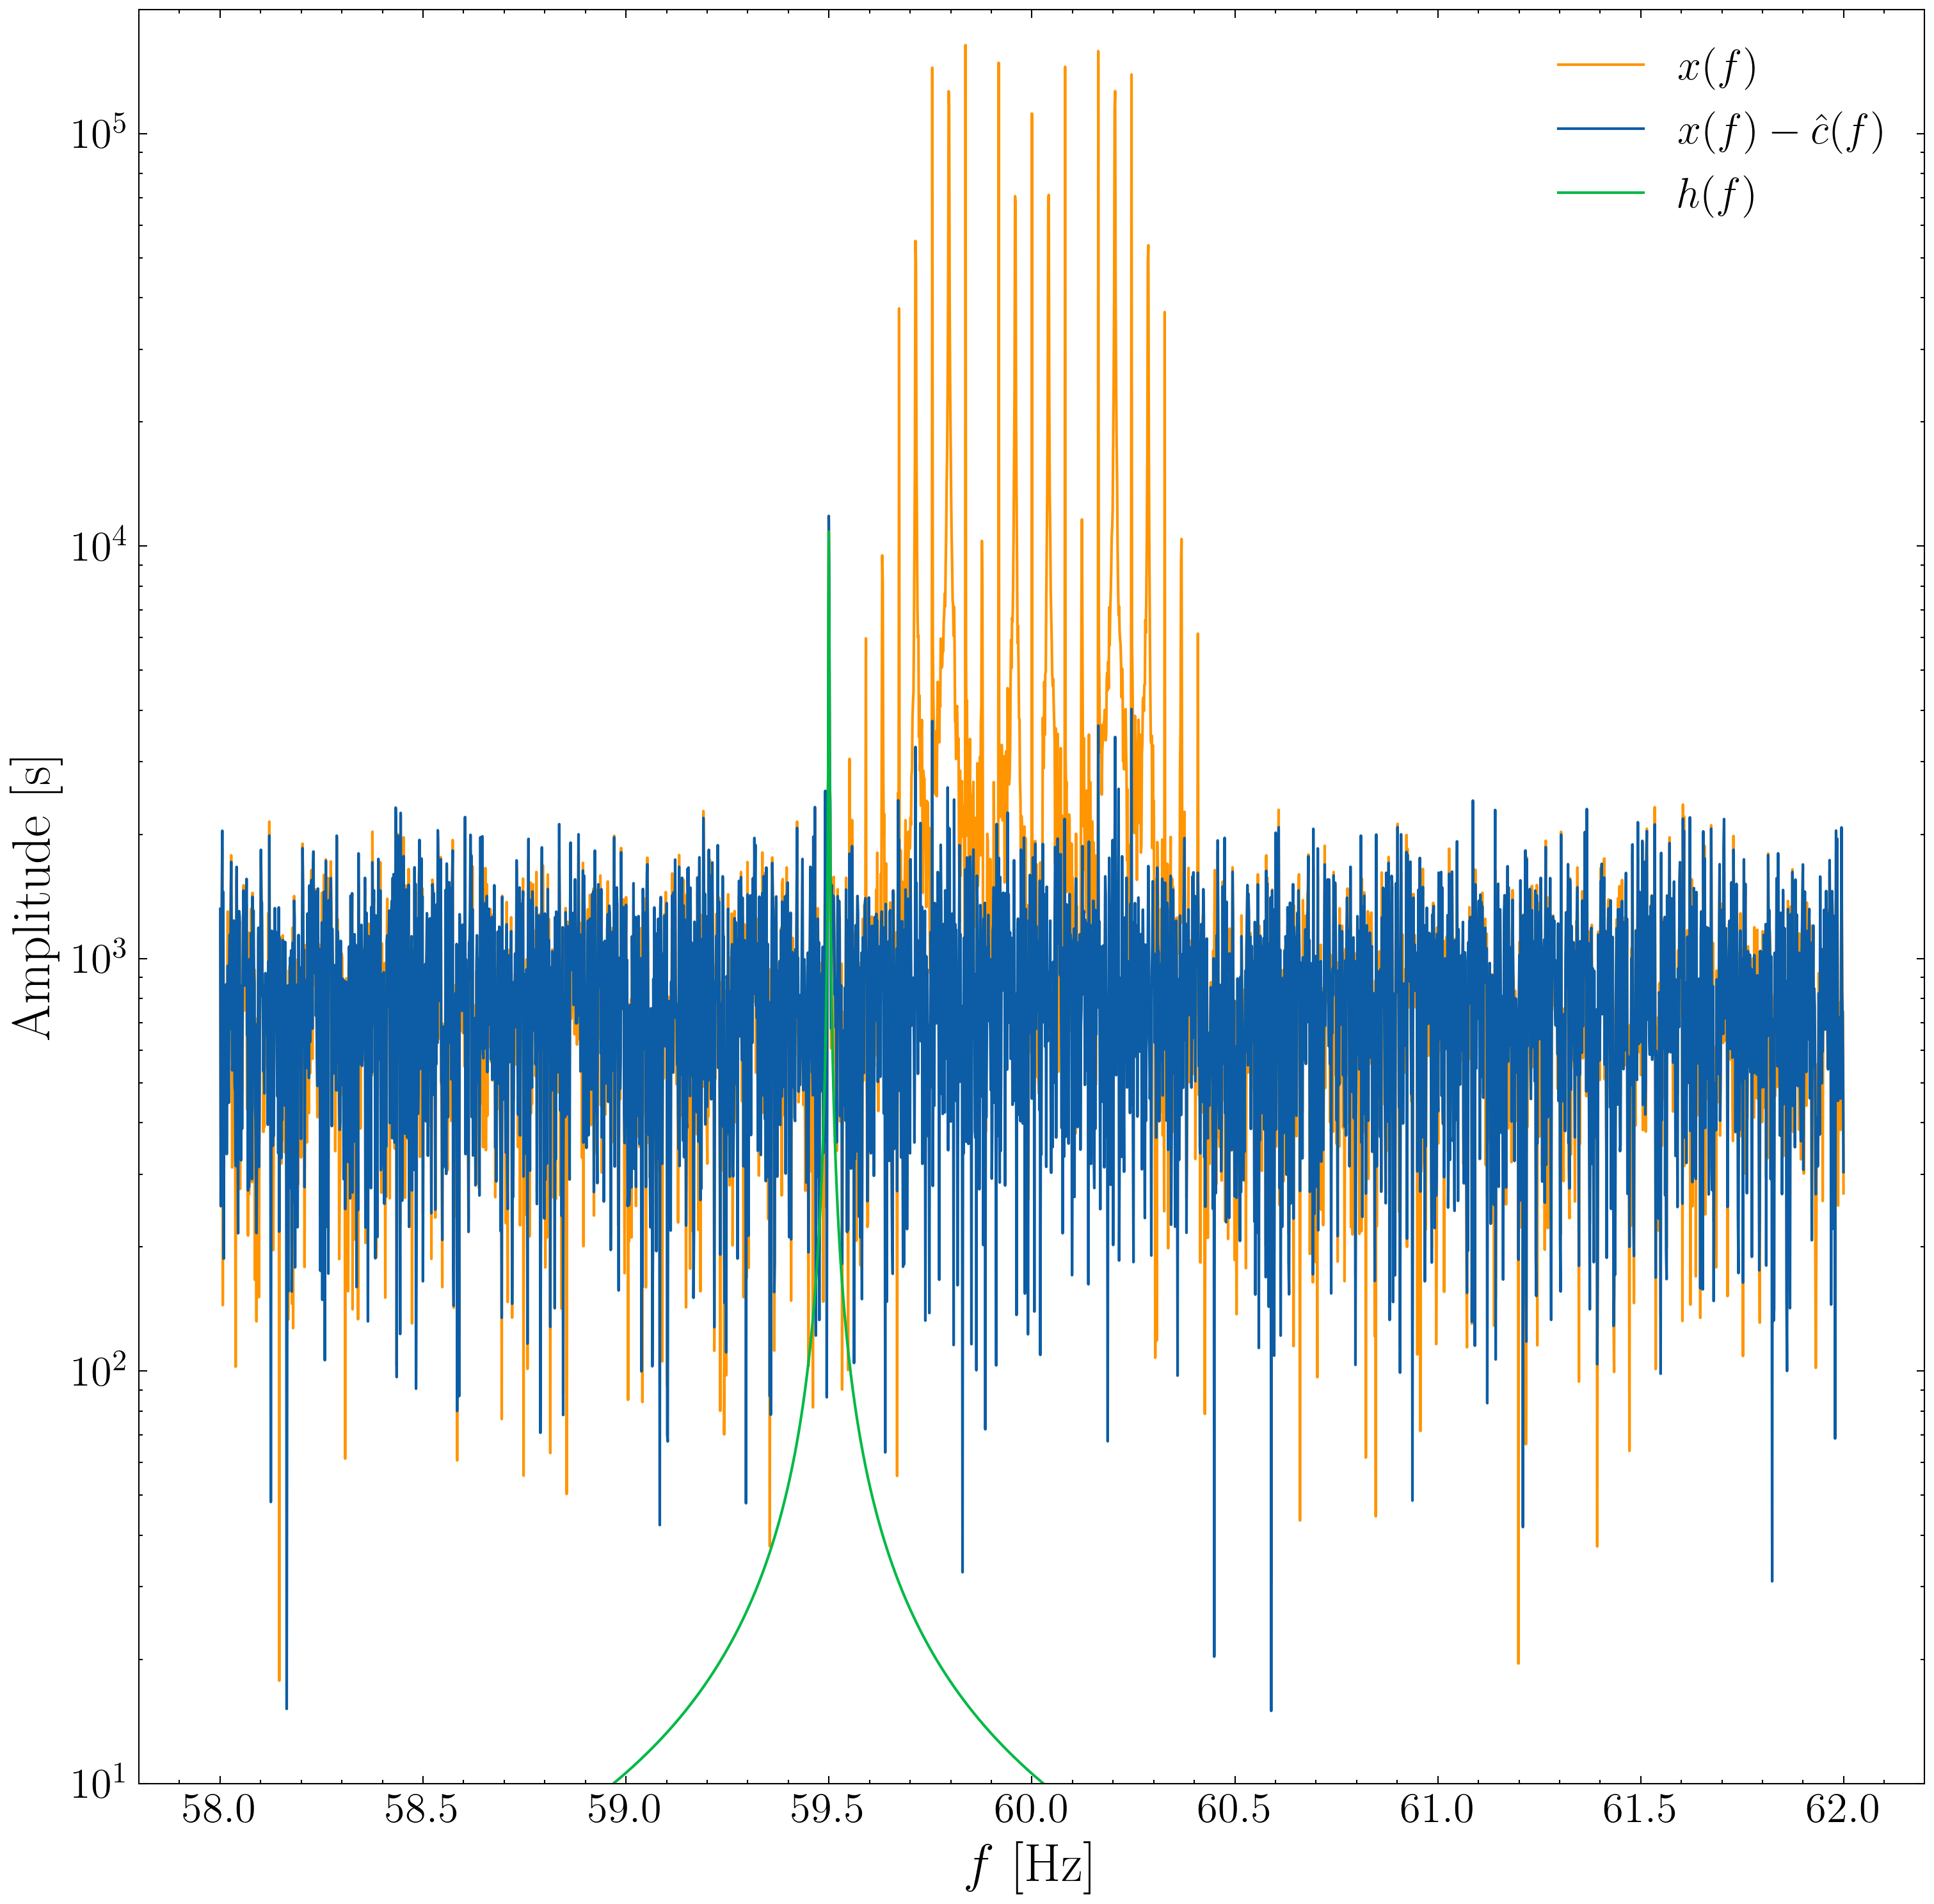
\includegraphics[width=\columnwidth]{images/spectrum.png}
	\end{center}
	\caption{\DIFaddbeginFL \DIFaddFL{Spectrum (i.e.\ modulus of the }\DIFaddendFL Fourier \DIFdelbeginFL \DIFdelFL{response }\DIFdelendFL \DIFaddbeginFL \DIFaddFL{transform) }\DIFaddendFL of the data $x(t)$ (orange \DIFaddbeginFL \DIFaddFL{curve}\DIFaddendFL ), \DIFdelbeginFL \DIFdelFL{the }\DIFdelendFL GW signal $h(t)$ (green \DIFaddbeginFL \DIFaddFL{curve}\DIFaddendFL ) and \DIFaddbeginFL \DIFaddFL{decluttered output of }\DIFaddendFL the ANC \DIFdelbeginFL \DIFdelFL{filtered data }\DIFdelendFL \DIFaddbeginFL \DIFaddFL{filter }\DIFaddendFL $x(t) - \hat{c}(t)$ (blue \DIFaddbeginFL \DIFaddFL{curve}\DIFaddendFL ) for a system with parameters described in Table \DIFdelbeginFL \DIFdelFL{\ref{tab:parameterdescription2}}\DIFdelendFL \DIFaddbeginFL \DIFaddFL{\ref{tab:parameterdescription1}}\DIFaddendFL . ANC \DIFdelbeginFL \DIFdelFL{filters out }\DIFdelendFL \DIFaddbeginFL \DIFaddFL{suppresses }\DIFaddendFL the \DIFdelbeginFL \DIFdelFL{excess }\DIFdelendFL \DIFaddbeginFL \DIFaddFL{orange spikes near $60 \, {\rm Hz}$, which corresponding to mains }\DIFaddendFL power \DIFdelbeginFL \DIFdelFL{that results from the }\DIFdelendFL interference\DIFdelbeginFL \DIFdelFL{signal about the central 60 Hz frequency}\DIFdelendFL \DIFaddbeginFL \DIFaddFL{, by $\approx 20\, {\rm dB}$}\DIFaddendFL .}
	\label{fig:spectrum}
\end{figure}
\begin{figure*}
	\begin{center}
			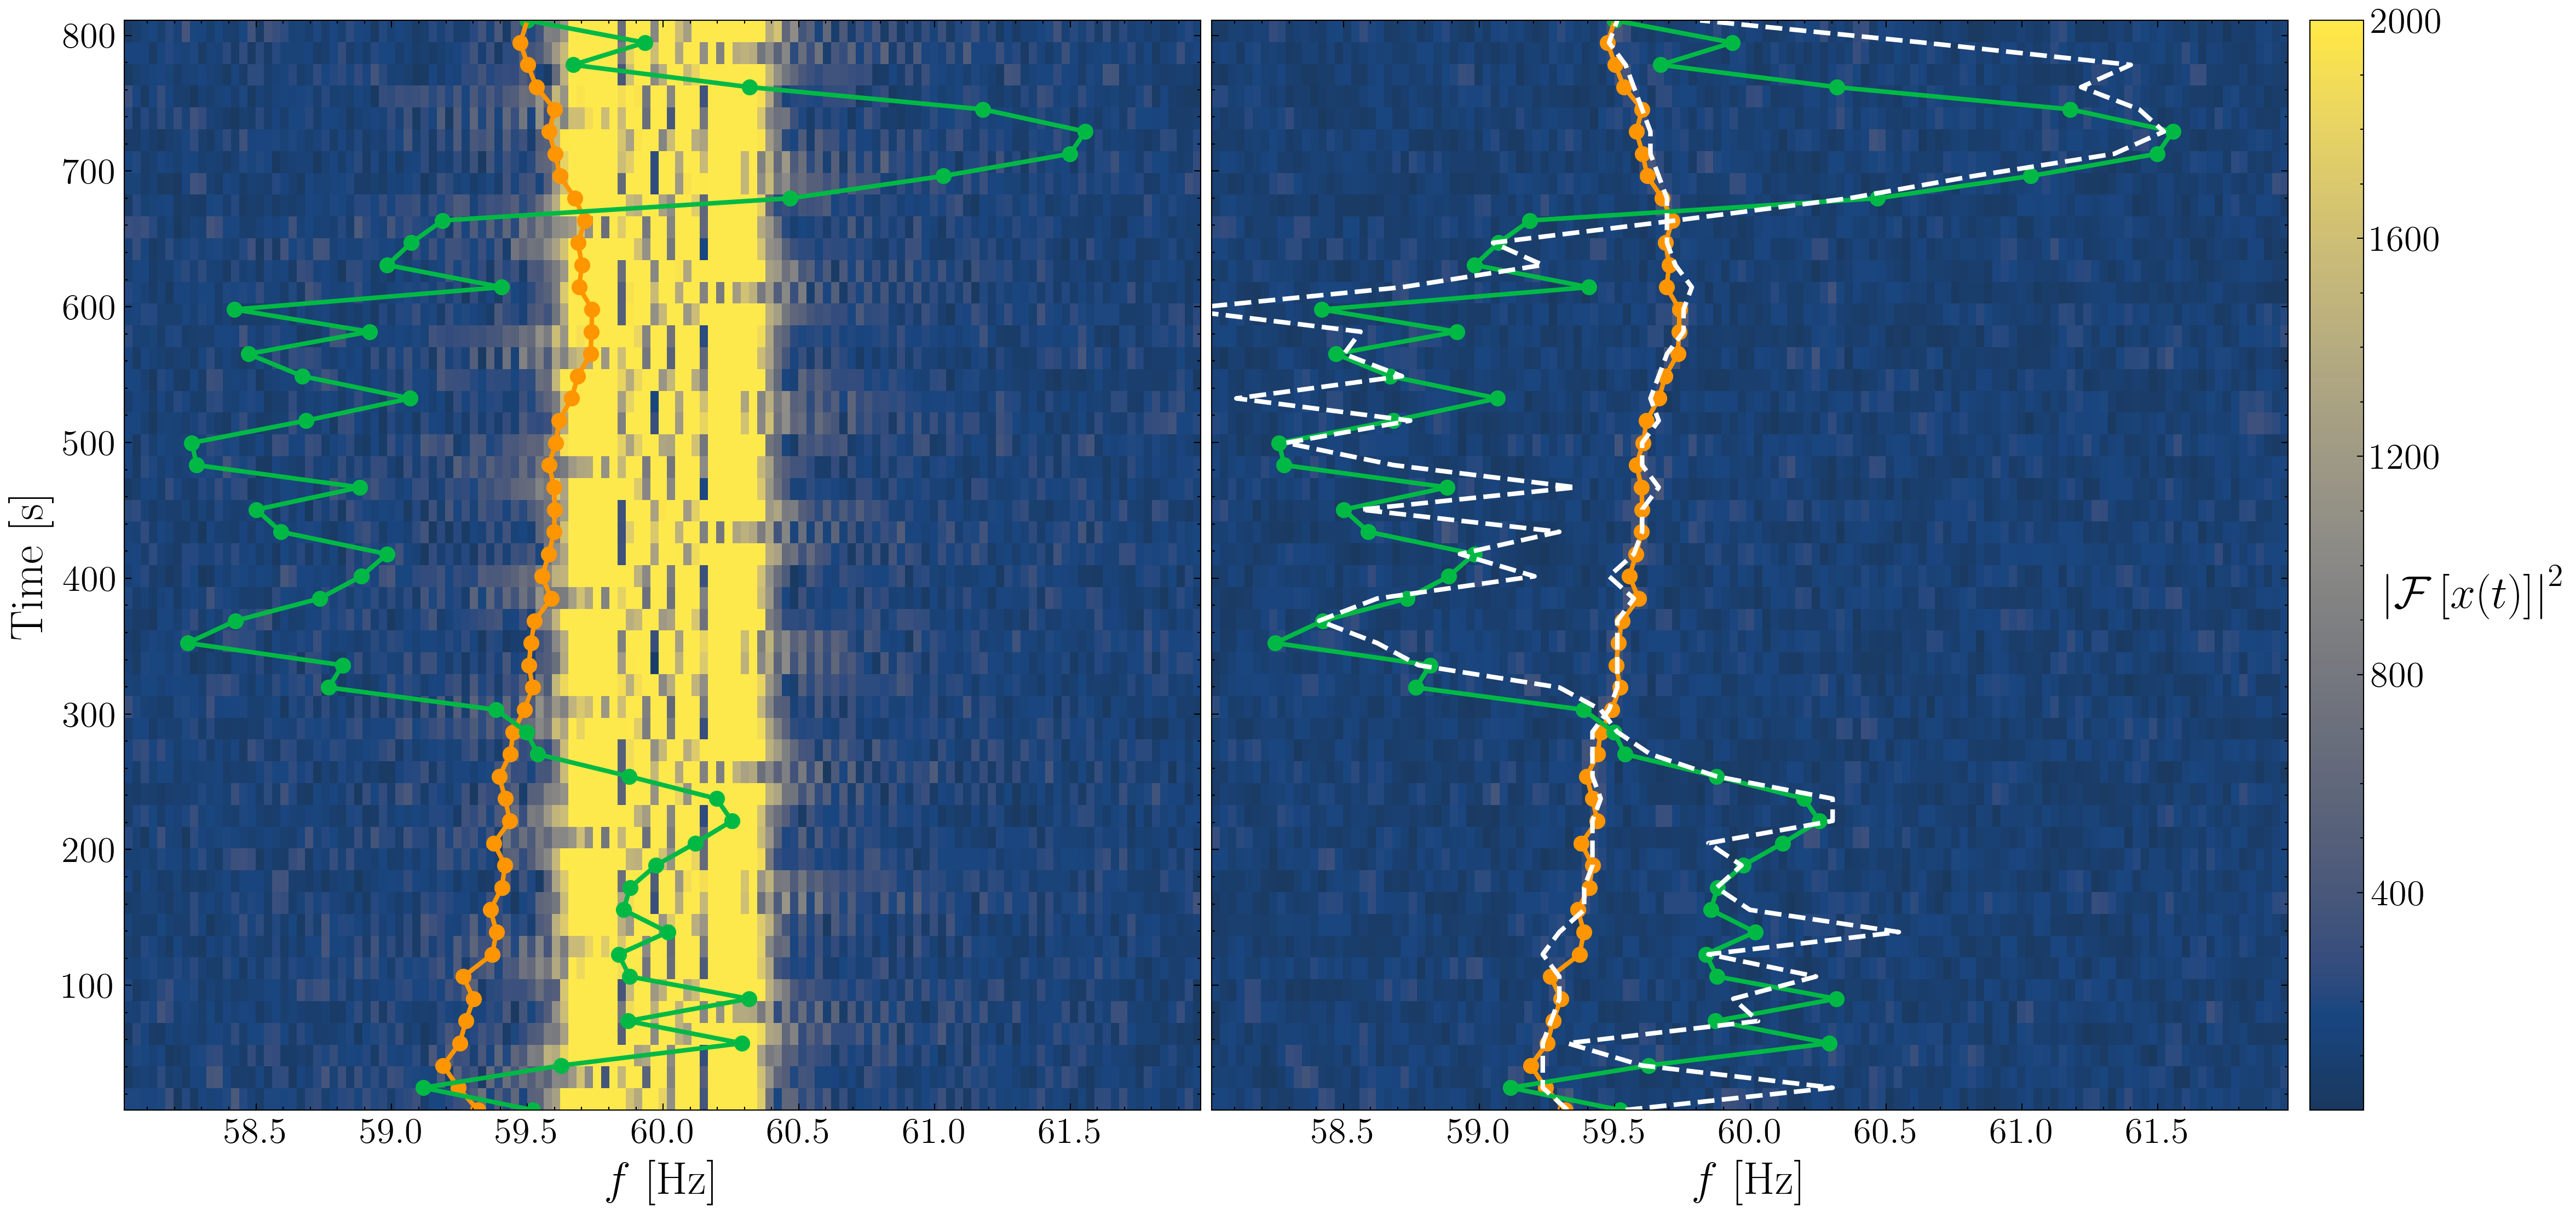
\includegraphics[width=\textwidth]{images/viterbi_tracking_canonical}
		\end{center}
	\caption{\label{frequency tracking before and after1}
			\DIFdelbeginFL \DIFdelFL{Fourier amplitude spectrogram and }\DIFdelendFL \DIFaddbeginFL \DIFaddFL{HMM }\DIFaddendFL tracking of \DIFdelbeginFL \DIFdelFL{the frequency evolution of }\DIFdelendFL a \DIFdelbeginFL \DIFdelFL{continuous GW }\DIFdelendFL \DIFaddbeginFL \DIFaddFL{CW signal }\DIFaddendFL with \DIFdelbeginFL \DIFdelFL{$h = 0.025$ and $\sigma_f^2 = \{0.01, 0.1\}$ Hz $s^{-1/2}$ }\DIFdelendFL \DIFaddbeginFL \DIFaddFL{spin wandering in the presence of $60 \, {\rm Hz}$ mains power interference before }\DIFaddendFL (\DIFdelbeginFL \DIFdelFL{orange }\DIFdelendFL \DIFaddbeginFL \DIFaddFL{left panel) }\DIFaddendFL and \DIFdelbeginFL \DIFdelFL{green lines respectively}\DIFdelendFL \DIFaddbeginFL \DIFaddFL{after (right panel}\DIFaddendFL ) \DIFdelbeginFL \DIFdelFL{using a HMM Viterbi algorithm. }\textit{\DIFdelFL{Left panel:}}  %DIFAUXCMD
\DIFdelFL{before applying }\DIFdelendFL ANC\DIFdelbeginFL \DIFdelFL{filtering to remove the interference signal centred }\DIFdelendFL \DIFaddbeginFL \DIFaddFL{. Colored contours (arbitrary units; see color bar }\DIFaddendFL at \DIFdelbeginFL \DIFdelFL{60Hz}\DIFdelendFL \DIFaddbeginFL \DIFaddFL{right) show the spectrogram of the data}\DIFaddendFL , \DIFdelbeginFL \textit{\DIFdelFL{Right panel:}} %DIFAUXCMD
\DIFdelFL{after applying ANC}\DIFdelendFL \DIFaddbeginFL \DIFaddFL{i.e.\ the squared modulus of the Fourier transform of $x(t)$}\DIFaddendFL . The \DIFdelbeginFL \DIFdelFL{Viterbi estimates of }\DIFdelendFL \DIFaddbeginFL \DIFaddFL{$60 \, {\rm Hz}$ line is visible as a vertical yellow band in }\DIFaddendFL the \DIFdelbeginFL \DIFdelFL{spin wandering are noted by }\DIFdelendFL \DIFaddbeginFL \DIFaddFL{left panel; it cannot be discerned in }\DIFaddendFL the \DIFdelbeginFL \DIFdelFL{dashed coloured lines}\DIFdelendFL \DIFaddbeginFL \DIFaddFL{right panel}\DIFaddendFL . \DIFdelbeginFL \DIFdelFL{Before ANC}\DIFdelendFL \DIFaddbeginFL \DIFaddFL{Injected signals: lower spin wandering}\DIFaddendFL , \DIFdelbeginFL \DIFdelFL{the Viterbi algorithm is unable to track the }\DIFdelendFL \DIFaddbeginFL \DIFaddFL{with $\sigma_f (N \Delta t)^{1/2} / f_{\rm ac} = 0.047$ (solid orange curve), and higher }\DIFaddendFL spin wandering\DIFaddbeginFL \DIFaddFL{, with $\sigma_f (N \Delta t)^{1/2} / f_{\rm ac} = 0.15$ (solid green curve)}\DIFaddendFL . \DIFdelbeginFL \DIFdelFL{After }\DIFdelendFL \DIFaddbeginFL \DIFaddFL{In both cases $h_0 / \sigma_n^2 = 0.025$. Recovered signals: dashed white curves. Neither signal can be detected before }\DIFaddendFL ANC\DIFaddbeginFL \DIFaddFL{, so }\DIFaddendFL the \DIFdelbeginFL \DIFdelFL{Viterbi algorithm is able to track }\DIFdelendFL \DIFaddbeginFL \DIFaddFL{dashed white curves appear in }\DIFaddendFL the \DIFdelbeginFL \DIFdelFL{GW frequency accurately for both the high and low noise cases}\DIFdelendFL \DIFaddbeginFL \DIFaddFL{right panel only}\DIFaddendFL .}
\end{figure*}
\DIFdelbegin %DIFDELCMD < 

%DIFDELCMD < %%%
\DIFdel{In order to demonstrate the effectiveness of ANC in conjunction with an HMM Viterbi search in this section we consider }\DIFdelend \DIFaddbegin \DIFadd{To orient the reader, we start with }\DIFaddend two representative examples where \DIFdelbegin \DIFdel{$h = 0.025$ and the stochastic GW }\DIFdelend \DIFaddbegin \DIFadd{the }\DIFaddend frequency wandering is  \DIFdelbegin \DIFdel{either }\DIFdelend \DIFaddbegin \DIFadd{(i)}\DIFaddend `low', \DIFdelbegin \DIFdel{$\sigma_f^2 = 0.01$ Hz  $s^{-1/2}$ or }\DIFdelend \DIFaddbegin \DIFadd{with $\sigma_f (N \Delta t)^{1/2} / f_{\rm ac} = 0.047$, and (ii) }\DIFaddend `high', \DIFdelbegin \DIFdel{$\sigma_f^2 = 0.1$ Hz  $s^{-1/2}$. All other free parameters of the model are as }\DIFdelend \DIFaddbegin \DIFadd{with $\sigma_f (N \Delta t)^{1/2} / f_{\rm ac} = 0.15$. In both cases the effective SNR $h_0 / \sigma_n ^2= 0.025$. All other parameters are }\DIFaddend specified in Table \DIFdelbegin \DIFdel{\ref{tab:parameterdescription2}. At this stage we assume that we have just one single reference PEM channel. }\DIFdelend \DIFaddbegin \DIFadd{\ref{tab:parameterdescription1}. For clarity of illustration, we work with a single PEM in this section and extend to multiple PEMs in Section \ref{sec:roc2} }\DIFaddend \newline 


\DIFdelbegin \DIFdel{Initially we verify }\DIFdelend \DIFaddbegin \DIFadd{We start by checking visually }\DIFaddend that the ANC filter \DIFdelbegin \DIFdel{works as expected to remove }\DIFdelend \DIFaddbegin \DIFadd{removes most of }\DIFaddend the excess power from the \DIFdelbegin \DIFdel{60Hz }\DIFdelend \DIFaddbegin \DIFadd{60 Hz }\DIFaddend interference. In Figure \ref{fig:spectrum} we \DIFdelbegin \DIFdel{show the Fourier amplitude }\DIFdelend \DIFaddbegin \DIFadd{plot the modulus of the Fourier transform }\DIFaddend of the synthetic data $x(t)$, the underlying GW signal $h(t)$, and the \DIFdelbegin \DIFdel{signal after being passed through }\DIFdelend \DIFaddbegin \DIFadd{decluttered output of }\DIFaddend the ANC filter, $e(t) = x(t) - \hat{c}(t)$\DIFdelbegin \DIFdel{across the frequency range 58 - 62 Hz, for the case where $\sigma_f^2 = 0.01$ Hz}\DIFdelend \DIFaddbegin \DIFadd{, for Fourier frequencies from $58 \, {\rm Hz}$ to $62 \, {\rm Hz}$ for case (i)}\DIFaddend . Before filtering\DIFdelbegin \DIFdel{the Fourier }\DIFdelend \DIFaddbegin \DIFadd{, the }\DIFaddend spectrum of $x(t)$ has multiple modes about \DIFdelbegin \DIFdel{the central 60 Hz frequency as a result of the interference clutter. This clutter obscures the power from the GW signal. }\DIFdelend \DIFaddbegin \DIFadd{$f_{\rm ac} = 60 \, {\rm Hz}$, visible as the orange spikes in Figure \ref{fig:spectrum}. }\DIFaddend After filtering, \DIFdelbegin \DIFdel{this excess power is removed and the Fourier }\DIFdelend \DIFaddbegin \DIFadd{the }\DIFaddend spectrum of $e(t)$ is \DIFdelbegin \DIFdel{flat, }\DIFdelend \DIFaddbegin \DIFadd{flatter, as indicated by the blue curve in Figure \ref{fig:spectrum}, }\DIFaddend with the exception of a clear feature \DIFaddbegin \DIFadd{at $59.5$ Hz }\DIFaddend coincident with the \DIFdelbegin \DIFdel{central frequency of the injected GW .  }\DIFdelend \DIFaddbegin \DIFadd{GW injection at $f_{\rm gw}(t=0)$ (green curve). In rough terms, the ANC scheme achieves $20 \, {\rm dB}$ of suppression in case (i).  }\DIFaddend \newline 

Having established the ability of the ANC \DIFdelbegin \DIFdel{method }\DIFdelend \DIFaddbegin \DIFadd{scheme }\DIFaddend to filter out \DIFdelbegin \DIFdel{the interference clutter given a reference signal, we can deploy the ANC in conjunction with the Viterbi HMM. We }\DIFdelend \DIFaddbegin \DIFadd{$c(t)$ by calibrating against $r(t)$, we }\DIFaddend pass the ANC \DIFdelbegin \DIFdel{filtered data }\DIFdelend \DIFaddbegin \DIFadd{output }\DIFaddend to the HMM \DIFdelbegin \DIFdel{and evaluate the performanceof the HMM in tracking the spin-wandering continuous wave signal}\DIFdelend \DIFaddbegin \DIFadd{tracker and evaluate its performance}\DIFaddend . The results are shown in  Figure \ref{frequency tracking before and after1} for \DIFdelbegin \DIFdel{the case of }\DIFdelend both low and high frequency wandering, for a single realisation of the noise. The figure shows the \DIFdelbegin \DIFdel{Fourier amplitude spectrogram of the data }\DIFdelend \DIFaddbegin \DIFadd{spectrogram of }\DIFaddend $x(t)$ \DIFdelbegin \DIFdel{before and after the application of }\DIFdelend \DIFaddbegin \DIFadd{as a heat map before (left panel) and after (right panel) }\DIFaddend ANC filtering. \DIFaddbegin \DIFadd{It is clear that ANC suppresses the mains power interference, which is visible as a vertical yellow band in the left panel and is almost absent from the right panel. }\DIFaddend The spin wandering of the \DIFaddbegin \DIFadd{injected }\DIFaddend GW source (green \DIFdelbegin \DIFdel{/orange lines}\DIFdelend \DIFaddbegin \DIFadd{solid curve for higher $\sigma_f$, orange solid curve for lower $\sigma_f$}\DIFaddend ) and the \DIFdelbegin \DIFdel{Viterbi }\DIFdelend \DIFaddbegin \DIFadd{HMM }\DIFaddend estimate (dashed \DIFdelbegin \DIFdel{orange/yellow lines) of the spin wandering is superimposed }\DIFdelend \DIFaddbegin \DIFadd{white curves for both higher and lower $\sigma_f$) are superposed }\DIFaddend onto the spectrogram. \DIFdelbegin \DIFdel{In the low noise case the }\DIFdelend \DIFaddbegin \DIFadd{The approximate overlap between the solid coloured and dashed white curves confirms that the ANC scheme and HMM tracker detect both injected signals successfully. For lower $\sigma_f$, the }\DIFaddend GW spin frequency wanders close to, but below, the \DIFdelbegin \DIFdel{60Hz }\DIFdelend \DIFaddbegin \DIFadd{60 Hz }\DIFaddend interference line. \DIFdelbegin \DIFdel{In the high noise case the GW spin frequency wanders much more strongly over a larger range of frequencies and }\DIFdelend \DIFaddbegin \DIFadd{For higher $\sigma_f$, the GW signal }\DIFaddend crosses the interference line, presenting a more difficult challenge\DIFdelbegin \DIFdel{for the Viterbi tracking algorithm. Before ANC there is a clear feature in the Fourier spectrogram corresponding to the 60 Hz interference signal. In this case the Viterbi algorithm is unable to track the GW spin wandering frequency signal which is submerged with respect to the voltage interference at 60 Hz }\DIFdelend \DIFaddbegin \DIFadd{, which is surmounted successfully nevertheless. The time-averaged root-mean-square error in the frequency estimate is $0.038$ Hz for low $\sigma_f $ and $0.47$ Hz for high $\sigma_f$. In contrast, neither the lower-$\sigma_f$ nor the higher-$\sigma_f$ injections are detected by the HMM tracker before ANC in the left panel. 
}



\section{\DIFadd{ROC curves}}\label{sec:theroccurves}


%DIF > In Section \ref{sec:roc1} we quantify the performance of the ANC filter as a function of the properties of the mains power interference (e.g.\ $\Delta f_{\rm ac}$). In Section \ref{sec:roc2} we quantify the performance as a function of the ANC filter's settings, e.g. its order $M$ (i.e. the number of taps) and the number of PEM inputs.

\DIFadd{In this section, we quantify the performance of the HMM tracker, when it analyzes filtered data supplied by the ANC scheme. We do so systematically by computing receiver operating characteristic (ROC) curves as a function of key parameters of the mains power interference (Section \ref{sec:roc1}) and ANC filter (Section \ref{sec:roc2})}\DIFaddend .
\DIFdelbegin \DIFdel{Conversely, the application of the ANC enables the interference to be removed without perturbing the gravitational wave signal. 
In this case the Viterbi algorithm is able to track the GW frequency wandering in both the low and high noise cases with high fidelity. Specifically, the mean squared error in the frequency estimate is $1.4 \times 10^{-3}$ Hz for the low noise case and $0.22$ Hz for the high noise case. 
}\DIFdelend 

\subsection{\DIFdelbegin \DIFdel{ROC curves versus }\DIFdelend \DIFaddbegin \DIFadd{Mains }\DIFaddend power \DIFdelbegin \DIFdel{line }\DIFdelend \DIFaddbegin \DIFadd{interference }\DIFaddend parameters} \label{sec:roc1}

%DIF > \begin{figure}
%DIF > 	\begin{center}
%DIF > 			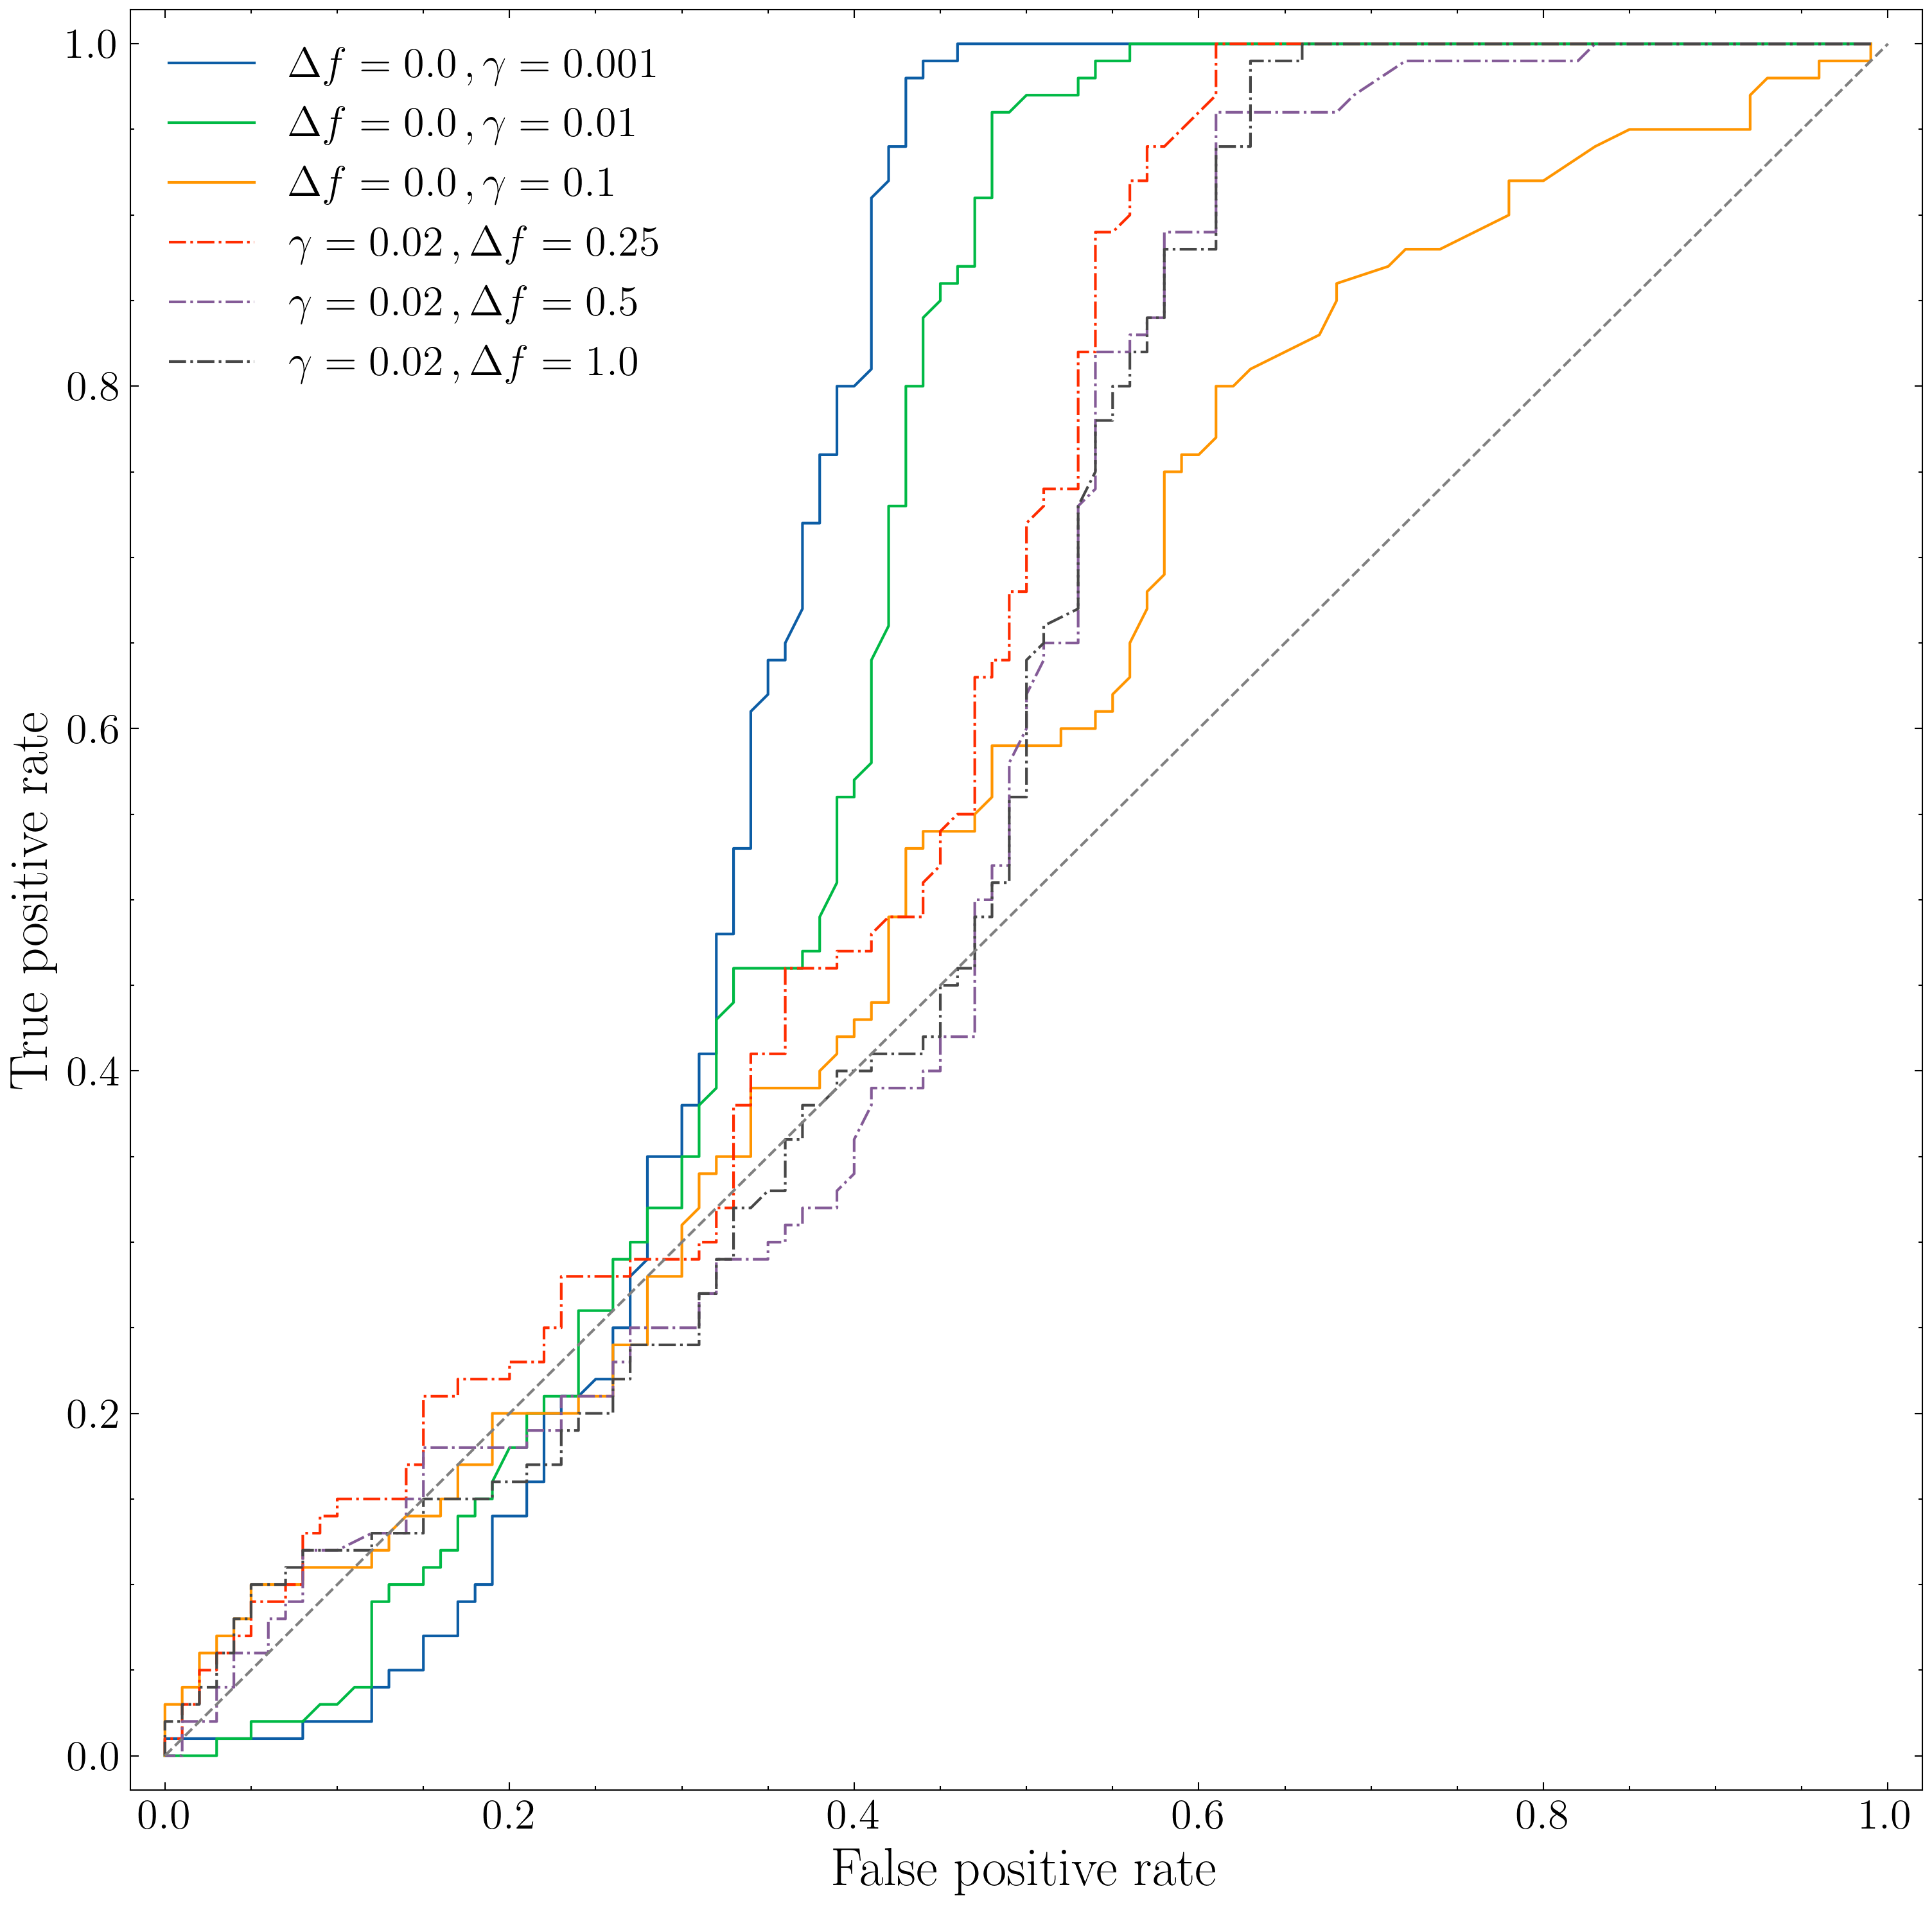
\includegraphics[width=\columnwidth]{images/4C_roccurve.png}
%DIF > 		\end{center}
%DIF > 	\caption{ROC curve over multiple noise realisations for different power line parameters. All other parameters are as specified in Table \ref{tab:parameterdescription2}. There is an evident high false alarm rate for all parameters, with a low AUC value of 0.55 for $\Delta f =0.0$, $\gamma=0.1$, and a high AUC value of 0.68 for $\Delta f =0.0$, $\gamma=0.001$. The high false alarm rate is a result of the interference not being completely removed by the ANC filter.}
%DIF > 	\label{fig:roc1}
%DIF > \end{figure}
\DIFaddbegin 


\DIFaddend \begin{figure}
	\begin{center}
		\DIFdelbeginFL %DIFDELCMD < 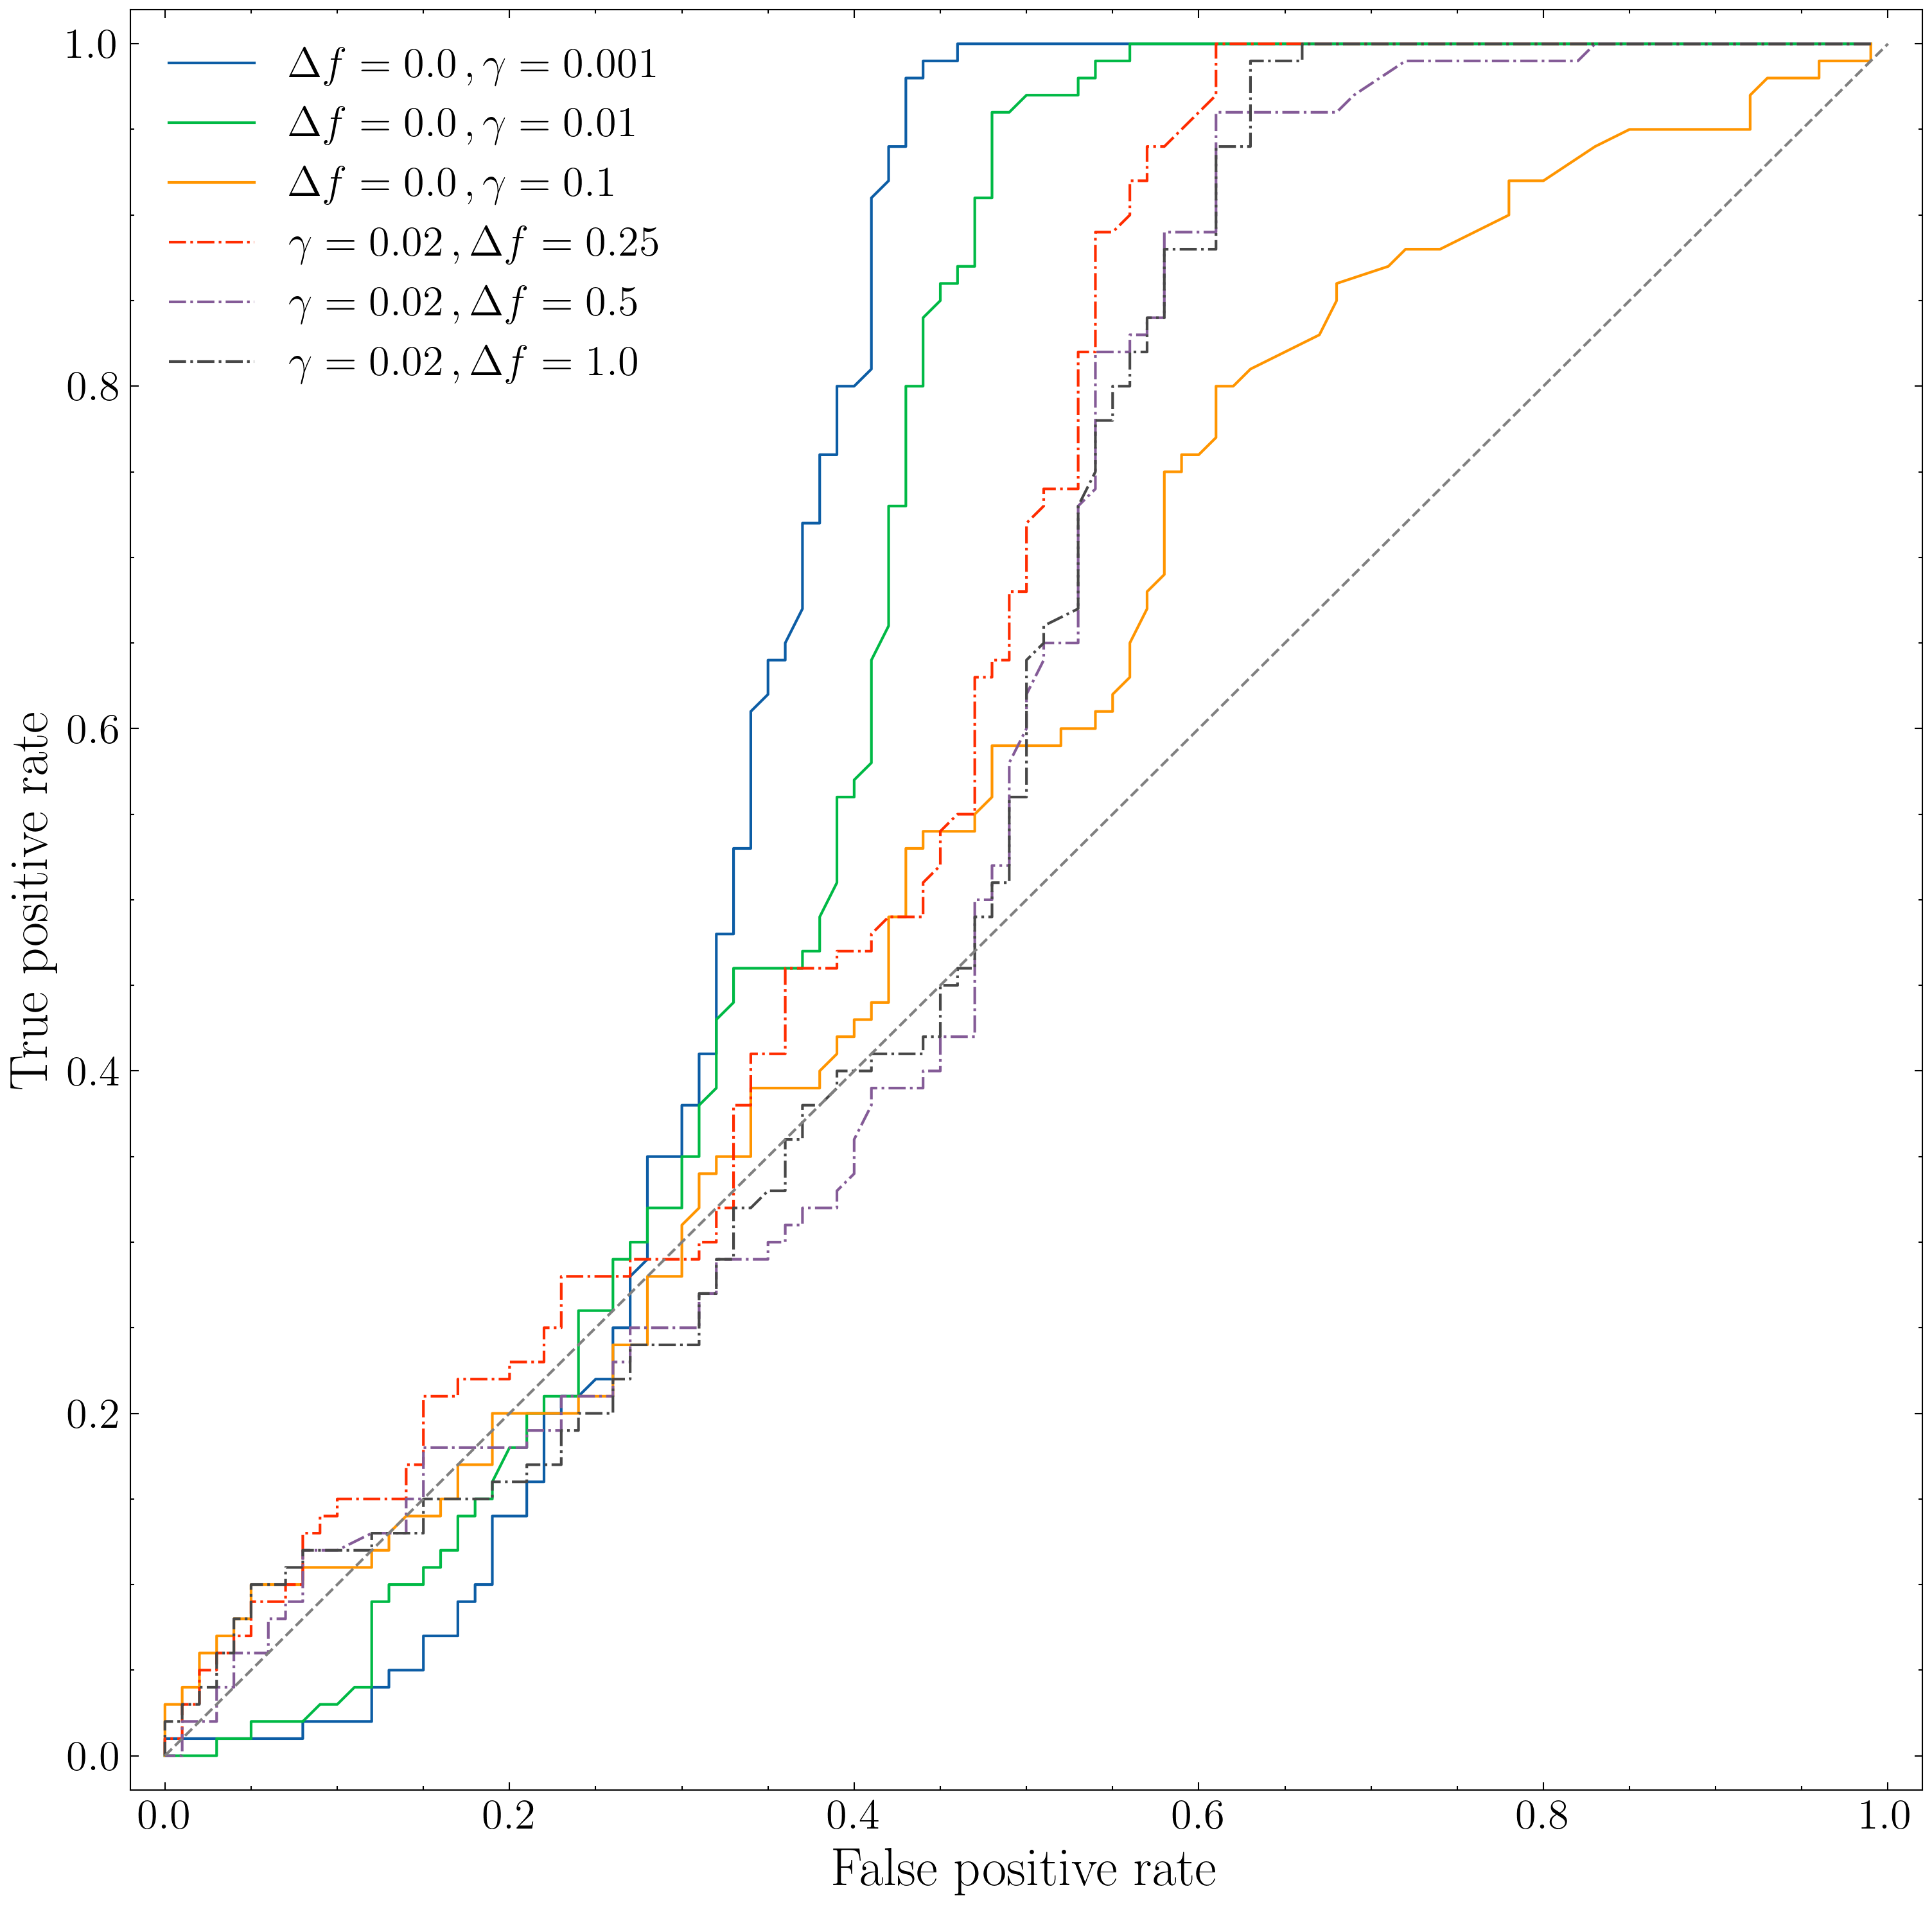
\includegraphics[width=\columnwidth]{images/4C_roccurve.png}
%DIFDELCMD < 		%%%
\DIFdelendFL \DIFaddbeginFL 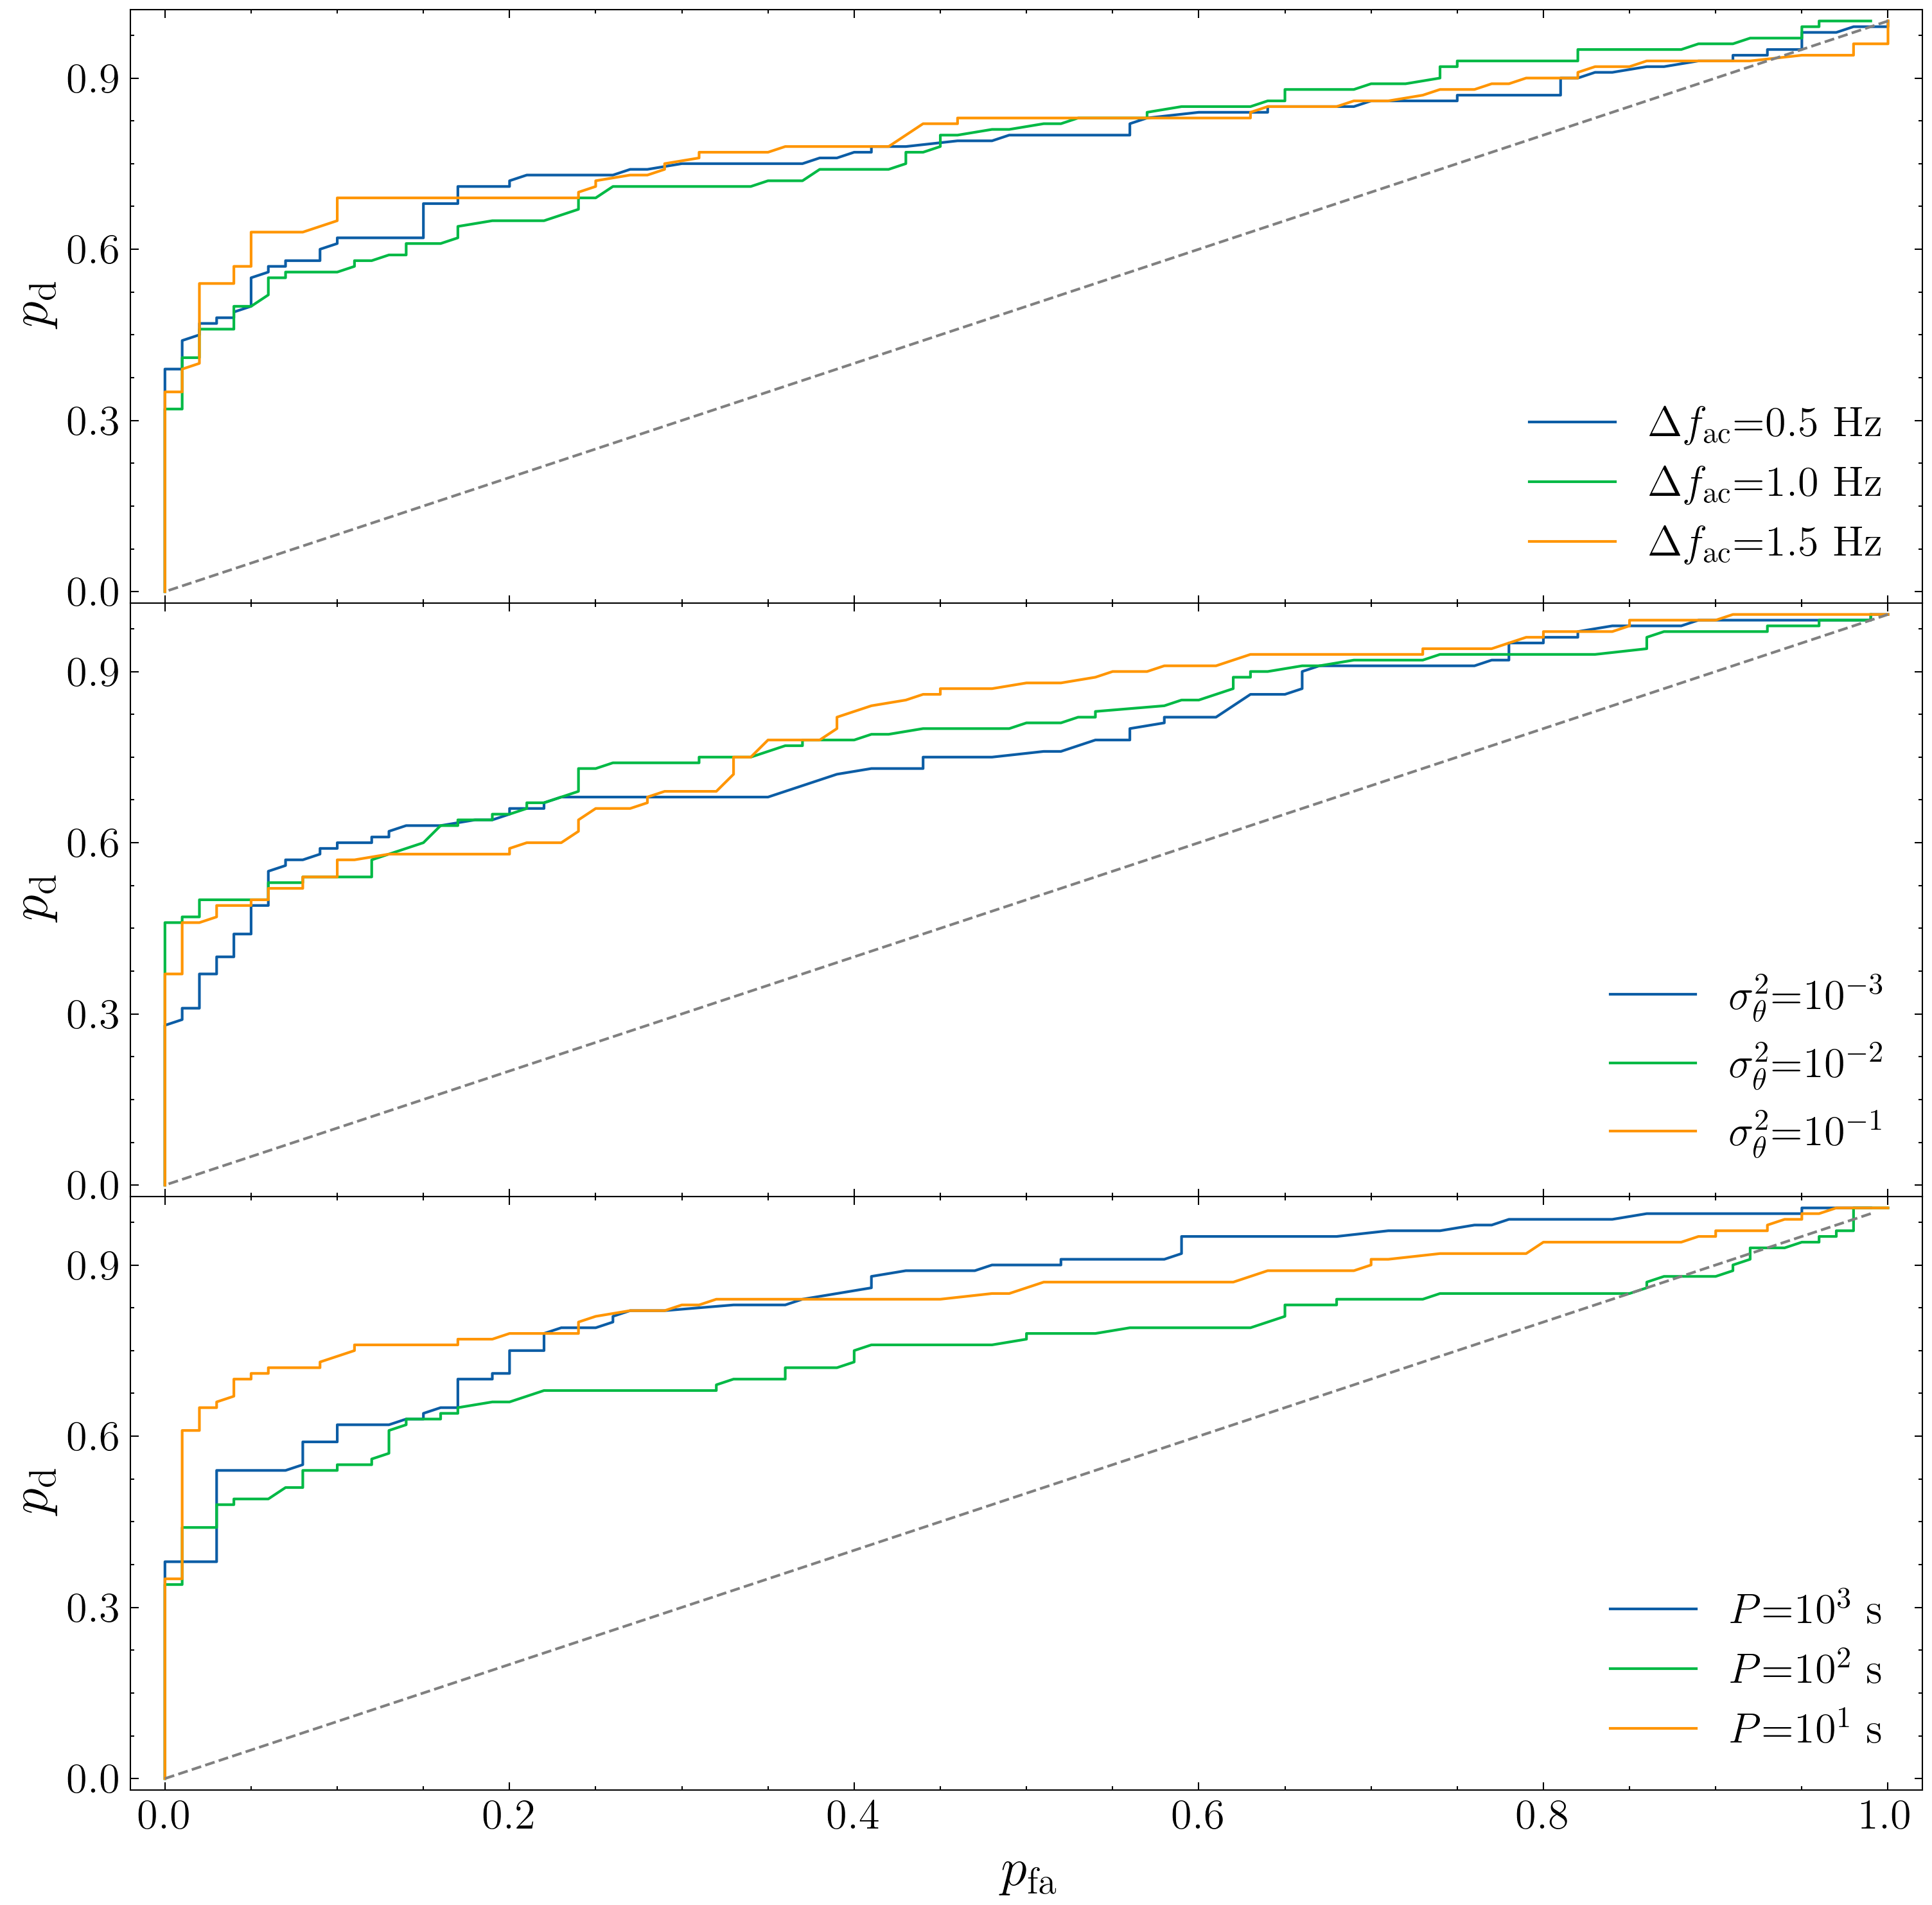
\includegraphics[width=\columnwidth]{images/roc_curve_mains_power_params}
	\DIFaddendFL \end{center}
	\caption{\DIFaddbeginFL \DIFaddFL{Detection probability $p_{\rm d}$ as a function of false alarm probability $p_{\rm fa}$ (i.e. }\DIFaddendFL ROC \DIFdelbeginFL \DIFdelFL{curve over multiple noise realisations }\DIFdelendFL \DIFaddbeginFL \DIFaddFL{curves) }\DIFaddendFL for \DIFaddbeginFL \DIFaddFL{HMM tracking of a CW signal ($h_0 / \sigma_n^2 = 0.022$) in conjunction with the ANC scheme, for }\DIFaddendFL different \DIFaddbeginFL \DIFaddFL{mains }\DIFaddendFL power \DIFdelbeginFL \DIFdelFL{line }\DIFdelendFL \DIFaddbeginFL \DIFaddFL{interference }\DIFaddendFL parameters. \DIFdelbeginFL \DIFdelFL{All other parameters are as specified in Table \ref{tab:parameterdescription2}. There is an evident high false alarm rate for all parameters}\DIFdelendFL \DIFaddbeginFL \DIFaddFL{The top panel shows different values of $\Delta f_{\rm ac}$}\DIFaddendFL , \DIFdelbeginFL \DIFdelFL{with a low AUC value }\DIFdelendFL \DIFaddbeginFL \DIFaddFL{the middle panel different values }\DIFaddendFL of \DIFdelbeginFL \DIFdelFL{0.55 for $\Delta f =0.0$}\DIFdelendFL \DIFaddbeginFL \DIFaddFL{$\sigma_{\Theta}^2$}\DIFaddendFL , \DIFdelbeginFL \DIFdelFL{$\gamma=0.1$, }\DIFdelendFL and \DIFdelbeginFL \DIFdelFL{a high AUC value }\DIFdelendFL \DIFaddbeginFL \DIFaddFL{the bottom panel different values }\DIFaddendFL of \DIFdelbeginFL \DIFdelFL{0.68 for $\Delta f =0.0$, $\gamma=0.001$}\DIFdelendFL \DIFaddbeginFL \DIFaddFL{$P$}\DIFaddendFL . The \DIFdelbeginFL \DIFdelFL{high false alarm rate is a result }\DIFdelendFL \DIFaddbeginFL \DIFaddFL{grey dashed line in all panels denotes the performance }\DIFaddendFL of \DIFaddbeginFL \DIFaddFL{a random classifier. For all panels }\DIFaddendFL the \DIFdelbeginFL \DIFdelFL{interference not being completely removed by }\DIFdelendFL \DIFaddbeginFL \DIFaddFL{curves are broadly overlaid, illustrating that }\DIFaddendFL the \DIFaddbeginFL \DIFaddFL{HMM and }\DIFaddendFL ANC \DIFdelbeginFL \DIFdelFL{filter}\DIFdelendFL \DIFaddbeginFL \DIFaddFL{scheme is resilient to different mains power parameters}\DIFaddendFL . \DIFaddbeginFL \DIFaddFL{At $p_{\rm fa} = 0.05$, the mean $p_{d}$ across the 3 curves is 0.52 (top panel), 0.48 (middle panel) and 0.58 (bottom panel). \textcolor{red}{TK: we could also label as e.g. $\Delta f_{\rm ac} / f_{\rm ac}$ as AM suggests. I personally find the absolute value with units more intuitive w.r.t the rest of the body text. Also: what do we think about having blue/green/orange curves in every panel?}}\DIFaddendFL }
	\label{fig:roc1}
\end{figure}
\DIFdelbegin \DIFdel{With the performance of the ANC and Viterbi approach established for a single example, it is of interest to explore how the algorithm performs for different power line parameters. }\DIFdelend In this section we \DIFdelbegin \DIFdel{vary $\Delta f$ and $\gamma$ to }\DIFdelend test how the \DIFdelbegin \DIFdel{combined ANC filter and Viterbi algorithm perform across multiple noise realisations}\DIFdelend \DIFaddbegin \DIFadd{ANC scheme and HMM tracker perform together as a function of the mains power parameters $\Delta f_{\rm ac}$, $\sigma_\Theta^2$ and $P$}\DIFaddend . To this end\DIFaddbegin \DIFadd{, }\DIFaddend we calculate the \DIFdelbegin \DIFdel{detection probability compared to the }\DIFdelend \DIFaddbegin \DIFadd{probability of detecting the CW signal, $p_{\rm d}$, as a function of the }\DIFaddend false alarm probability, \DIFdelbegin \DIFdel{i.e. the receiver operating characteristic (ROC ), for the Viterbi search after the data has been filtered using ANC}\DIFdelend \DIFaddbegin \DIFadd{$p_{\rm fa}$, i.e. the ROC curve $p_{\rm d} (p_{\rm fa})$}\DIFaddend . We consider \DIFdelbegin \DIFdel{two situations}\DIFdelend \DIFaddbegin \DIFadd{three numerical experiments}\DIFaddend . In the first \DIFdelbegin \DIFdel{situation we hold $\Delta f$ constant at $\Delta f =0.0$ and set $\gamma = \{ 0.001, 0.01, 0.1\}$}\DIFdelend \DIFaddbegin \DIFadd{experiment we vary $\Delta f_{\rm ac} =  \{0.5, 1.0, 1.5\}$ Hz whilst holding constant $\sigma_{\Theta}^2 = 10^{-2}$ and $P = 100 $s}\DIFaddend . In the second \DIFdelbegin \DIFdel{situation we hold $\gamma$ constant at $\gamma = 0.02$ and set  $\Delta f = \{0.25, 0.5,1.0\}$. The results are shown in Figure \ref{fig:roc1}. Whilst the underlying wandering GW frequency signal can generally be tracked well for a single noise realisation (c. f. Figure \ref{frequency tracking before and after1}), we can see that for these power line parameters , across multiple noise realisations there is a high false alarm rate. This is a consequence of the interference not being completely removed and evidences how even a small quantity of clutter noise is sufficient to corrupt the search for continuous waves. To quantify the performance with a single scalar value we consider the Area Under the Curve (AUC), a common metric used to evaluate ROC curves . The AUC can be in the range $0.5 -- 1.0$, where $\text{AUC} = 0.5$ corresponds to the }\DIFdelend \DIFaddbegin \DIFadd{experiment we vary $\sigma_{\Theta}^2 =  \{ 10^{-3}, 10^{-2}, 10^{-1}\}$ whilst holding constant $\Delta f_{\rm ac} = 1.0$ Hz and $P = 100 $s. In the third experiment we vary $P=  \{ 10, 10^2, 10^3\}$ s whilst holding constant $\Delta f_{\rm ac} = 1.0$ Hz and $\sigma_{\Theta}^2 = 10^{-2}$. For all experiments $h_0 / \sigma_n^2 = 0.022$, $f_{\rm gw}(t=0)$ is fixed to 59.9 Hz, and $N \Delta t = 800$ s. Note that despite expecting $\Delta f_{\rm ac} < 0.5$, as discussed in Section \ref{sec21}, in this Section we trial larger values of $\Delta f_{\rm ac}$ in order to provide a more difficult test for the ANC scheme and HMM tracker. All other parameters are specified in Table \ref{tab:parameterdescription1}. }\newline 


\DIFadd{Figure \ref{fig:roc1} displays the ROC curves resulting from the three numerical experiments above. In the top panel the results of the first experiment are plotted, where we set  $\Delta f_{\rm ac} = \{0.5, 1.0, 1.5\}$ Hz (blue, green and orange curves respectively). Also plotted for comparison is the }\DIFaddend performance of a random classifier (\DIFdelbegin \DIFdel{i.e. the }\DIFdelend grey dashed diagonal line\DIFdelbegin \DIFdel{in the figure)and $\text{AUC} = 1.0$ represents a perfect classifier . For the first situation with $\Delta f =0.0$ and $\gamma = \{0.001, 0.01, 0.1\}$, AUC }\DIFdelend \DIFaddbegin \DIFadd{). The performance across different $\Delta f_{\rm ac}$ values is broadly comparable, with the ROC curves generally overlaid. For all values of $\Delta f_{\rm ac}$ the ANC scheme and HMM tracker outperform a random classifier (i.e. each of the ROC curves lies above the grey dashed line). We take $p_{d}(p_{\rm fa} =0.05)$ as a scalar metric to quantify the performance of the HMM-ANC combination. For the top panel $p_{\rm d}(0.05$) }\DIFaddend = \DIFdelbegin \DIFdel{$\{0.68, 0.65,0.55\}$ respectively. For the second situation with $\gamma = 0.02$ and $\Delta f = \{0.25, 0.5,1.0\}$, AUC = $\{0.62, 0.58,0.58\}$ respectively. Whilst the method performs better than }\DIFdelend \DIFaddbegin \DIFadd{$(0.5, 0.5, 0.57)$ for $\Delta f_{\rm ac} =  \{0.5, 1.0, 1.5\}$ Hz respectively. In the middle panel the results of the second experiment are plotted, where we set  $\sigma_{\Theta}^2 =  \{ 10^{-3}, 10^{-2}, 10^{-1}\}$  (blue, green and orange curves respectively). Again the ANC scheme and HMM tracker outperform }\DIFaddend a random classifier\DIFdelbegin \DIFdel{for all parameters, }\DIFdelend \DIFaddbegin \DIFadd{, and the results are broadly consistent across different parameter values, with $p_{\rm d}(0.05$) = $(0.44,0.50,0.49)$ for $\sigma_{\Theta}^2 =  \{ 10^{-3}, 10^{-2}, 10^{-1}\}$ respectively. In }\DIFaddend the \DIFdelbegin \DIFdel{AUC values are generally low, especially for cases where the interference has a large amplitude with a long period. In Section \ref{sec:roc2} we explore the use of different parameters used for the ANC filter, including the inclusion of additional reference channels
}\DIFdelend \DIFaddbegin \DIFadd{bottom panel the results of the third experiment are plotted where we set $P=  \{ 10, 10^2, 10^3\}$ s (blue, green and orange curves respectively). Once again the scheme outperforms a random classifier and is robust to different parameter values, with $p_{\rm d}(0.05) = (0.7,0.49,0.54)$ for $P=  \{ 10, 10^2, 10^3\}$ s respectively.
}\DIFaddend 


\subsection{\DIFdelbegin \DIFdel{ROC curves vs. filter }\DIFdelend \DIFaddbegin \DIFadd{Filter }\DIFaddend parameters} \label{sec:roc2}
\begin{figure}
	\begin{center}
		\DIFdelbeginFL %DIFDELCMD < 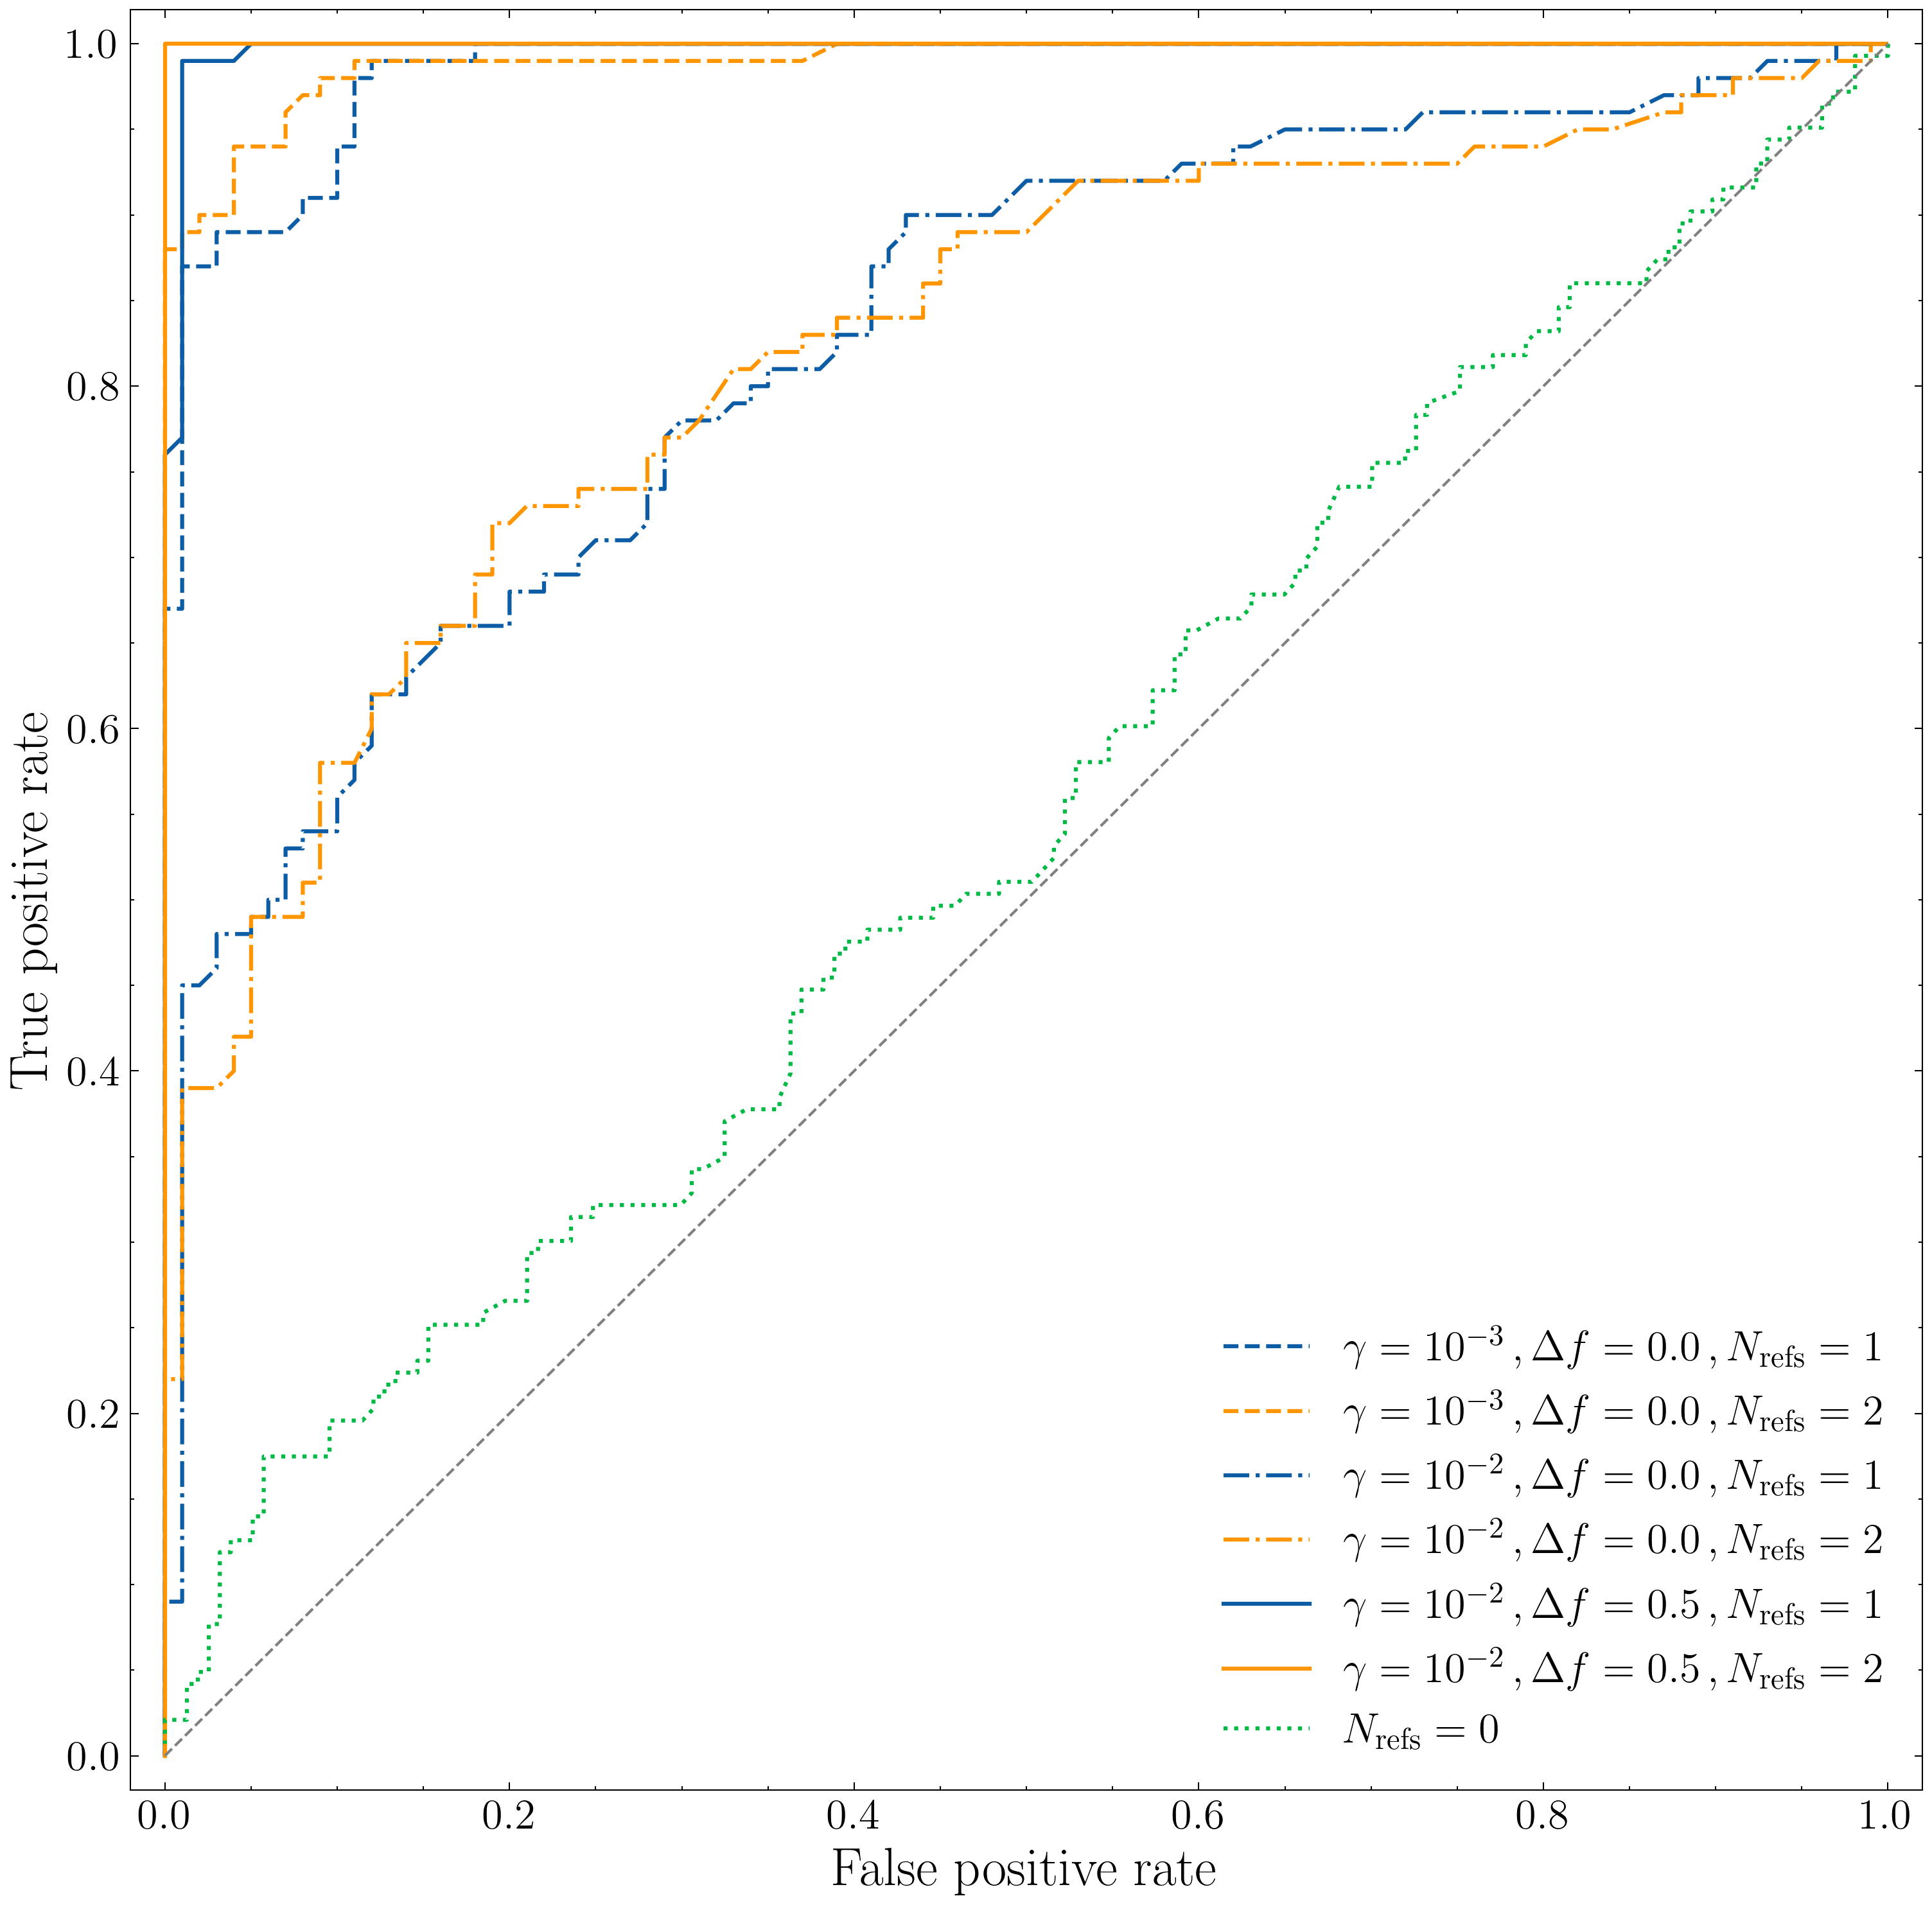
\includegraphics[width=\columnwidth]{images/4C_roccurve_multi_ref}
%DIFDELCMD < 	%%%
\DIFdelendFL \DIFaddbeginFL 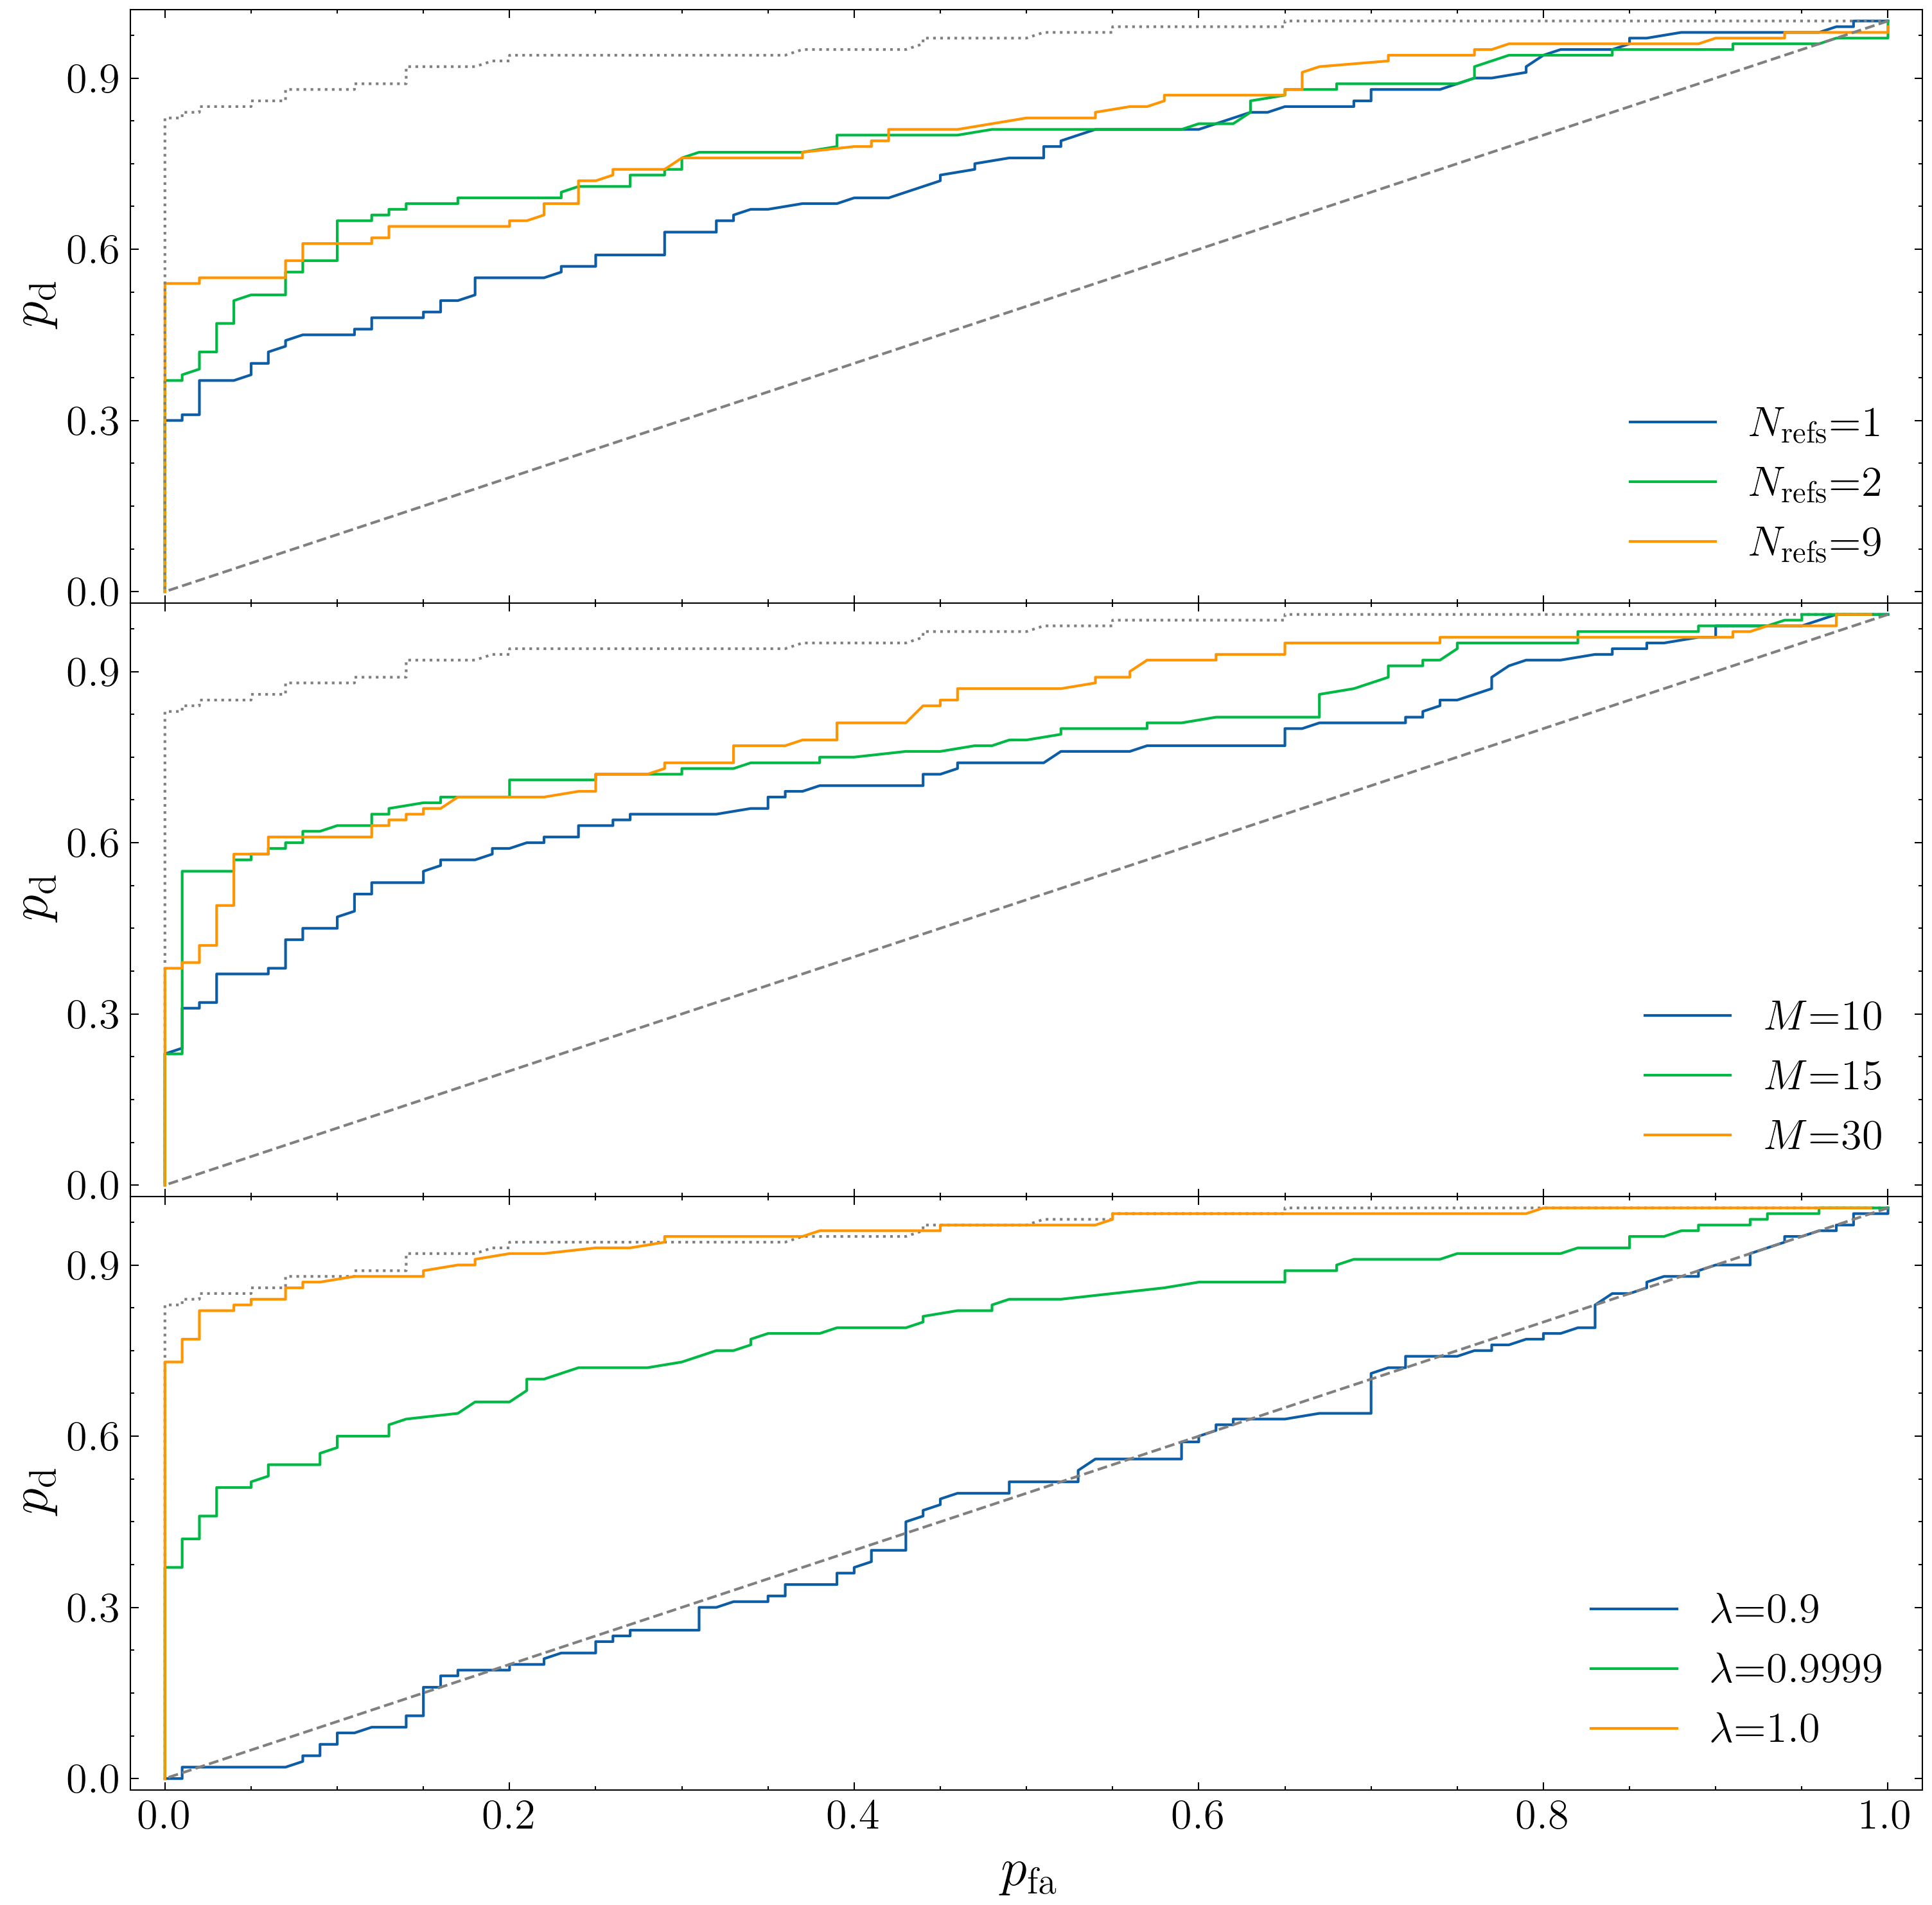
\includegraphics[width=\columnwidth]{images/roc_curve_filter_params}
	\DIFaddendFL \end{center}
	\caption{ROC \DIFdelbeginFL \DIFdelFL{curve }\DIFdelendFL \DIFaddbeginFL \DIFaddFL{curves $p_{\rm d} (p_{\rm fa})$ }\DIFaddendFL for \DIFdelbeginFL \DIFdelFL{3 }\DIFdelendFL \DIFaddbeginFL \DIFaddFL{the HMM/ANC tracking of a CW signal for }\DIFaddendFL different \DIFdelbeginFL \DIFdelFL{systems: System A with $\{ \gamma = 0.001, \Delta f = 0.0\}$, System B with $\{ \gamma = 0.01, \Delta f = 0.0\}$  and System C with $\{ \gamma = 0.01, \Delta f = 0.5\}$ (dotted, dashed, solid lines respectively)}\DIFdelendFL \DIFaddbeginFL \DIFaddFL{ANC filter parameters}\DIFaddendFL . The \DIFdelbeginFL \DIFdelFL{orange lines denote }\DIFdelendFL \DIFaddbeginFL \DIFaddFL{top panel displays }\DIFaddendFL the \DIFdelbeginFL \DIFdelFL{Viterbi search run with 2 }\DIFdelendFL \DIFaddbeginFL \DIFaddFL{ROC curves for different number of PEM }\DIFaddendFL reference channels, \DIFaddbeginFL \DIFaddFL{$N_{\rm ref}$, }\DIFaddendFL the \DIFdelbeginFL \DIFdelFL{blue lines using 1 reference channel. The green dotted line is }\DIFdelendFL \DIFaddbeginFL \DIFaddFL{middle panel different values of $M$ and }\DIFaddendFL the \DIFdelbeginFL \DIFdelFL{detection performance in the absence }\DIFdelendFL \DIFaddbeginFL \DIFaddFL{bottom panel different values }\DIFaddendFL of \DIFdelbeginFL \DIFdelFL{ANC filtering}\DIFdelendFL \DIFaddbeginFL \DIFaddFL{$\lambda$}\DIFaddendFL . \DIFdelbeginFL \DIFdelFL{The }\DIFdelendFL \DIFaddbeginFL \DIFaddFL{All panels additionally include the ROC curve for a random classifier (i.e. the lower performance limit, diagonal }\DIFaddendFL grey dashed line\DIFaddbeginFL \DIFaddFL{) and the ROC curve for the case where there }\DIFaddendFL is \DIFaddbeginFL \DIFaddFL{zero interference (i.e. }\DIFaddendFL the \DIFaddbeginFL \DIFaddFL{upper }\DIFaddendFL performance \DIFdelbeginFL \DIFdelFL{of a random classifier}\DIFdelendFL \DIFaddbeginFL \DIFaddFL{limit, grey dotted line)}\DIFaddendFL .\DIFdelbeginFL \DIFdelFL{Detection using ANC filtering consistently outperforms that without ANC filtering. ANC filtering using 2 reference channels generally outperforms that using a single reference channel.}\DIFdelendFL }
	\DIFdelbeginFL %DIFDELCMD < \label{fig:4C_roccurve_multi_ref}
%DIFDELCMD < %%%
\DIFdelendFL \DIFaddbeginFL \label{fig:roc2}
\DIFaddendFL \end{figure}
\DIFdelbegin %DIFDELCMD < \begin{table}
%DIFDELCMD < 	\centering
%DIFDELCMD < 		\resizebox{0.4\columnwidth}{!}{%
%DIFDELCMD < 		\begin{tabular}{l|ccc}
%DIFDELCMD < 			\toprule
%DIFDELCMD < 			\multicolumn{4}{c}{\hspace{6mm}System} \\
%DIFDELCMD < 			

%DIFDELCMD < 			$N_{\rm refs}$&A & B & C   \\
%DIFDELCMD < 			\hline
%DIFDELCMD < 			1& 0.975      & 0.827  & 0.987   \\
%DIFDELCMD < 			2& 0.990         & 0.822   & 0.999  \\
%DIFDELCMD < 			\bottomrule
%DIFDELCMD < 		\end{tabular}
%DIFDELCMD < 	}
%DIFDELCMD < 		%%%
%DIFDELCMD < \caption{%
{%DIFAUXCMD
\DIFdelFL{Summary of AUC values for each of the ROC curves presented in Figure \ref{fig:4C_roccurve_multi_ref}. Adding an extra PEM reference generally improves the detection performance, with the exception of system B. The AUC value for the zero PEM reference case (i.e. no ANC filtering) is $\text{AUC} = 0.55$.}}
		%DIFAUXCMD
%DIFDELCMD < \label{tab:AUC}
%DIFDELCMD < 	\end{table}
%DIFDELCMD < 

%DIFDELCMD < \begin{figure}
%DIFDELCMD < 	\begin{center}
%DIFDELCMD < 		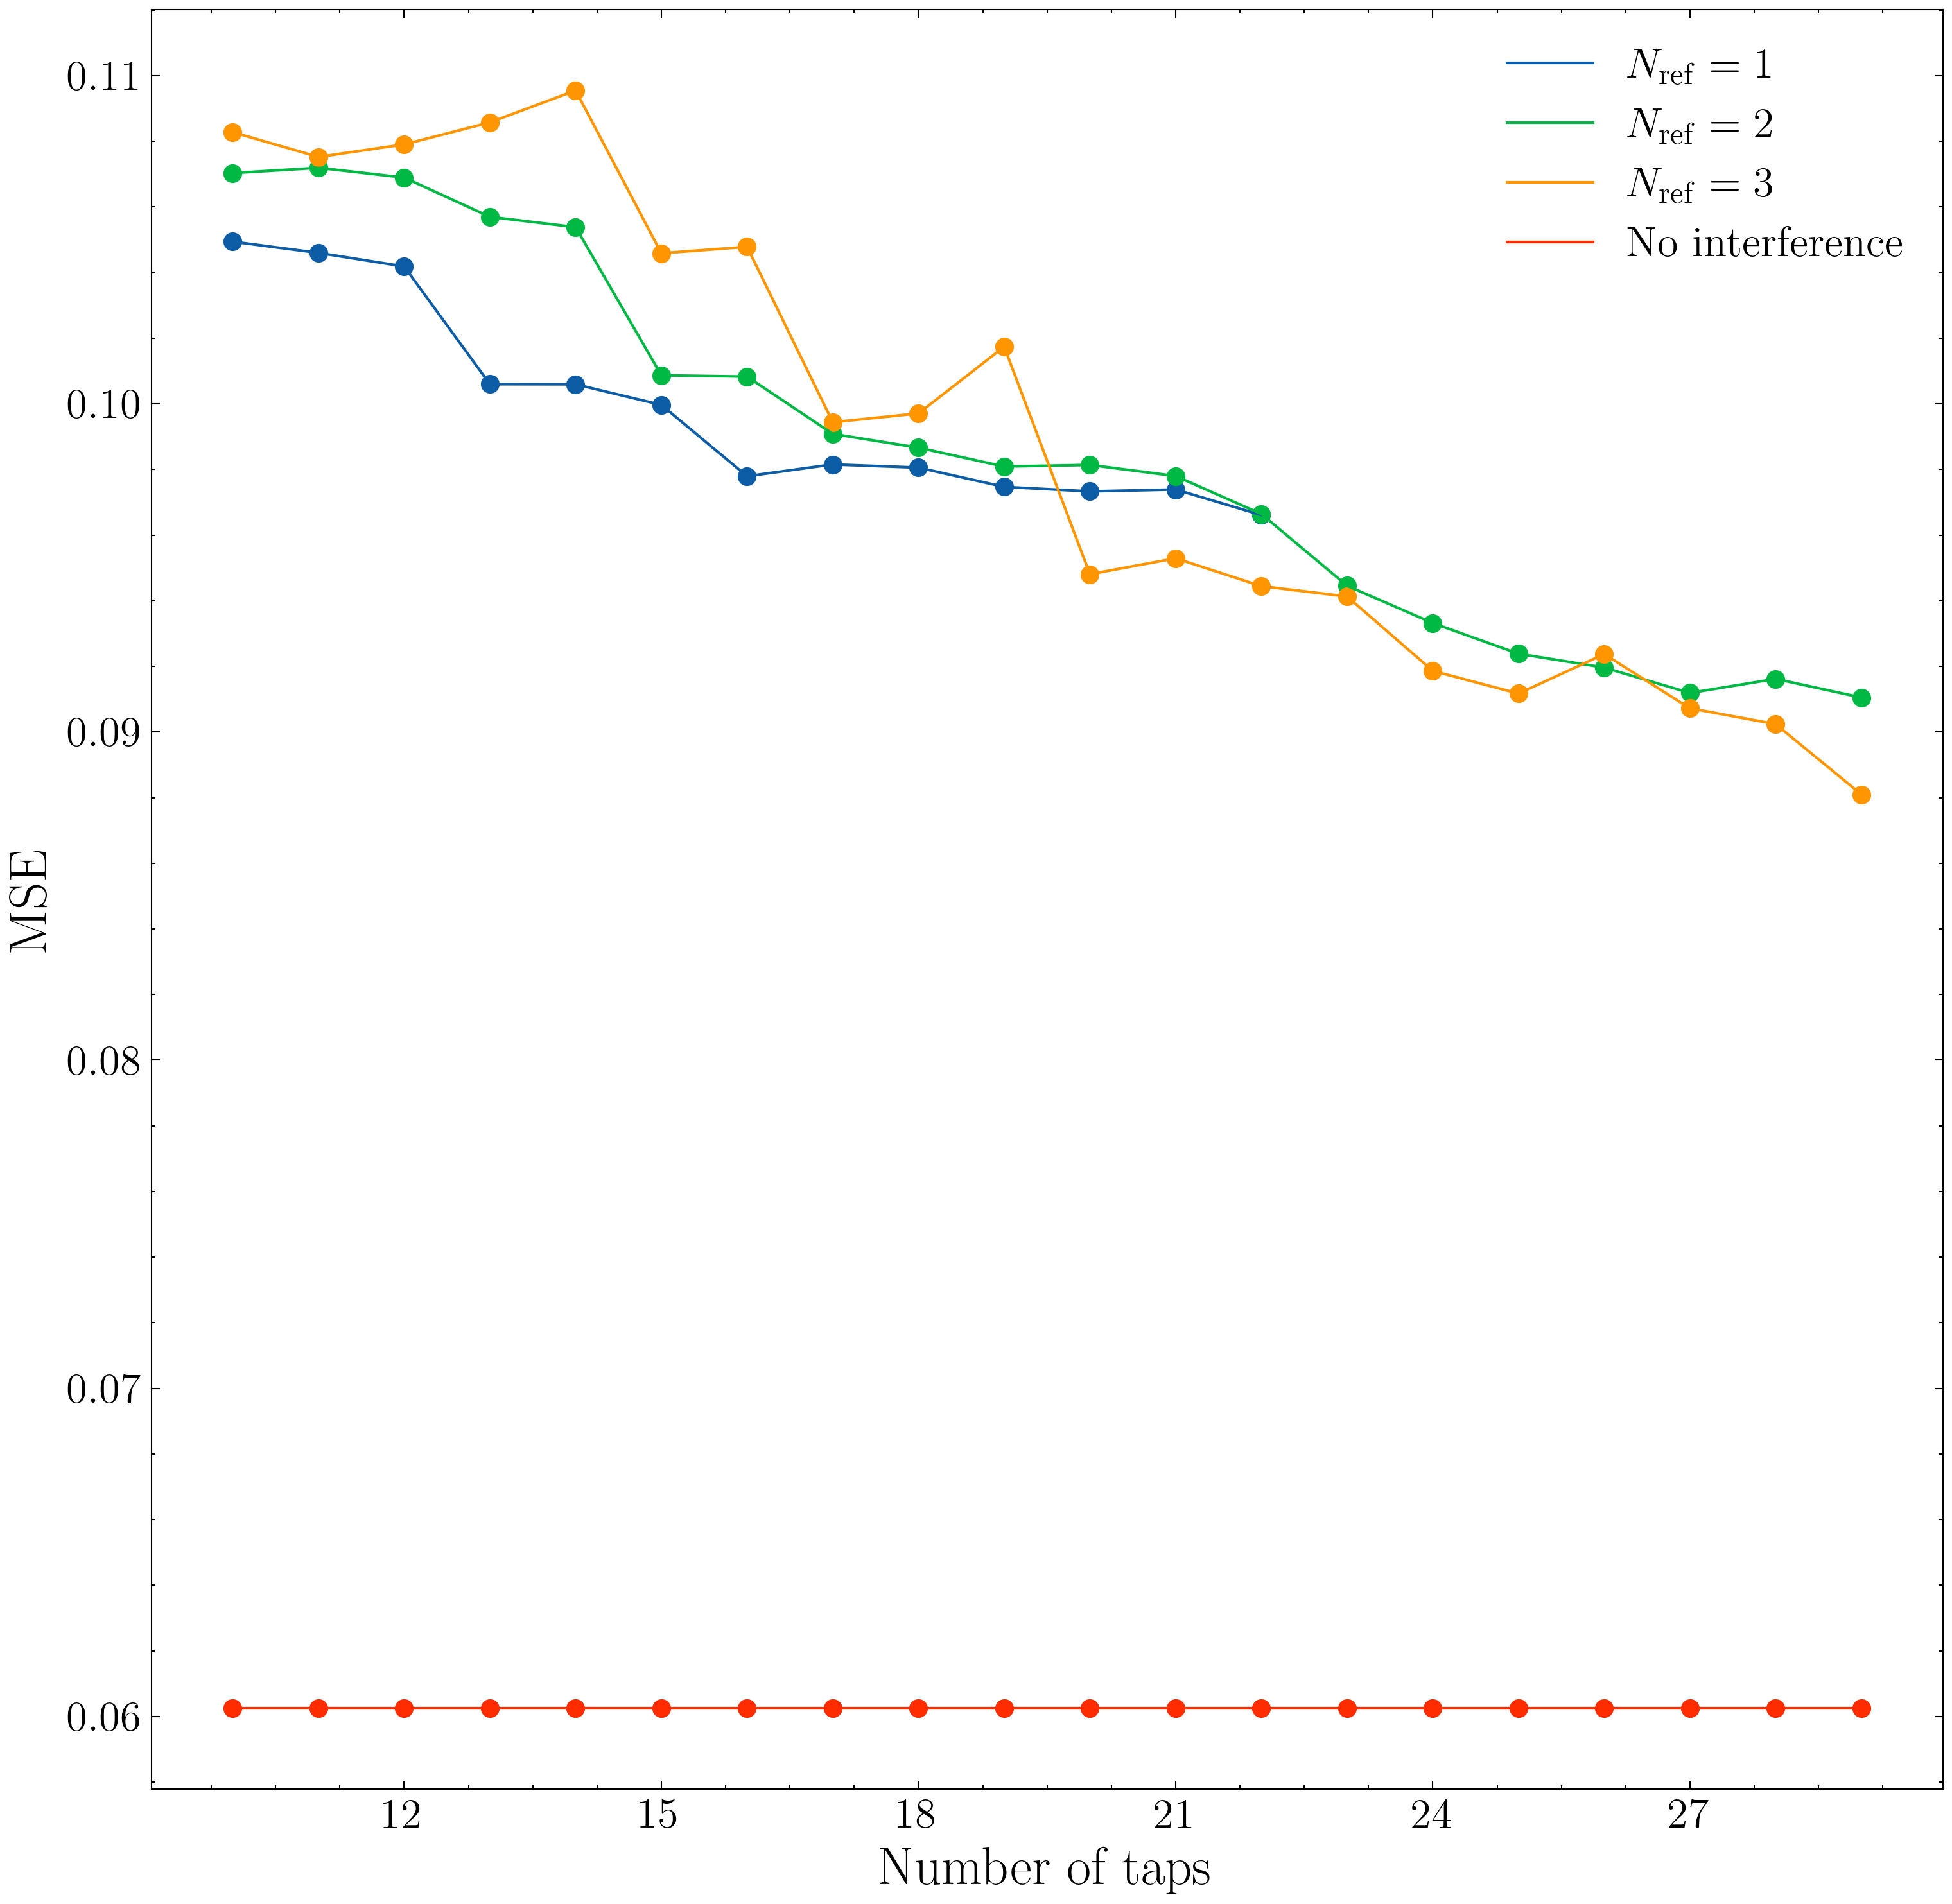
\includegraphics[width=\columnwidth]{images/taps_vs_error}
%DIFDELCMD < 	\end{center}
%DIFDELCMD < 	%%%
%DIFDELCMD < \caption{%
{%DIFAUXCMD
\DIFdelFL{Mean square error (MSE) in the Viterbi estimates of the GW wandering spin frequency for a system with $h=0.025$ and $\Delta f =0.0$ relative to the number of taps used in the FIR filter. Up to three PEM reference channels are used. The solution for the case with zero interference clutter is also shown.}}
	%DIFAUXCMD
%DIFDELCMD < \label{fig:filterorder2}
%DIFDELCMD < \end{figure}
%DIFDELCMD < 

%DIFDELCMD < %%%
\DIFdelend We have shown \DIFdelbegin \DIFdel{that the ANC filter used in conjunction with the Viterbi algorithm is effective at tracking the wandering GW spin frequency, but suffers from a high false alarm rate for the particular }\DIFdelend \DIFaddbegin \DIFadd{in Section \ref{sec:roc1} how the ANC scheme and HMM tracker are robust to different }\DIFaddend parameters of the \DIFdelbegin \DIFdel{ANC filter that we have been using}\DIFdelend \DIFaddbegin \DIFadd{mains power interference}\DIFaddend . In this \DIFdelbegin \DIFdel{Section we investigate two }\DIFdelend \DIFaddbegin \DIFadd{section we investigate different parameters of the ANC scheme itself. Specifically, we investigate three }\DIFaddend important questions:
\begin{enumerate}
	\item How does ANC benefit from multiple independent references?
	\item What order ANC filter ($M$) is required to achieve good interference cancellation? 
	\DIFaddbegin \item \DIFadd{How does ANC performance depend on $\lambda$?
}\DIFaddend \end{enumerate} 
\DIFdelbegin %DIFDELCMD < 

%DIFDELCMD < %%%
\DIFdelend Regarding the first question, the preceding validation tests on synthetic data all assumed that we have a single PEM reference voltage measurement. However, as discussed in Section \ref{sec23} in practice there are multiple PEM channels measuring power line interference for LIGO (c.f. Figure \DIFdelbegin \DIFdel{\ref{correlation_2}}\DIFdelend \DIFaddbegin \DIFadd{\ref{coherenceplot_1}}\DIFaddend ). Specifically, \DIFdelbegin \DIFdel{in the open O3a data }\DIFdelend \DIFaddbegin \DIFadd{for O3 }\DIFaddend there are 9 PEM channels \DIFdelbegin \DIFdel{for }\DIFdelend \DIFaddbegin \DIFadd{which directly measure the mains voltage at each of the }\DIFaddend LIGO-Livingston and \DIFdelbegin \DIFdel{7 PEM channels for }\DIFdelend LIGO-Hanford \DIFaddbegin \DIFadd{sites}\DIFaddend . Multiple PEM channels provided additional independent measurements of the reference voltage; it seems reasonable to suspect that these additional channels may aid the performance of the ANC filter. Indeed, ANC is commonly used with multiple reference signals in other electrical engineering applications such as noise cancelling headphones \citep{10.1121/1.5109394}, communication intelligibility \citep{KUO1996669,doi:10.1177/1084713812456906} and cardiac monitoring \citep{7755741}. \DIFdelbegin %DIFDELCMD < \newline 
%DIFDELCMD < 

%DIFDELCMD < %%%
\DIFdel{In Figure \ref{fig:4C_roccurve_multi_ref} we present the ROC curves for 3 different example systems:
}%DIFDELCMD < \begin{itemize}
\begin{itemize}%DIFAUXCMD
%DIFDELCMD < 	\item %%%
\item%DIFAUXCMD
\textbf{\DIFdel{System A}}%DIFAUXCMD
\DIFdel{. $\gamma = 10^{-3} \, , \Delta f = 0.0$. Dashed lines in the figure.
	}%DIFDELCMD < \item %%%
\item%DIFAUXCMD
\textbf{\DIFdel{System B}}%DIFAUXCMD
\DIFdel{. $\gamma = 10^{-2} \, , \Delta f = 0.0$. Dash-dotted in the figure
	}%DIFDELCMD < \item %%%
\item%DIFAUXCMD
\textbf{\DIFdel{System C}}%DIFAUXCMD
\DIFdel{. $\gamma = 10^{-2} \, , \Delta f = 0.5$. Solid lines in the figure
}
\end{itemize}%DIFAUXCMD
%DIFDELCMD < \end{itemize}
%DIFDELCMD < %%%
\DIFdel{For each system we compute the ROC curve over multiple noise realisations for both one and two reference channels (blue, and orange lines respectively). This gives us six total ROC curve solutions. For comparison we also plot the case where we run the Viterbi search for one of the example systems, but with zero PEM references (dotted green line). The specific AUC values for each ROC curve are reported in Table \ref{tab:AUC}. }%DIFDELCMD < \newline 
%DIFDELCMD < 

%DIFDELCMD < %%%
\DIFdel{We can see that for all example systems the detection probability is high with respect to the false alarm probability. The detection probability using ANC filtering is greater than without ANC filtering for all systems (i.e. the orange and blue lines are exclusively above the green dotted line). Specifically the for the zero filtering case AUC$=0.54$, whilst all cases which use ANC filtering have AUC$\ge 0.82$ and as high as AUC$=0.99$. The inclusion of an additional reference channel improves the detection probability for Systems A and C, with the AUC values rising from 0.975 to 0.990 for System A and from $0.987$ to $0.999$ for System B. No improvement is observed for System B, with AUC$=0.827$ for $N_{\rm ref} =1$ and AUC$=0.822$ for $N_{\rm ref} =2$. The lack of improvement for System B when using two PEM references suggests that for these parameters a single reference is sufficient to capture the dynamics of the interference clutter. }%DIFDELCMD < \newline  %%%
\footnote{%DIFDELCMD < \tiny %%%
\DIFdel{\textcolor{red}{TK: Why are these results so different to Figure 8? Has the strain amplitude changed? Need to check with Sofia}}%DIFDELCMD < \normalsize%%%
}
%DIFAUXCMD
\addtocounter{footnote}{-1}%DIFAUXCMD
%DIFDELCMD < 

%DIFDELCMD < %%%
\DIFdel{Regarding the }\DIFdelend \DIFaddbegin \DIFadd{For the }\DIFaddend second question, the order of the filter, i.e. the number of taps, is a parameter that can be freely chosen in ARLS. \DIFdelbegin \DIFdel{It is important to consider the filter's robustness to the choice of $M$. }\DIFdelend Generally an increased number of taps is expected to improve the performance of the filter due to the increased model complexity. However, this comes at an increased computational cost and also an increased latency. For real time applications tracking the wandering of the GW frequency it is important to minimize both of these variables. In \DIFdelbegin \DIFdel{Figure  \ref{fig:filterorder2} we plot the mean squared error (MSE) in the GW frequency estimated by Viterbi compared to the true spin-wandering frequency, averaged over multiple noise realisations. We set the system to have $h=0.025$ and $\Delta f =0.0$ and consider up to three PEM reference channels. As a reference we also plot the error in the Viterbi estimates for the case where there is no interference clutter and so no ANC is required. We can see that generally the accuracy improves with an increased number of taps. When }\DIFdelend \DIFaddbegin \DIFadd{this work we explicitly specify the number of taps; we note that adaptive tap length methods are also available \mbox{%DIFAUXCMD
\citep[e.g.][]{1326385,KAR2017422,KAR2020107043}}\hskip0pt%DIFAUXCMD
. Regarding the third question, the use of the forgetting factor $\lambda$ allows ARLS to handle non-stationary systems, neglecting older data in favour of more recent data. This is useful for cases where the model parameters are time-varying, enabling more rapid convergence and effective tracking. In the case when $\lambda = 1$, ARLS has infinite memory and so exhibits good stability and low misadjustment. However the tracking capability can be reduced for non-stationary systems. Conversely, $\lambda < 1$ improves the tracking at the expense of reduced stability and increased misadjustment \mbox{%DIFAUXCMD
\citep{Ciochina5206117}}\hskip0pt%DIFAUXCMD
. In this paper we run ARLS using a specific value for $\lambda$, but note that adaptive $\lambda$ algorithms are also available \mbox{%DIFAUXCMD
\citep{app12042077,1468506,4639569}}\hskip0pt%DIFAUXCMD
. }\newline 



\DIFadd{Figure \ref{fig:roc2} displays the ROC curves for different values of the number of PEM references ($N_{\rm ref}$, top panel), }\DIFaddend $M$ \DIFdelbegin \DIFdel{is small the $N_{\rm ref} =1$ solution generally outperforms the high }\DIFdelend \DIFaddbegin \DIFadd{(middle panel) and $\lambda$ (bottom panel). All mains power interference parameters are as specified in Table \ref{tab:parameterdescription1}. Also plotted for comparison in every panel is the ROC curve of a random classifier (grey dashed diagonal line) and the ROC curve when $c(t) = 0$ (grey dotted line). The zero interference case is included to provide a reference on the performance upper limit. }\newline 

\DIFadd{The top panel plots the ROC curves for $N_{\rm ref} = \{ 1,2,9 \}$ (blue, green and orange curves respectively). The detection probability $p_{\rm pd} (0.05) = \{ 0.38,0.52,0.55 \}$ for each of the respective }\DIFaddend $N_{\rm ref}$\DIFdelbegin \DIFdel{solutions; in this regime the number of taps is sufficiently small to not be able to take advantage of }\DIFdelend \DIFaddbegin \DIFadd{. For comparison, in }\DIFaddend the \DIFdelbegin \DIFdel{increased information provided by the additional reference channels. Conversely as the number of taps increases , the $N_{\rm ref} =3$ becomes the best performing solution. We note that rather than explicitly specifying the number of taps, adaptive tap length methods that automatically update the number of taps used are also available \mbox{%DIFAUXCMD
\citep[e.g.][]{1326385,KAR2017422,KAR2020107043}}\hskip0pt%DIFAUXCMD
. }\DIFdelend \DIFaddbegin \DIFadd{zero interference case $p_{\rm pd}(0.05) = 0.85$. It is evident that $N_{\rm ref} > 1$ are generally an improvement over $N_{\rm ref} = 1$. However, the improvement of $N_{\rm ref} =9$ over $N_{\rm ref} =2$ is more modest. This suggests that the inclusion of additional reference PEM channels quickly reaches a point of diminishing returns where the interference is well-captured by a few reference channels, and adding more references beyond this point does not improve the effectiveness of the filter. The middle panel plots $M = \{10,15,30\}$ (blue, green, and orange curves respectively). The detection probability $p_{\rm pd} (0.05) = \{0.37, 0.57, 0.58\}$ for each respective $M$. Analogous to the top panel, increasing $M$ generally increases the detection probability, but the performance quickly saturates such that the ROC curves for $M=15$ and $M=30$ are highly comparable. In the bottom panel we plot $\lambda = \{1,2,9\}$ (blue, green, orange curves respectively), which have respective $p_{\rm pd} (0.05) = \{0.38, 0.52, 0.55\}$. A clear hierarchy is evident whereby larger values of $\lambda$ increase the detection probability. For the synthetic data in this paper $\lambda=1$ is advantageous for detection since the interference is quasi-stationary (c.f. Equation \ref{eq:clutterequation}). Consequently, discounting older data with $\lambda < 1$ inhibits the ability of the ANC scheme to filter out the interference. We defer investigation of non-stationary interference (c.f. Equation \ref{eq:vclutter}) to a future work. For application to real astrophysical data $\lambda$ will need to be selected optimally e.g. \mbox{%DIFAUXCMD
\citep{6349749}}\hskip0pt%DIFAUXCMD
. 
}\DIFaddend 


%DIF > \begin{figure}
%DIF > 	\begin{center}
%DIF > 		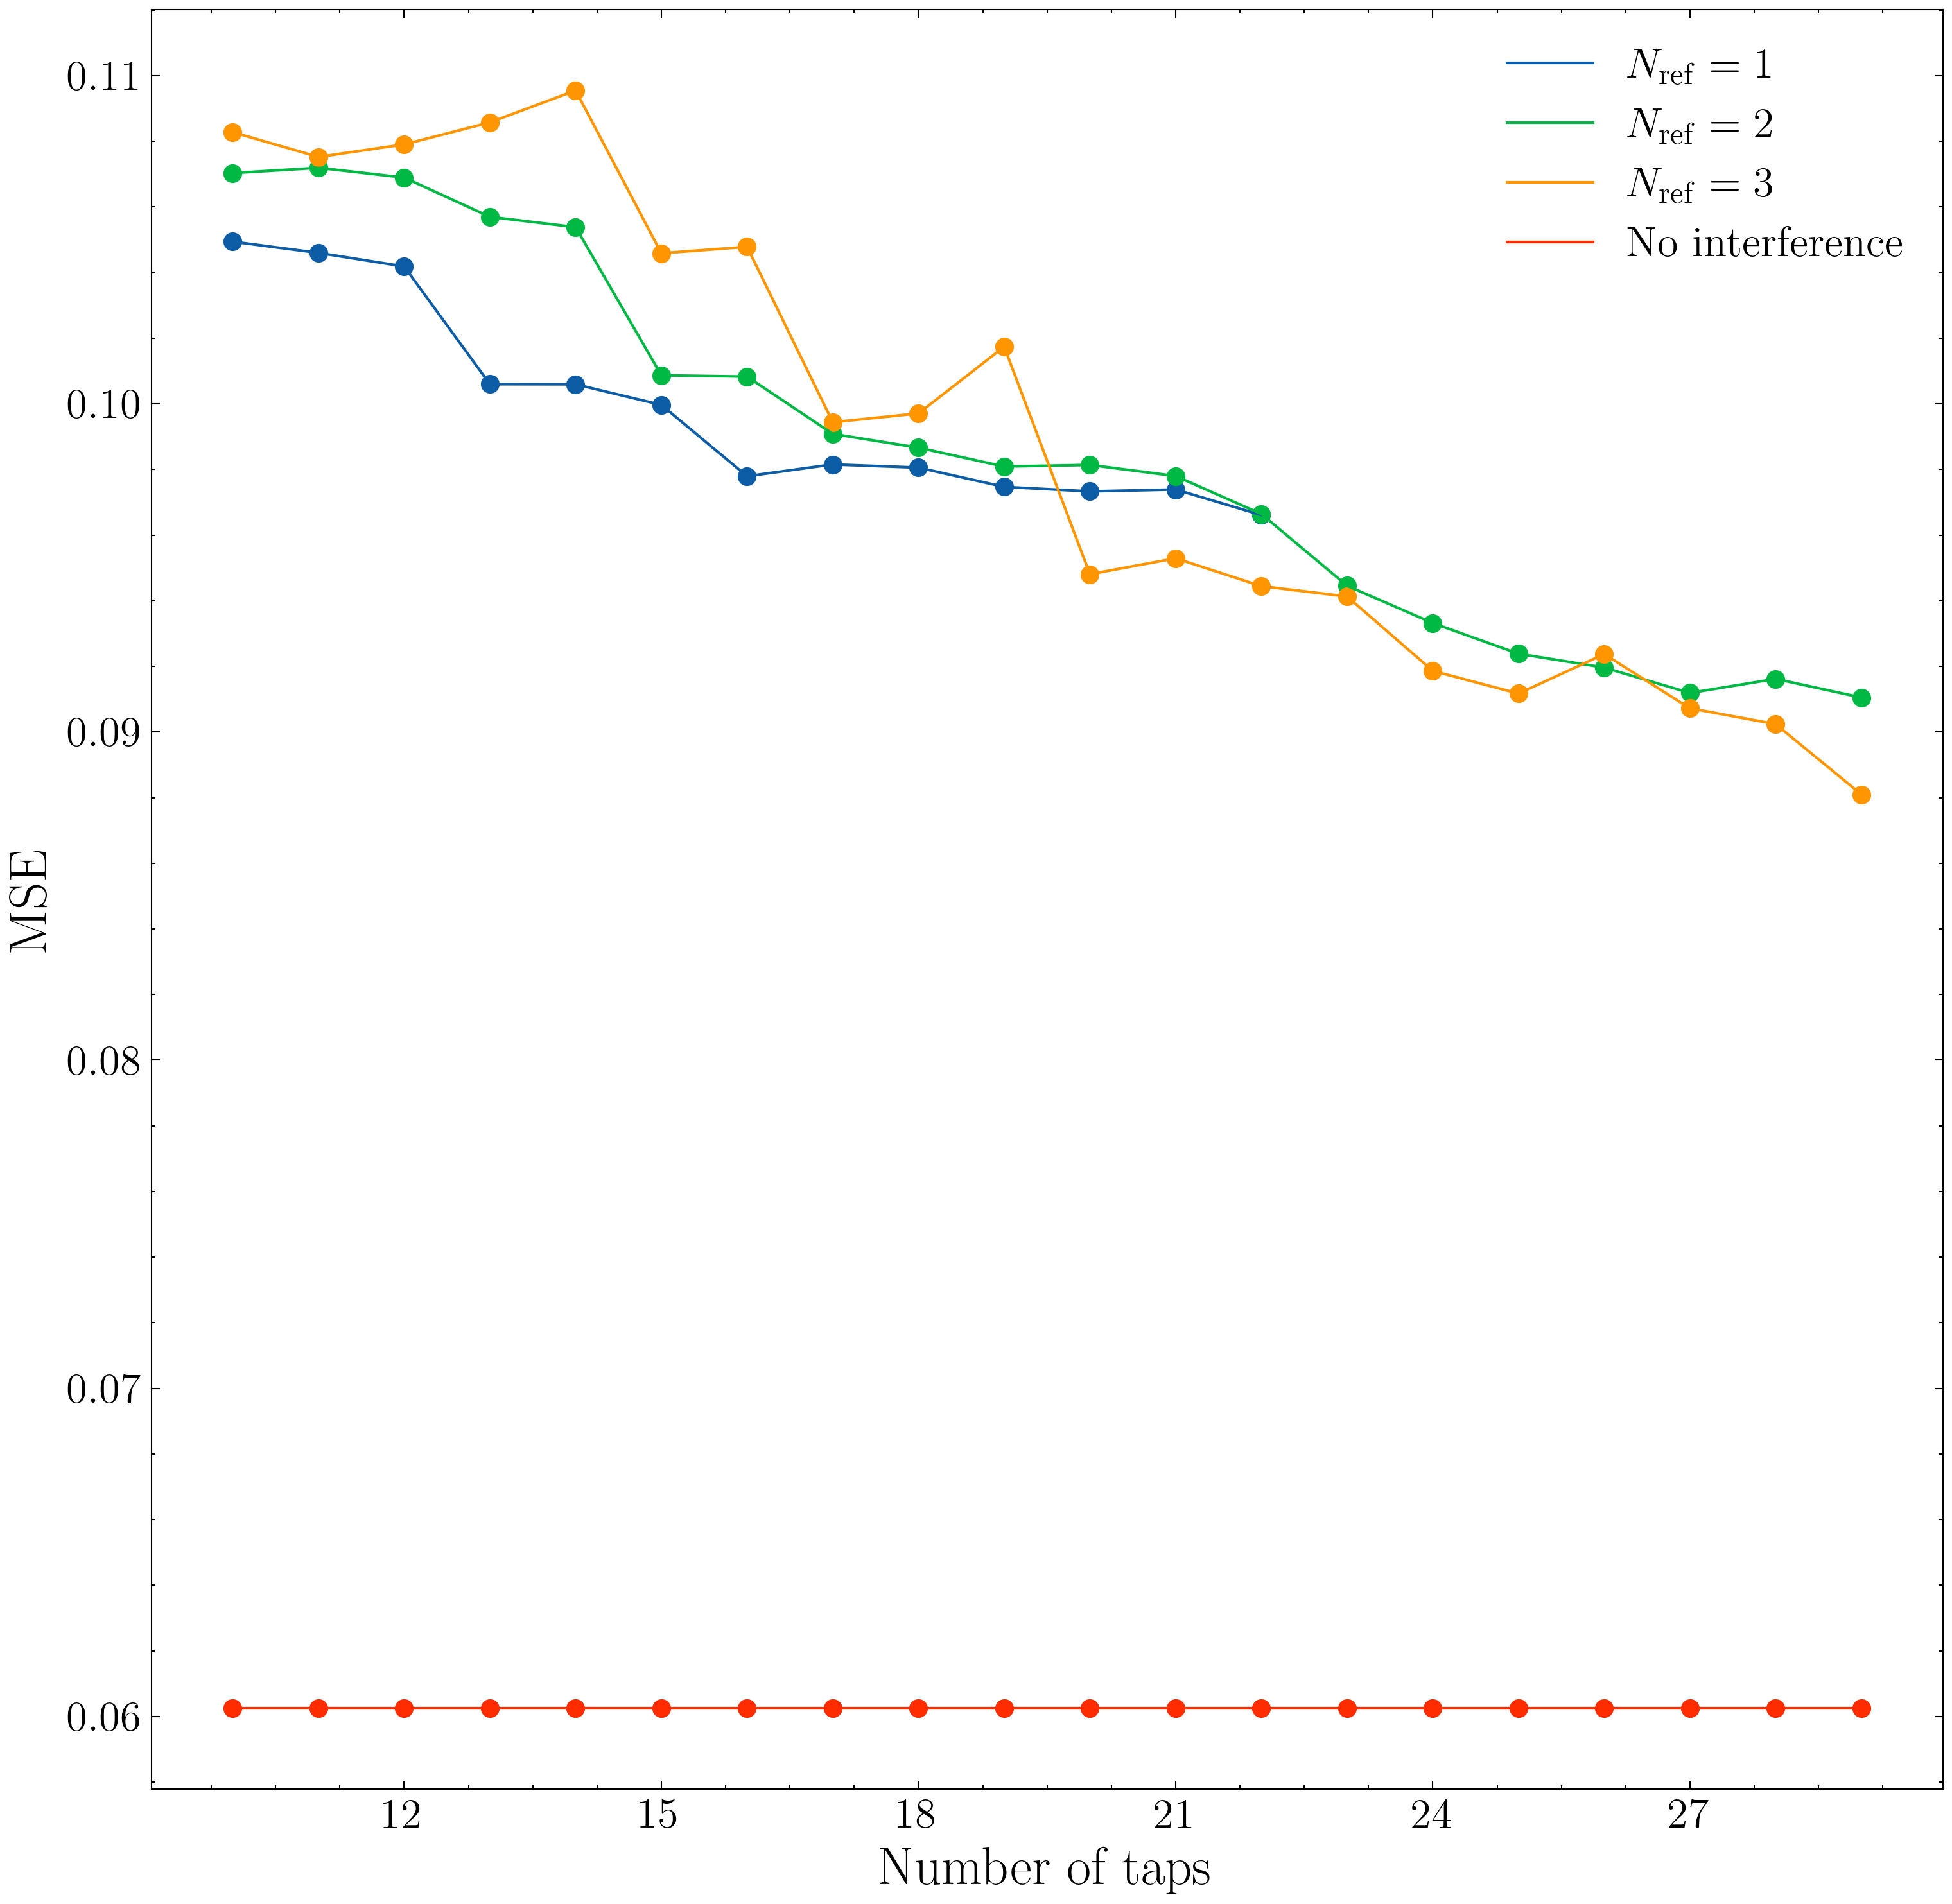
\includegraphics[width=\columnwidth]{images/taps_vs_error}
%DIF > 	\end{center}
%DIF > 	\caption{Mean square error (MSE) in the Viterbi estimates of the GW wandering spin frequency for a system with $h=0.025$ and $\Delta f =0.0$ relative to the number of taps used in the FIR filter. Up to three PEM reference channels are used. The solution for the case with zero interference clutter is also shown.}
%DIF > 	\label{fig:filterorder2}
%DIF > \end{figure}
\DIFaddbegin 


%DIF > We have shown that the ANC filter used in conjunction with the Viterbi algorithm is effective at tracking the wandering GW spin frequency, but suffers from a high false alarm rate for the particular parameters of the ANC filter that we have been using. 
%DIF > 
%DIF > 
%DIF > 
%DIF > 
%DIF > 
%DIF > 
%DIF > 
%DIF > 
%DIF > 
%DIF > 
%DIF > The results are presented in Figure \ref{fig:roc2}
%DIF > 
%DIF > 
%DIF > 
%DIF > 
%DIF > 
%DIF > 










%DIF > In Figure \ref{fig:4C_roccurve_multi_ref} we present the ROC curves for 3 different example systems:
%DIF > \begin{itemize}
%DIF > 	\item \textbf{System A}. $\gamma = 10^{-3} \, , \Delta f = 0.0$. Dashed lines in the figure.
%DIF > 	\item \textbf{System B}. $\gamma = 10^{-2} \, , \Delta f = 0.0$. Dash-dotted in the figure
%DIF > 	\item \textbf{System C}. $\gamma = 10^{-2} \, , \Delta f = 0.5$. Solid lines in the figure
%DIF > \end{itemize}
%DIF > For each system we compute the ROC curve over \textbf{multiple noise realisations} for both one and two reference channels (blue, and orange lines respectively). This gives us six total ROC curve solutions. For comparison we also plot the case where we run the Viterbi search for one of the example systems, but with zero PEM references (dotted green line). The specific AUC values for each ROC curve are reported in Table \ref{tab:AUC}. \newline 

%DIF > We can see that for all example systems the detection probability is high with respect to the false alarm probability. The detection probability using ANC filtering is greater than without ANC filtering for all systems (i.e. the orange and blue lines are exclusively above the green dotted line). Specifically the for the zero filtering case AUC$=0.54$, whilst all cases which use ANC filtering have AUC$\ge 0.82$ and as high as AUC$=0.99$. The inclusion of an additional reference channel improves the detection probability for Systems A and C, with the AUC values rising from 0.975 to 0.990 for System A and from $0.987$ to $0.999$ for System B. No improvement is observed for System B, with AUC$=0.827$ for $N_{\rm ref} =1$ and AUC$=0.822$ for $N_{\rm ref} =2$. The lack of improvement for System B when using two PEM references suggests that for these parameters a single reference is sufficient to capture the dynamics of the interference clutter. \newline  \footnote{\tiny \textcolor{red}{TK: Why are these results so different to Figure 8? Has the strain amplitude changed? Need to check with Sofia}\normalsize}




%DIF > 
%DIF > Figure  \ref{fig:filterorder2} we plot the mean squared error (MSE) in the GW frequency estimated by Viterbi compared to the true spin-wandering frequency, averaged over \textbf{multiple noise realisations}. We set the system to have $h=0.025$ and $\Delta f =0.0$ and consider up to three PEM reference channels. As a reference we also plot the error in the Viterbi estimates for the case where there is no interference clutter and so no ANC is required. We can see that generally the accuracy improves with an increased number of taps. When $M$ is small the $N_{\rm ref} =1$ solution generally outperforms the high $N_{\rm ref}$ solutions; in this regime the number of taps is sufficiently small to not be able to take advantage of the increased information provided by the additional reference channels. Conversely as the number of taps increases, the $N_{\rm ref} =3$ becomes the best performing solution. 
%DIF > 








\DIFaddend %\begin{equation}
%	{\rm MSE}=E_{\rm emp} \left [(\sum_{i=0}^{KN}e_i^2)/(KN+1) \right ]
%\end{equation}
%where we use $E_{\rm emp} [X]$ to denote the empirical mean of a quantity $X$ over 500 simulations. \textcolor{red}{TK: confirm this equations is correct and what are K/N in the updated notation?}. The MSE as a function of the number of taps $M$ is shown in Fig \ref{mse vs tap} for a system with $|H(w)|=3$ and $\rm{SNR}_{\rm in}=0.02$. We can see that initially as the number of taps increases from the MSE deceases, finidng a minimum at around $M=64$. This is due to the narrower bandwidth enabling a sharper filter to remove more of the interference. Beyond this point the MSE starts to increase. Now the increased sharpness of the filter is hampered by the time delay from using too many taps and the filter is not able to track the frequency with a sufficiently small latency. 

%With the performance of the ANC and Viterbi approach established for a single example, it is of interest to explore how the algorithm performs for different power line parameters. In this section we vary $\Delta f$ and $\gamma$ to test the ANC and Viterbi performance for multiple noise realisations. To this end we calculate the detection probability compared to the false alarm probability, i.e. the receiver operating characteristic (ROC), for the Viterbi search after ANC. 
%
%
%In this paper we address two important questions 
%
%
%We investigate this by computing the 
%mean square difference between the signal after applying the ANC with the signal without interference as function of the order. 


%\begin{figure}
%	\begin{center}
%		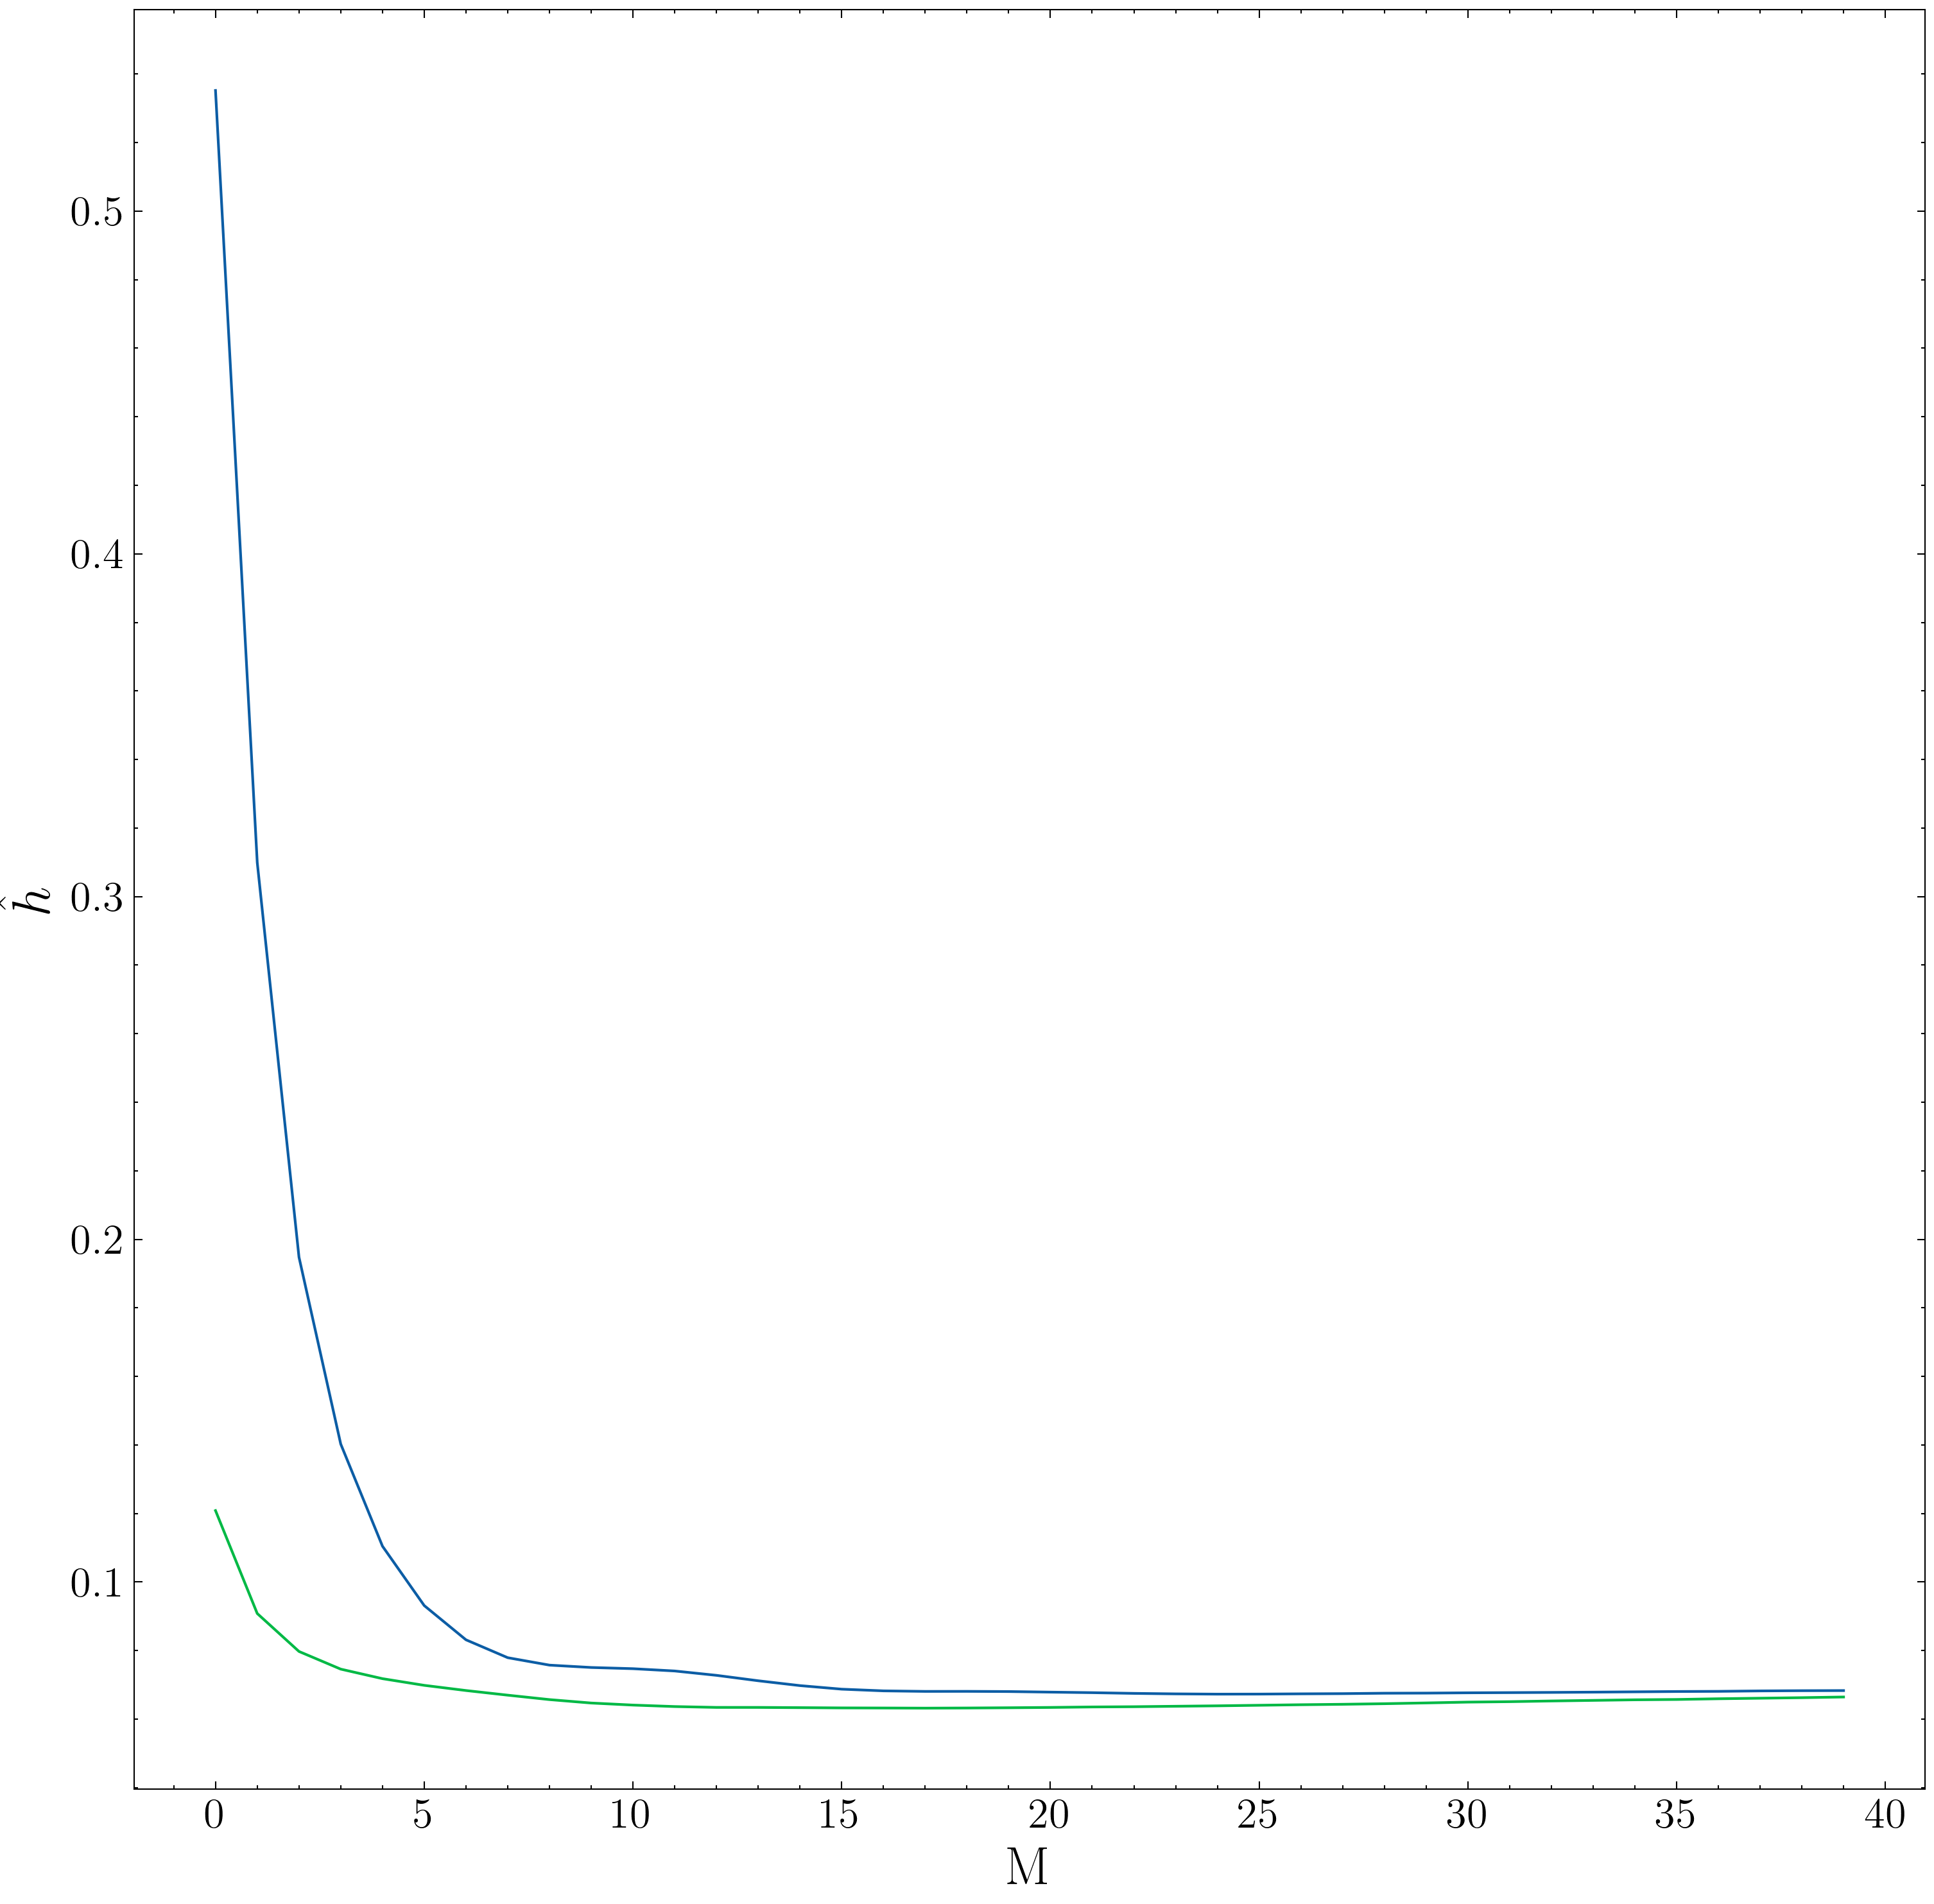
\includegraphics[width=\columnwidth]{images/filter_order.png}
%	\end{center}
%	\caption{\textcolor{red}{TK: filter order. From filter\_order\_experiments.mat. Maybe we should update this for an MSE after Viterbi?}}
%	\label{fig:filterorder}
%\end{figure}













%\begin{figure}
%	\begin{center}
%		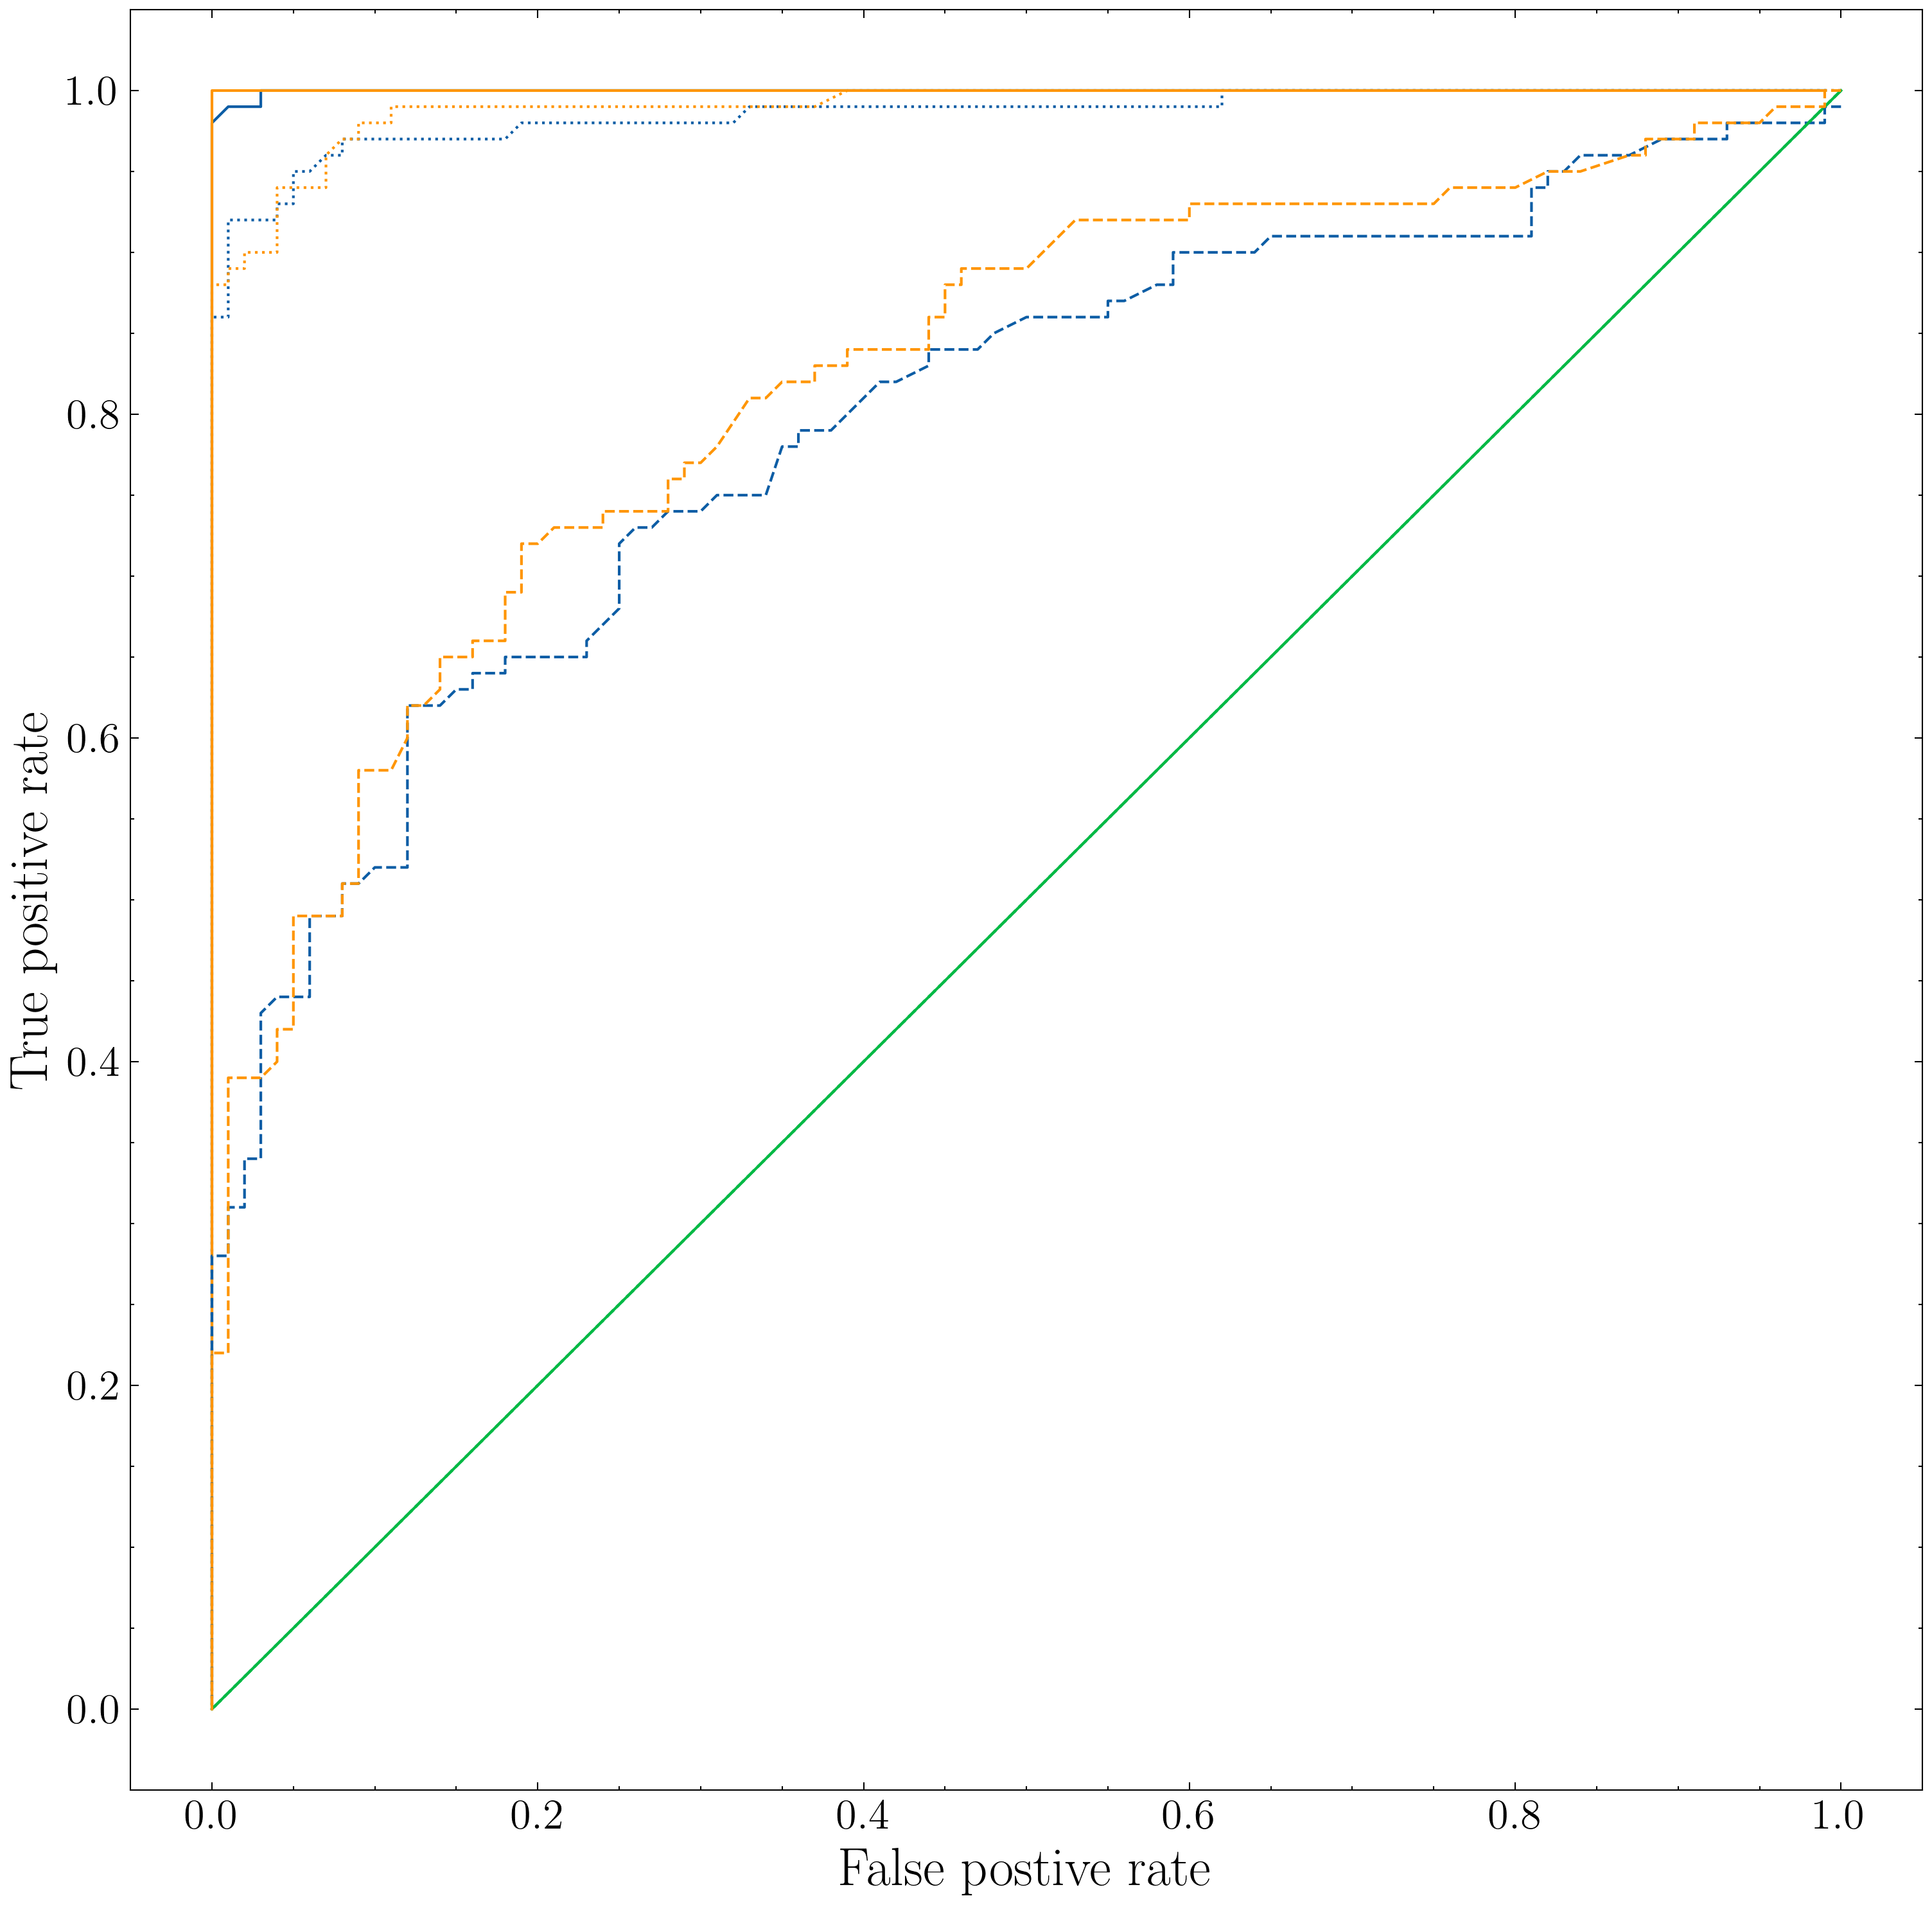
\includegraphics[width=\columnwidth]{images/roc_final_stacked.png}
%	\end{center}
%	\caption{ROC curve for 3 different systems $\{ \gamma = 0.001, \Delta f = 0.0\}$, $\{ \gamma = 0.01, \Delta f = 0.0\}$ , $\{ \gamma = 0.01, \Delta f = 0.5\}$ (dotted, dashed, solid respectively). The green lines denote the Viterbi search run without any ANC filtering, the blue lines with ANC filtering with 1 reference channel and the orange line with 2 reference channels. ANC filtering using 2 reference channels consistently outperforms that using a single reference channel.}
%	\label{fig:roc3}
%\end{figure}



%As discussed the ARLS filter has 2 parameters that can be freely chosen, the forgetting factor $\lambda$ and the model order (i.e. the number of taps in the FIR filter), $M$. For this work we have set $\lambda$ to a fixed value of $\lambda = 0.9999$. 




%
%
%

%\textcolor{red}{Changrong:} If we simply add more reference signals without normalizing the amplitude, it will definitely result in better performance (this is like we increase $|H(w)|$). But if we normalize the amplitude $a_r$ by $a_r/L$ with $L$ the number of references, we will not see obvious improvement.
%
%It might be the overfitting problem Rob mentioned previously, where with the number of taps chosen sufficiently large, it might already be enough to capture the dynamics of the interference signal without adding new interferences.
%
%But if we have multiple independent interference sources, with each reference correlated to each interference, then I suppose we should add more references.
%
%



\section{Conclusions}\DIFaddbegin \label{sec:conclusions}
\DIFaddend In this paper we demonstrate a new line subtraction method based on adaptive noise cancellation for use in continuous gravitational wave searches. We use an adaptive recursive least squares method in conjunction with an independent, known PEM reference signal to suppress the interference from a long-lived narrow spectral feature. We then search for the continuous wave signal using a HMM Viterbi algorithm. We test our method on synthetic data containing the 60 Hz spectral interference line due to the North American power grid. We show how the the ANC and Viterbi algorithm together are able to successfully track the spin-wandering continuous GW signal near the 60 Hz line. \DIFdelbegin \DIFdel{We test the method over multiple noise realisations and show \textcolor{red}{TK: to confirm}. The performance of the filter is generally improved with an increased number of reference signals and at an increased model order}\DIFdelend \DIFaddbegin \DIFadd{The method is shown to be robust to different mains power interference parameters, whilst larger values of $N_{\rm ref}$, $M$ and $\lambda$ generally increase the effectiveness of the ANC filter and the probability of detecting the GW signal}\DIFaddend .



%This is a conclusion 


%\appendix
%\subfile{anc-app}
%\label{app:failedMs}


\newpage 
\newpage 

\appendix


%\begin{figure}[h!]
%	\begin{center}
%		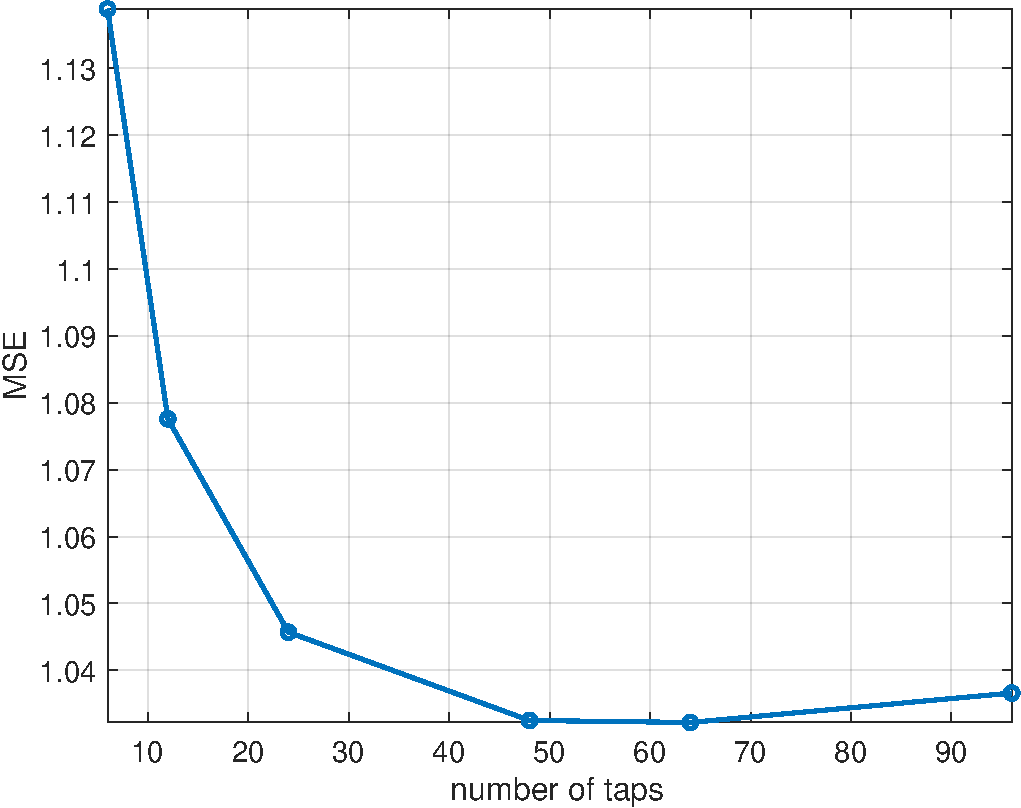
\includegraphics[width=0.49\textwidth]{result_images/mse_tap.pdf}
%	\end{center}
%	\caption{\label{mse vs tap}
%		Mean square error: MSE as a function of number of taps with $|H(w)|=3$ and $\rm{SNR}_{\rm in}=0.02$.}
%\end{figure}

















%
%\begin{figure*}
%	\begin{center}
%		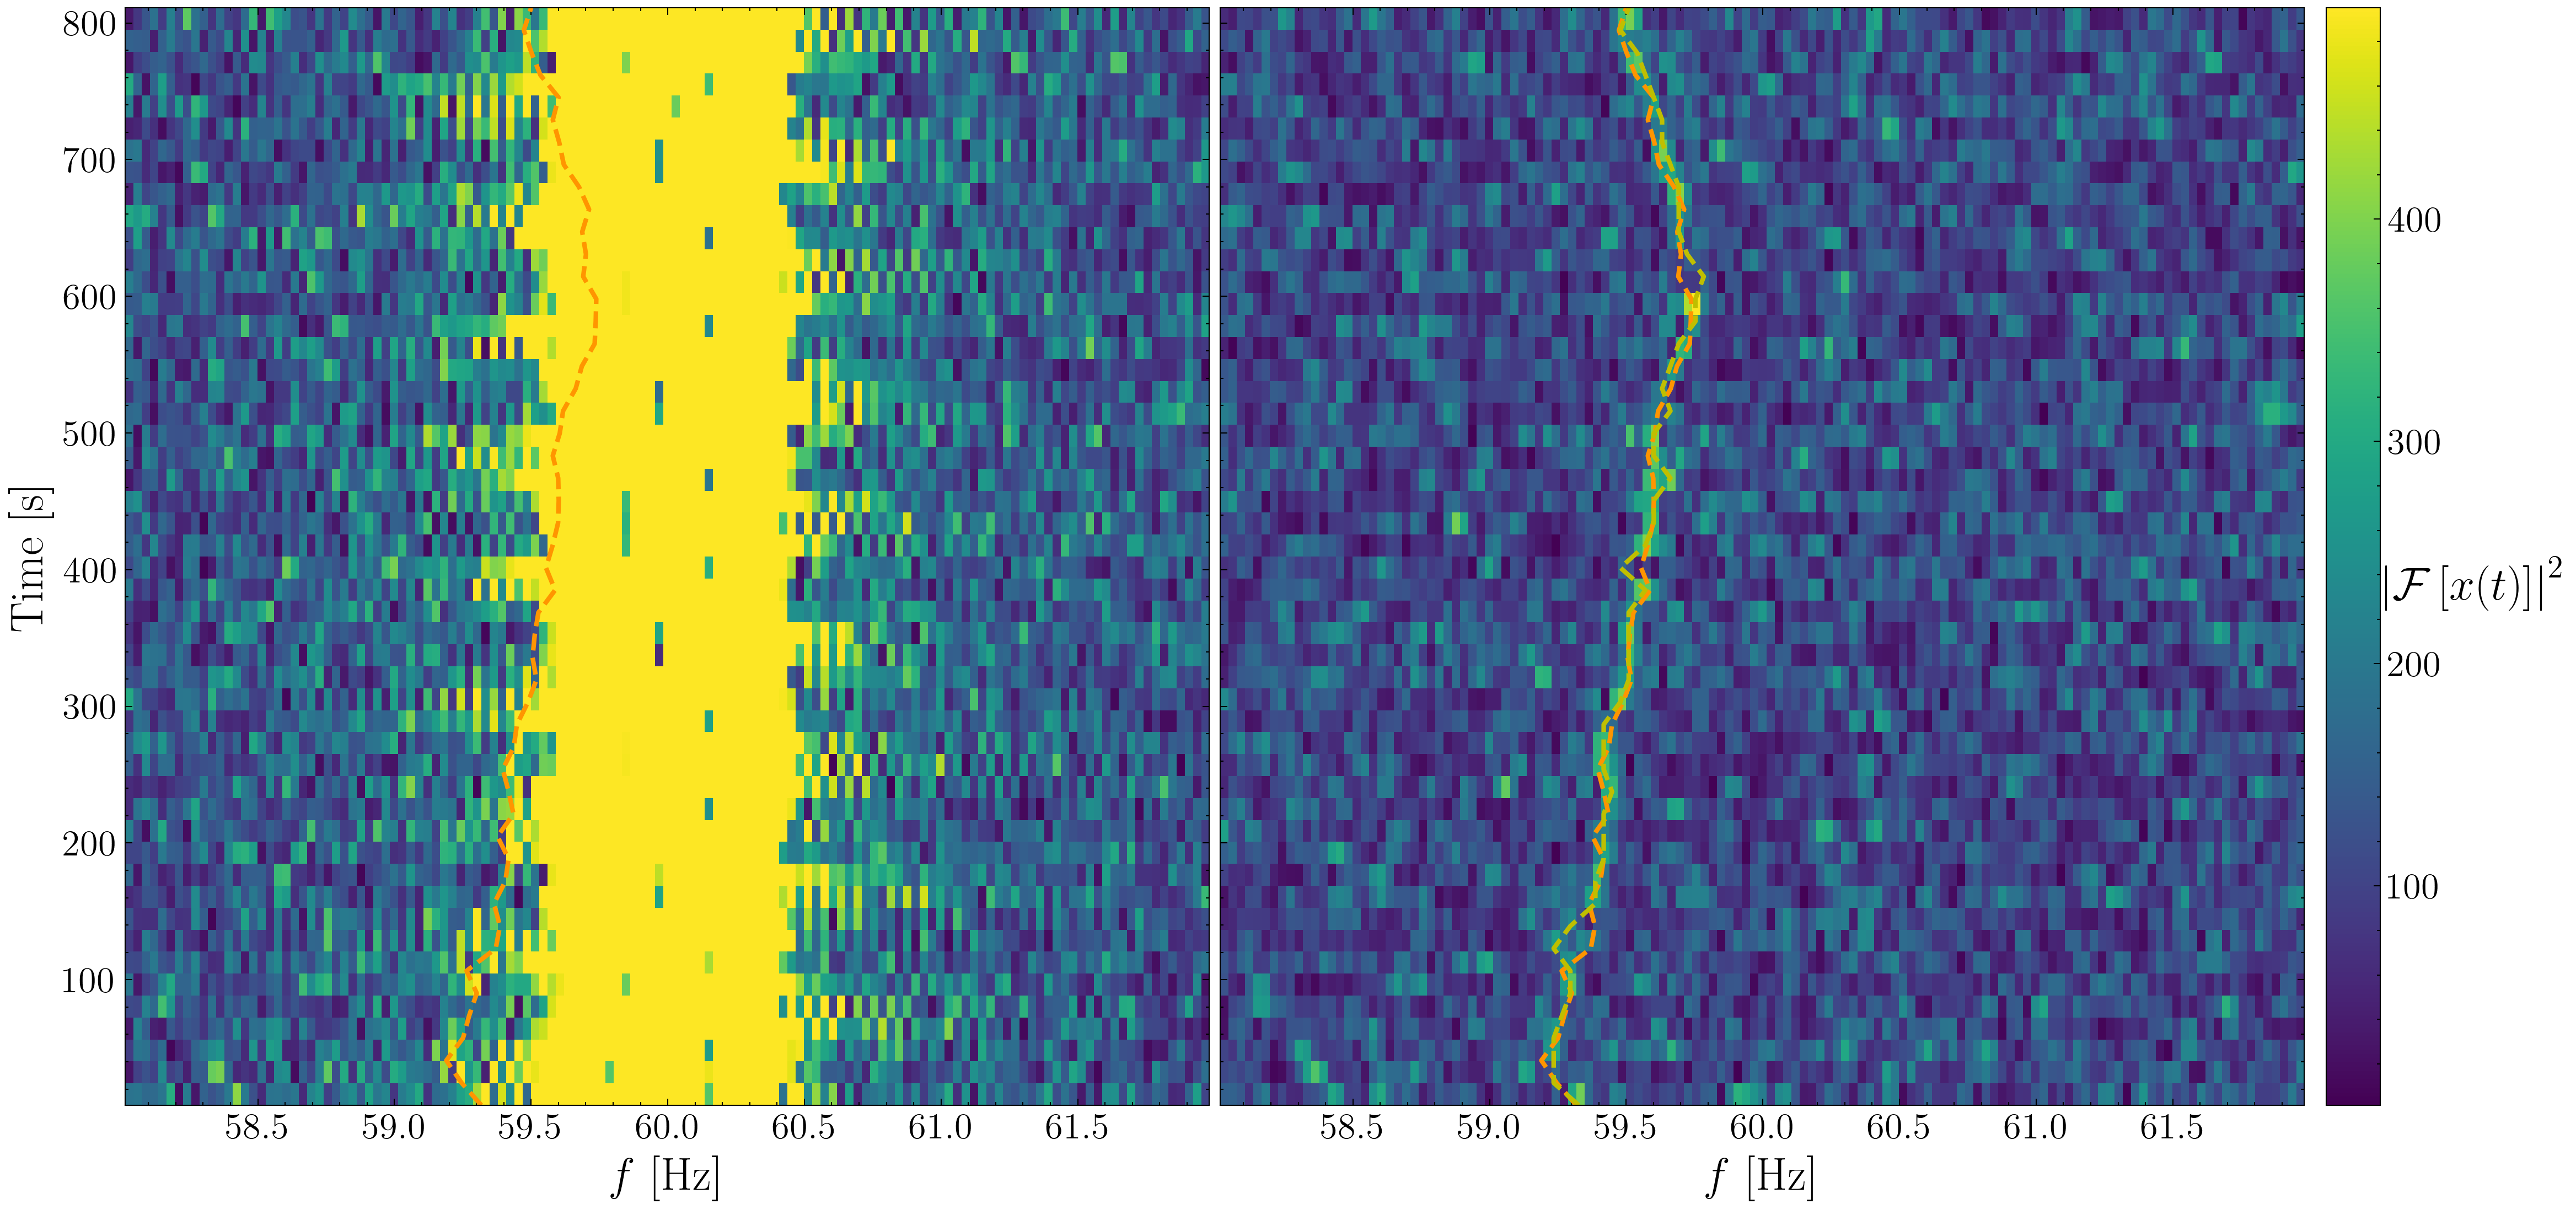
\includegraphics[width=\textwidth]{images/ANC_shared_y_example_1_high_contrast}
%	\end{center}
%	\caption{\label{frequency tracking before and after1high}
%		Tracking of the frequency evolution of a continuous GW with SNR$_{\rm in} = 0.025$, $H(\omega) =4$ and $\Delta f = 0.5$ using a HMM Viterbi algorithm both before (left hand panel) and after (right hand panel) the application of the ANC filter to remove the interference signal centred at 60Hz. The GW signal is indicated by diagonal dashed line. \textcolor{red}{TK: high contrast version also available. What are the settings?}}
%\end{figure*}
%
%
%
%\begin{figure*}
%	\begin{center}
%		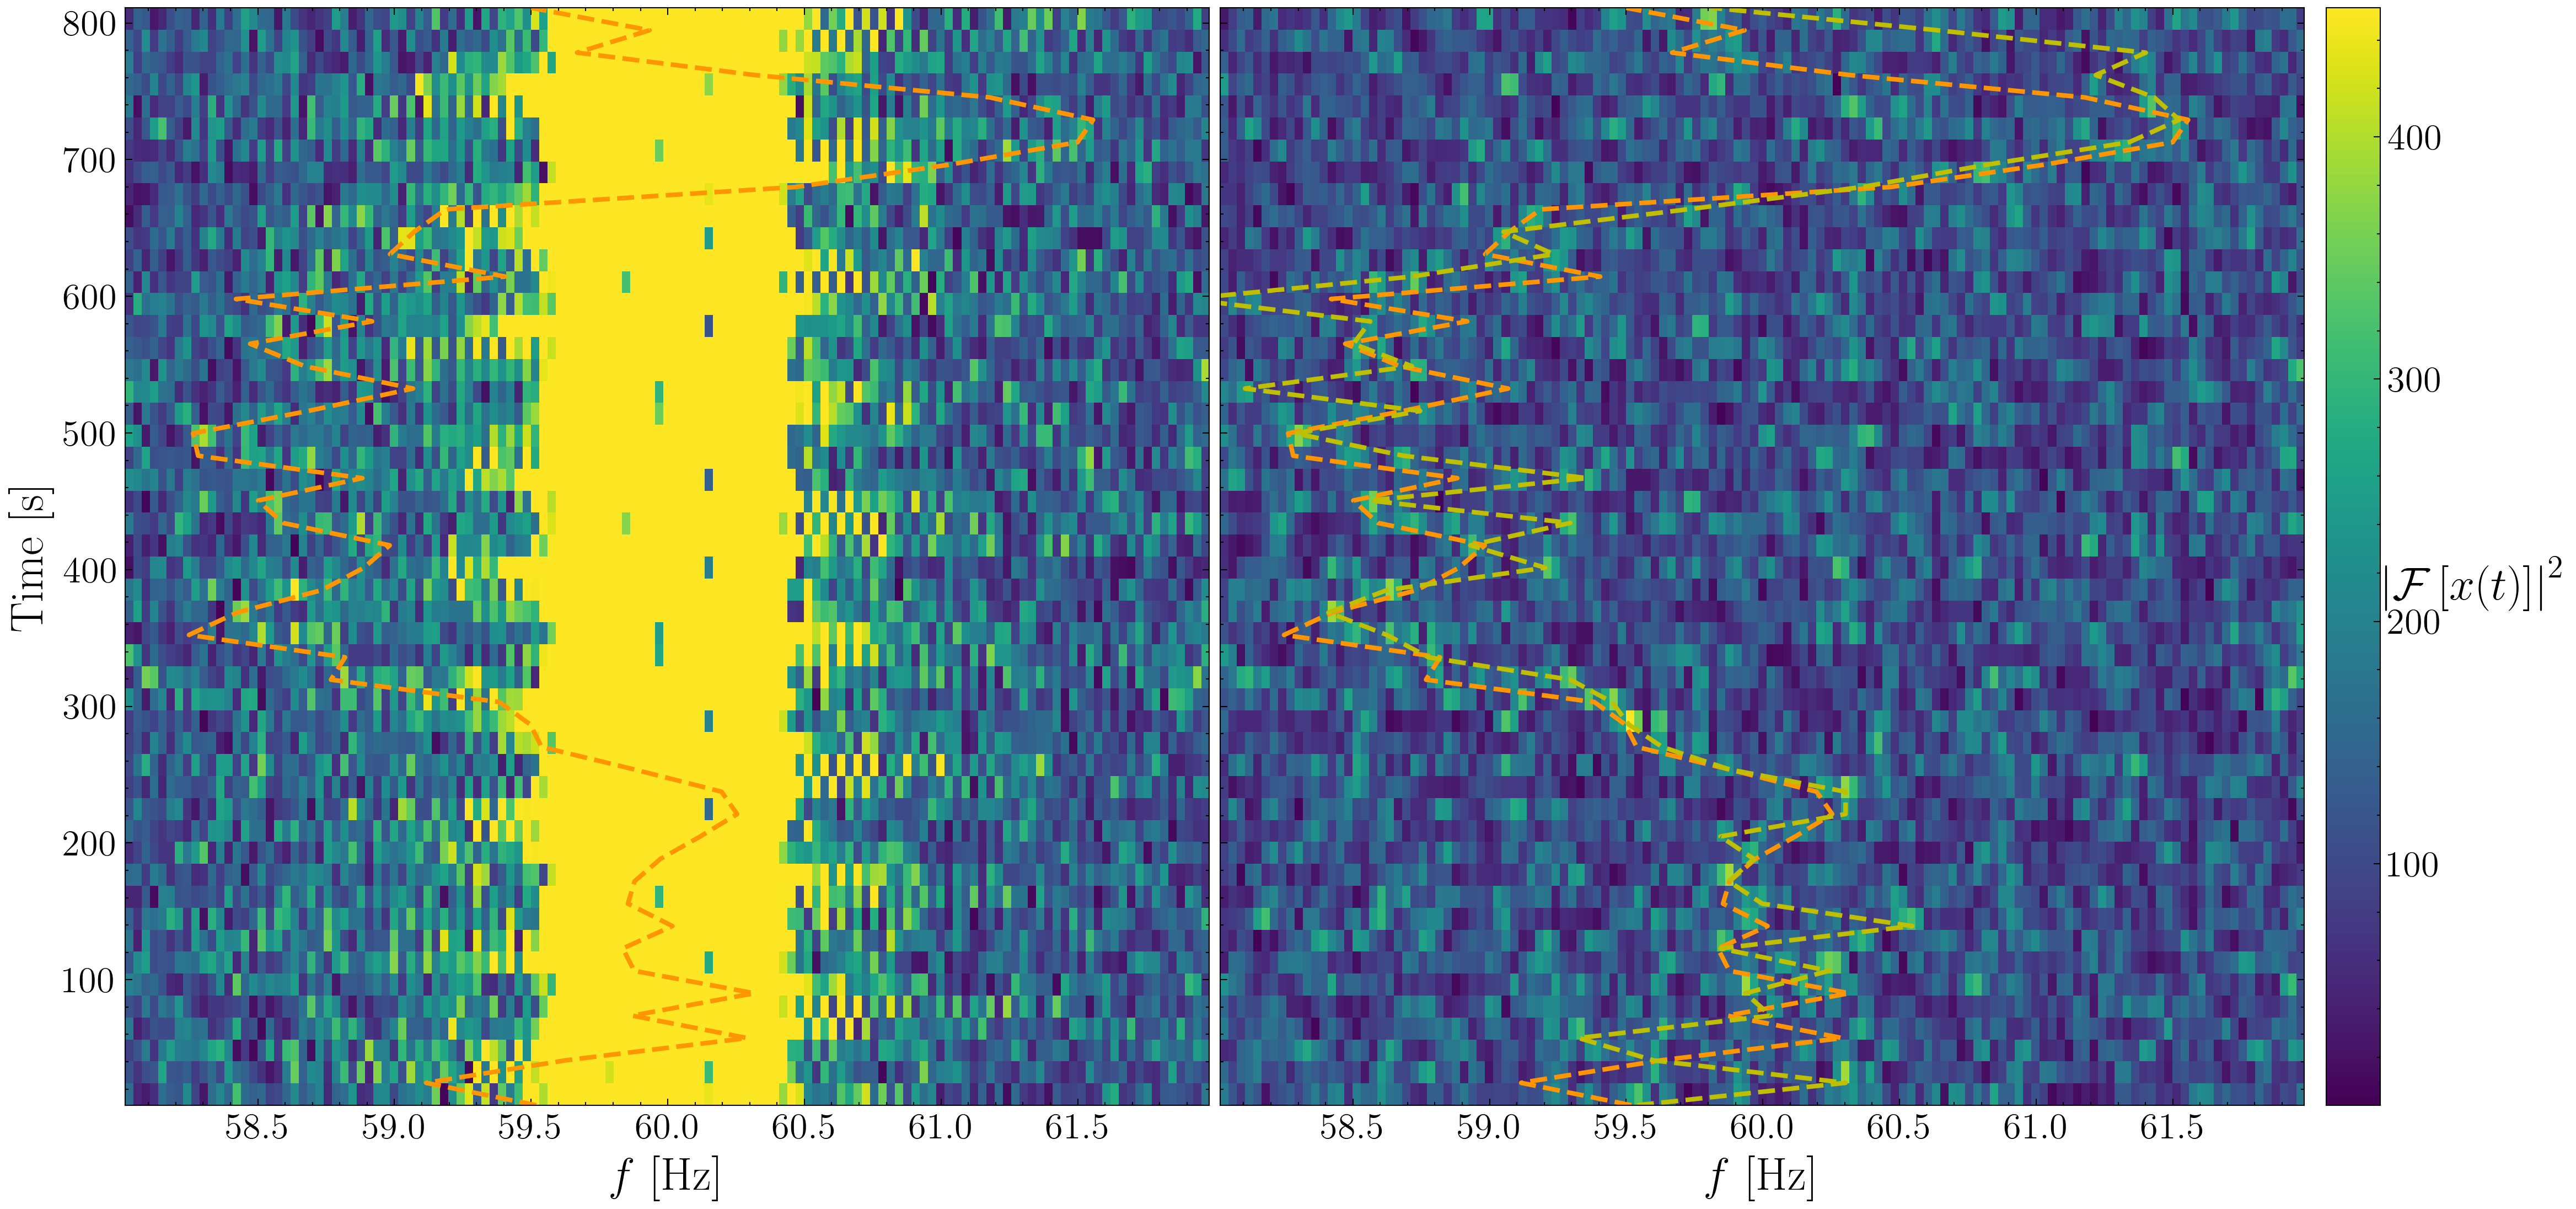
\includegraphics[width=\textwidth]{images/ANC_shared_y_example_2_high_contrast}
%	\end{center}
%	\caption{\label{frequency tracking before and after2high}
%		Tracking of the frequency evolution of a continuous GW with SNR$_{\rm in} = 0.025$, $H(\omega) =4$ and $\Delta f = 0.5$ using a HMM Viterbi algorithm both before (left hand panel) and after (right hand panel) the application of the ANC filter to remove the interference signal centred at 60Hz. The GW signal is indicated by diagonal dashed line. \textcolor{red}{TK: high contrast version also available. What are the settings?}}
%\end{figure*}
%
%
%




%
%
%
%
%\section{Old material}
%
%
%
%
%
%\begin{figure*}
%	\begin{center}
%		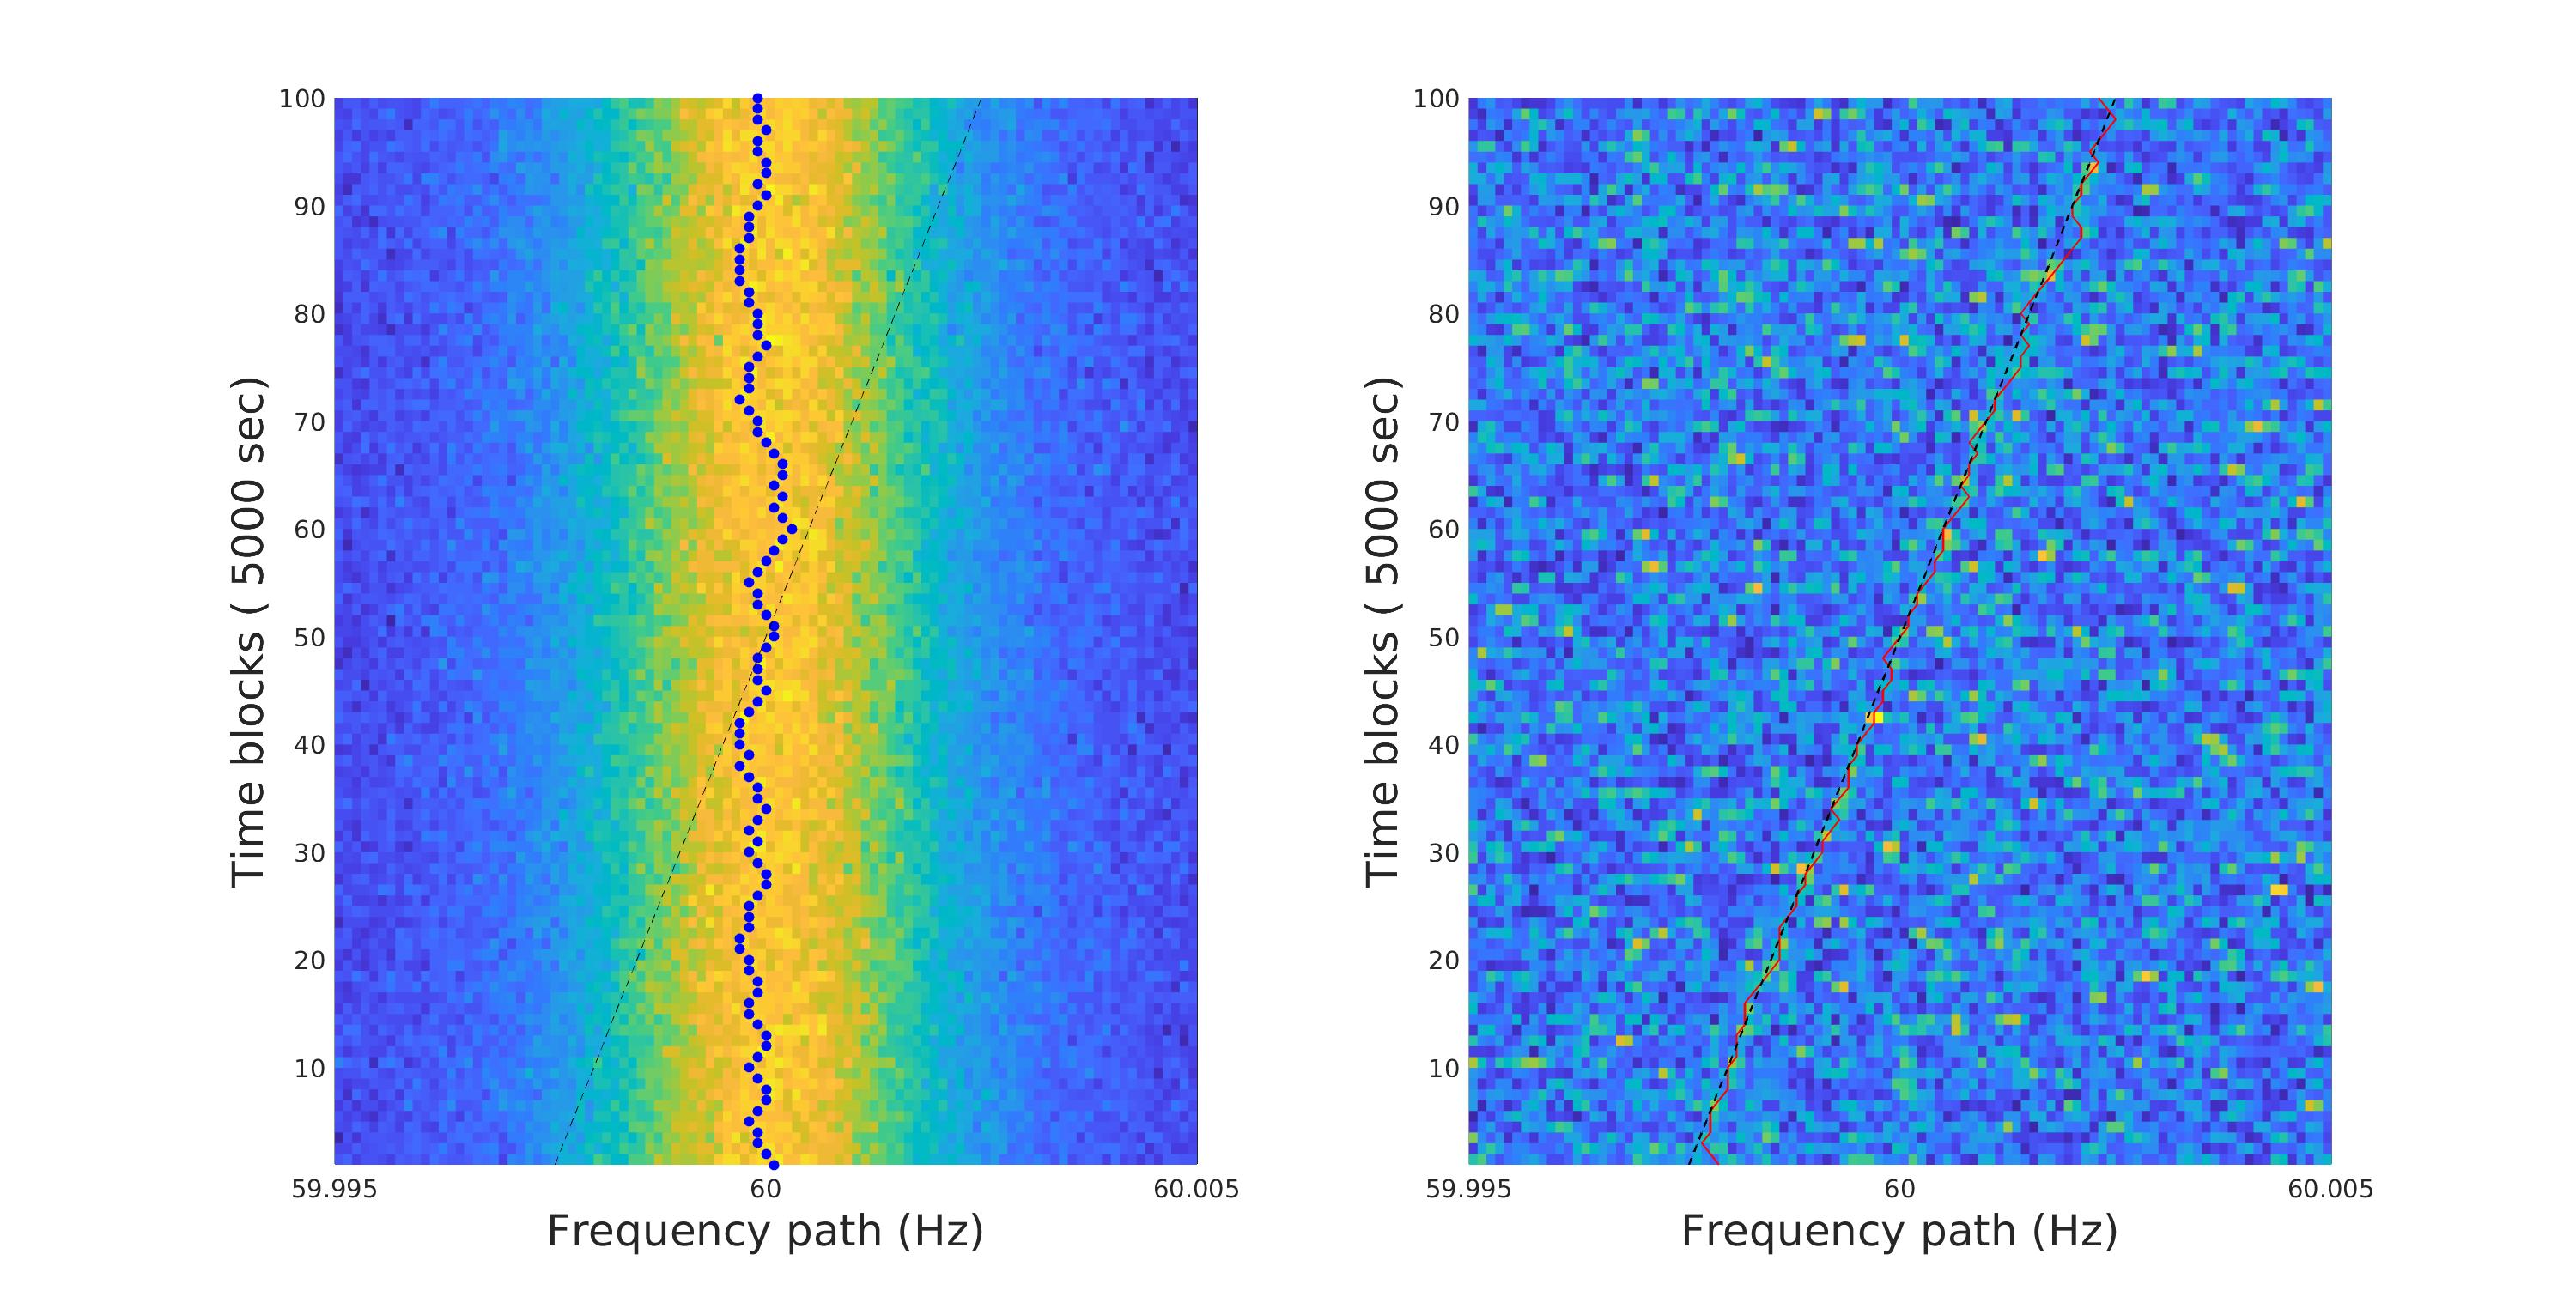
\includegraphics[width=\textwidth]{result_images/before_and_after.jpg}
%	\end{center}
%	\caption{\label{frequency tracking before and after}
%		Tracking of the frequency evolution of a continuous GW with SNR$_{\rm in} = 0.025$, $H(\omega) =4$ and $\Delta f = 0.5$ using a HMM Viterbi algorithm both before (left hand panel) and after (right hand panel) the application of the ANC filter to remove the interference signal centred at 60Hz. The GW signal is indicated by diagonal dashed line. \textcolor{red}{TK: What is the y axis? This should be two separate figures. Make red line clearer in RHS}}
%\end{figure*}
%
%
%
%
%\begin{figure}[h!]
%	\begin{center}
%		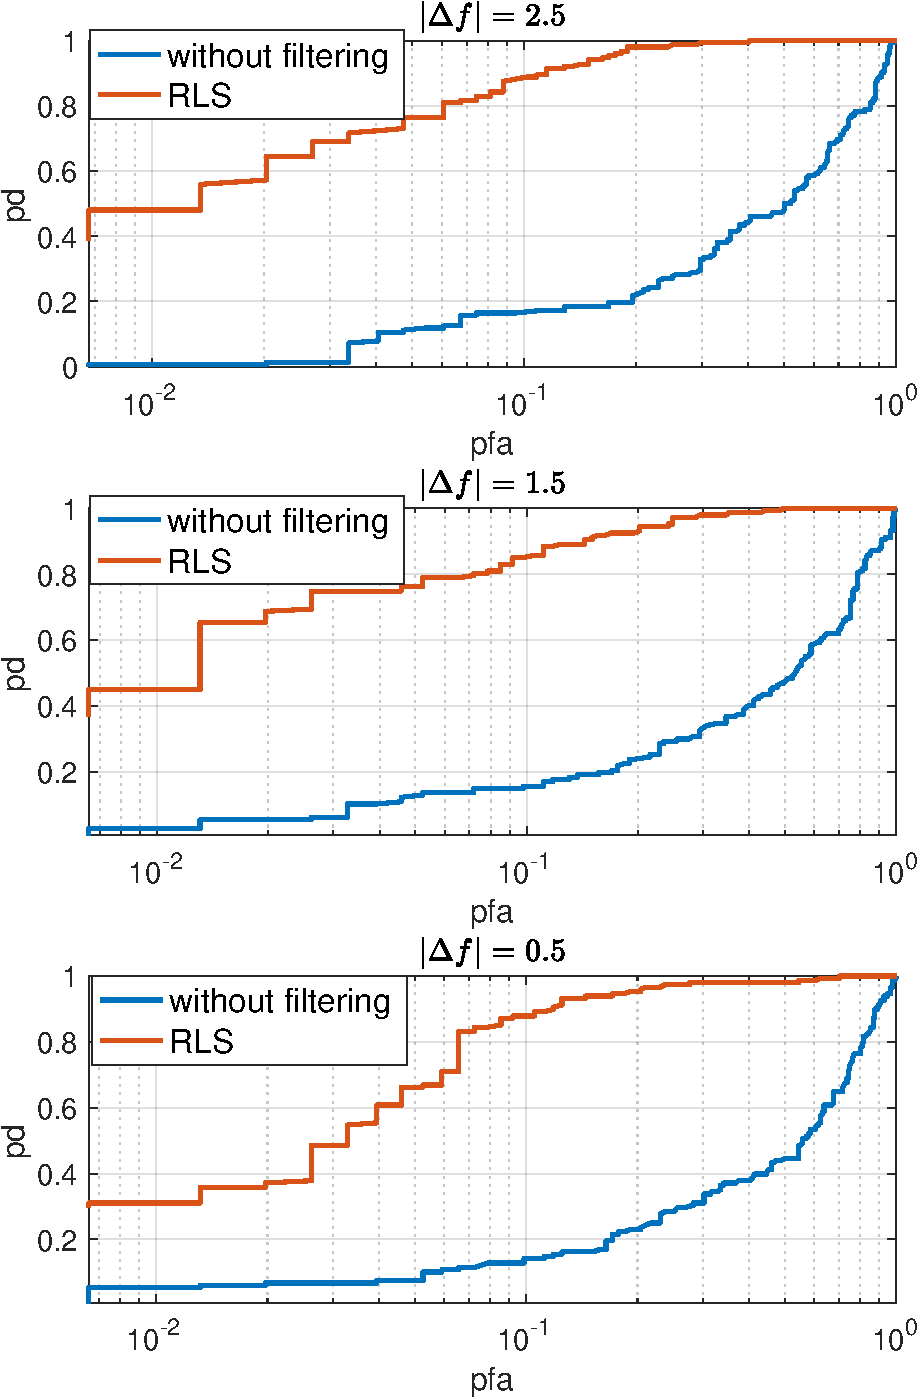
\includegraphics[width=0.49\textwidth]{result_images/frequency_difference_crop.pdf}
%	\end{center}
%	\caption{\label{fig:frequency difference}
%		ROCs under different $\Delta f$ with $|H(w)|=3$ and $\rm{SNR}_{\rm in}=0.025$}
%\end{figure}
%\begin{figure}[h!]
%	\begin{center}
%		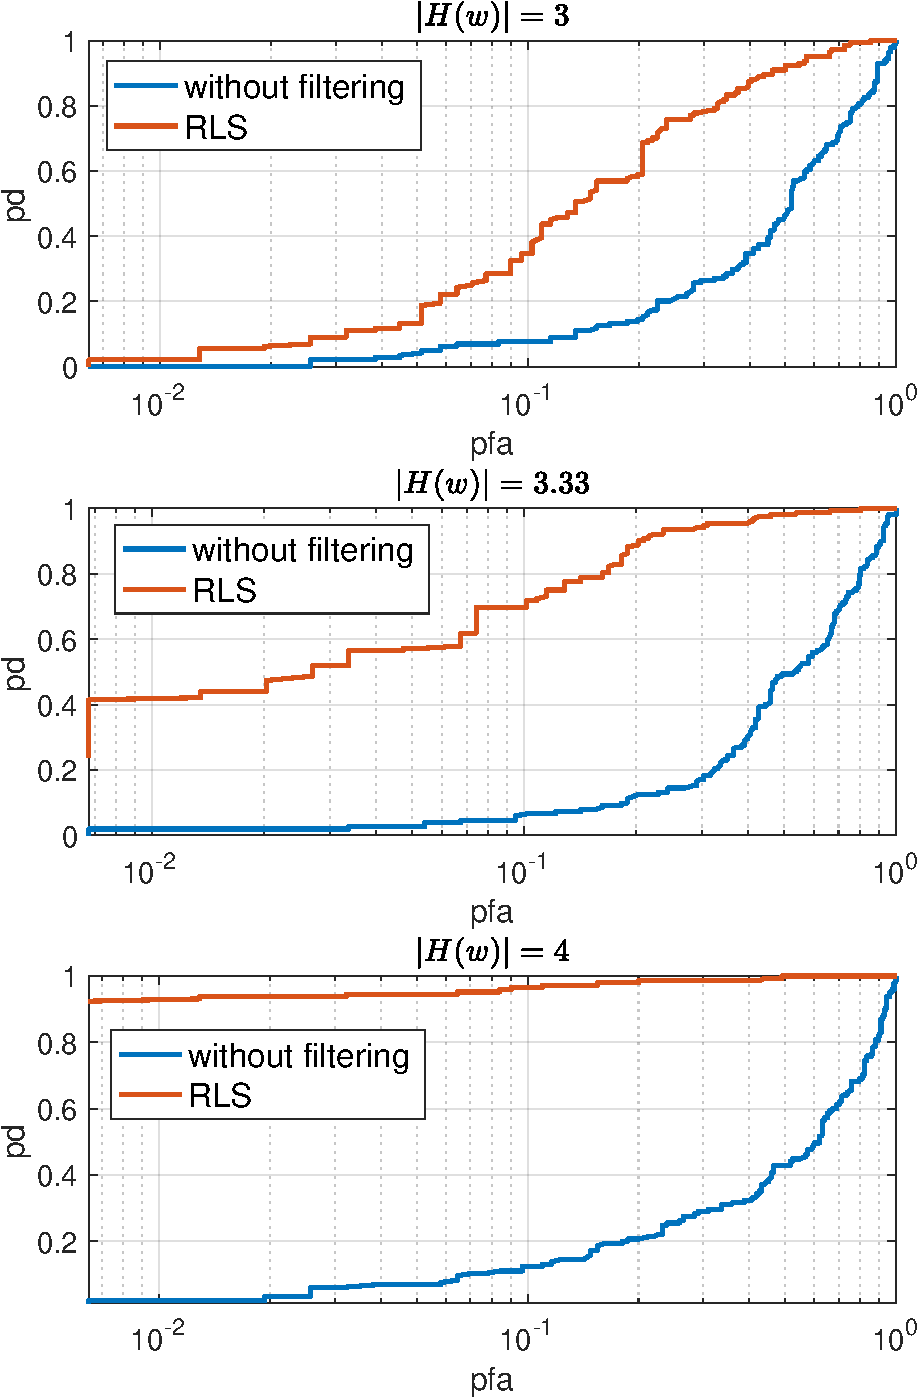
\includegraphics[width=0.49\textwidth]{result_images/homega_crop.pdf}
%	\end{center}
%	\caption{\label{fig:H(w)}
%		ROCs under different $|H(w)|$ with $\Delta f=0.5$ and $\rm{SNR}_{\rm in}=0.02$ \textcolor{red}{TK:change ordering of subplots so both delta f and H increase}}
%\end{figure}
%
%
%
%\begin{figure}
%	\begin{center}
%		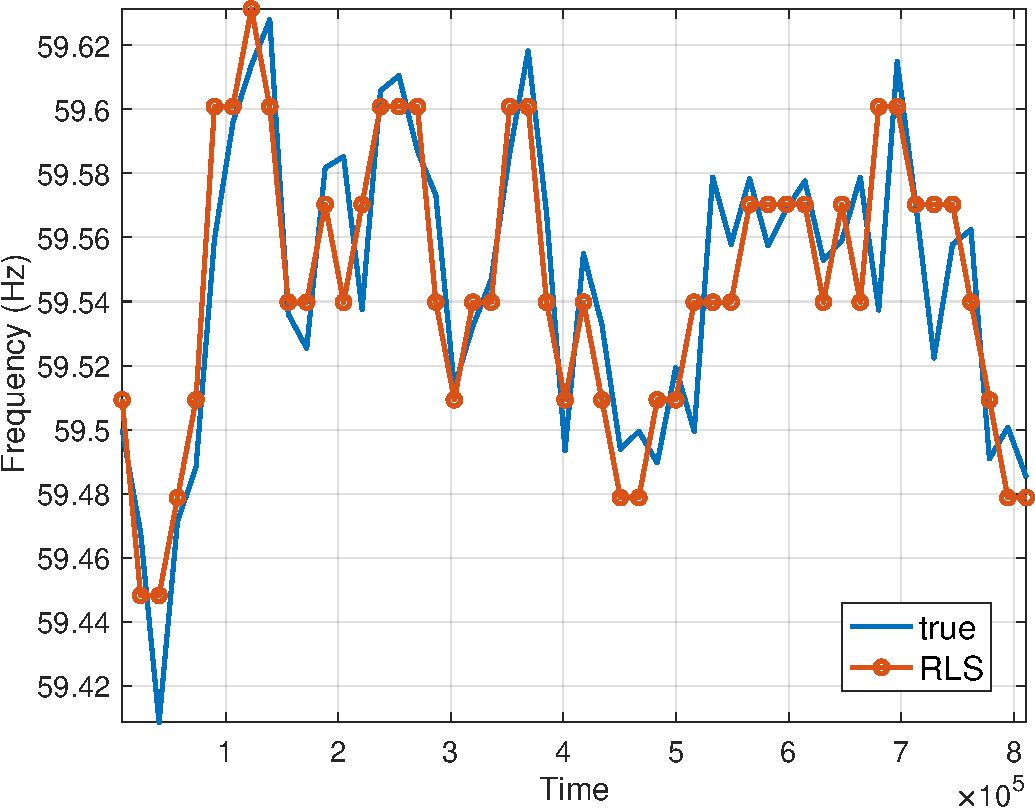
\includegraphics[width=0.49\textwidth]{result_images/frequency_tracking.pdf}
%	\end{center}
%	\caption{\label{frequency tracking}
%		Frequency tracking after RLS: $\rm{SNR}_{\rm in}=0.025$, $\Delta f = 0.5$, $|H(w)|=4$. \textcolor{red}{TK: Update this figure. Remove legend. Is this interference frequency or gw frequency?}}
%\end{figure}
%
%\begin{figure}
%	\begin{center}
%		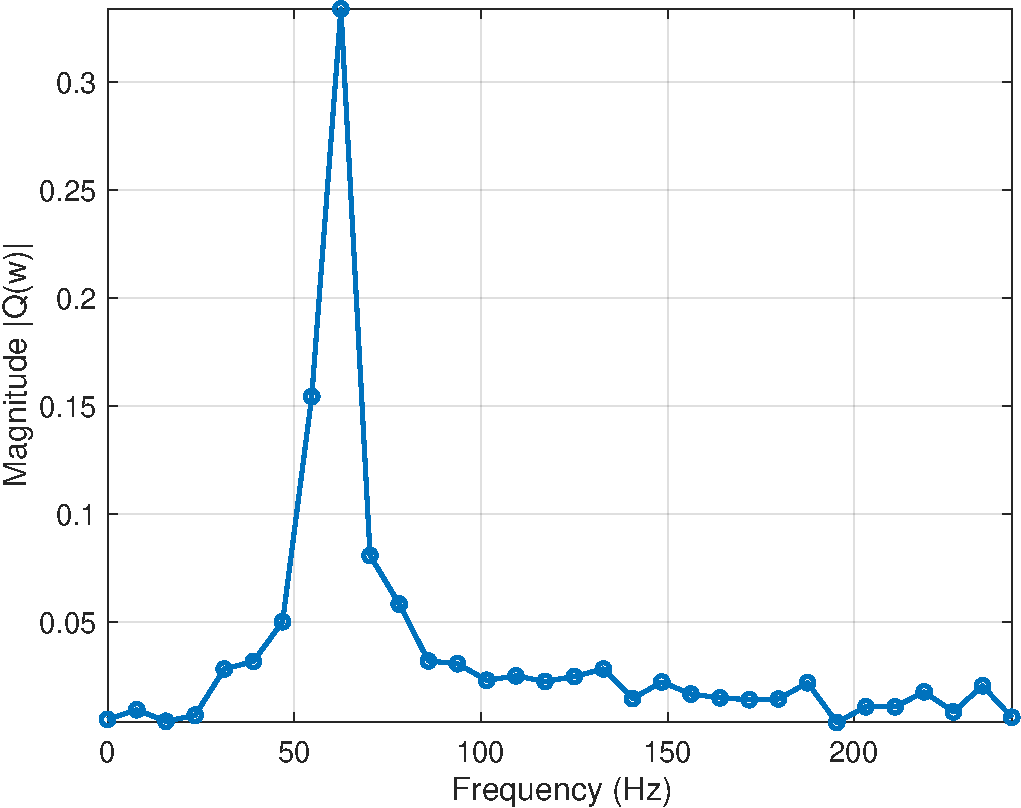
\includegraphics[width=0.49\textwidth]{result_images/taps2_frequency.pdf}
%	\end{center}
%	\caption{\label{taps_freq}
%		Frequency spectrum of the adaptive filter after converging. \textcolor{red}{TK: Update caption TBD}}
%\end{figure}
%
%
%\begin{figure}
%	\begin{center}
%		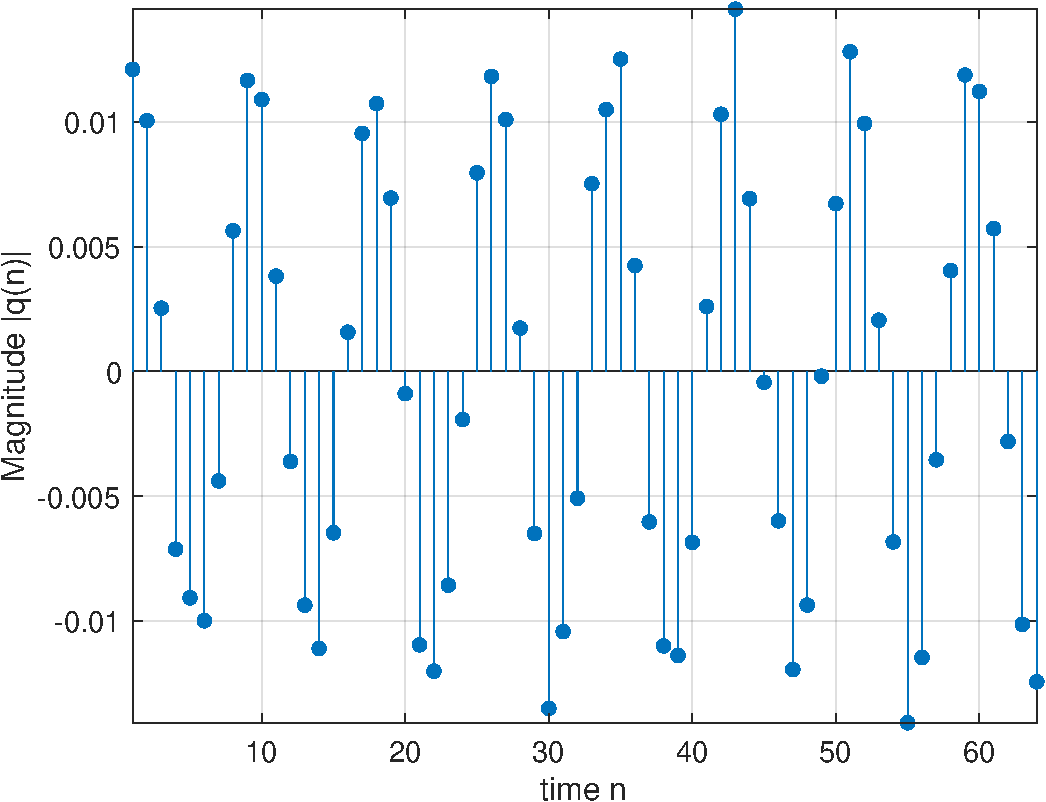
\includegraphics[width=0.49\textwidth]{result_images/taps2_time.pdf}
%	\end{center}
%	\caption{\label{taps}
%		Impulse response of the adaptive filter after converging. \textcolor{red}{TK: Clean up figure e.g. axis labels What is the x axis?}}
%\end{figure}




%\bibliographystyle{myunsrt}
\bibliographystyle{apsrev4-1} % Tell bibtex which bibliography style to use

\bibliography{bibLinesPaper}
%%%%%%%%%%%%%%%%%%%%%%%%%%%%%%%%%%%%%%%%%%%%%%%%%%


\begin{acknowledgements}
%GWOSC
This research has made use of data, software and/or web tools obtained from the Gravitational Wave Open Science Center (https://www.gw-openscience.org), a service of LIGO Laboratory, the LIGO Scientific Collaboration and the Virgo Collaboration. LIGO is funded by the U.S. National Science Foundation. Virgo is funded by the French Centre National de Recherche Scientifique (CNRS), the Italian Istituto Nazionale della Fisica Nucleare (INFN) and the Dutch Nikhef, with contributions by Polish and Hungarian institutes\DIFaddbegin \DIFadd{. This research was supported by
the Australian Research Council Centre of Excellence for Gravitational Wave Discovery (OzGrav), grant number CE170100004}\DIFaddend .
\end{acknowledgements}


\end{document}

